\documentclass[12pt]{book} 

% TODO: create an inline \code command for monospace font

% The document preamble 

\usepackage[superscript,biblabel]{cite}

\usepackage{makeidx}



\usepackage{amssymb} % math notation (R)

\usepackage{url}
\usepackage[dvipsnames]{xcolor} % needs to loaded before \usepackage{markdown}
% had to add --shell-escape to pdflex command
\usepackage{markdown}
%\usepackage[hashEnumerators,smartEllipses]{markdown}

\usepackage{times} % Use PS times fonts 

\usepackage{listings} % code examples
 % textcolor

\usepackage{multirow}
\usepackage{rotating}
\usepackage{titlesec} % for using paragraphs as a "subsubsubsection"

% for encoded images
%\usepackage{filecontents}
%\newcommand{\generateimage}[2]{%
%\immediate\write18{convert.cmd #1 > #2}}
\usepackage{graphicx}	% Use pdf, png, jpg, or eps§ with pdflatex; use eps in DVI mode

\usepackage{enumitem}

\makeindex 

% https://tex.stackexchange.com/questions/45711/defining-lstset-parameters-for-multiple-languages
% Copied from the listings documentation
\lstdefinestyle{numbers} {numbers=left, stepnumber=1, numberstyle=\tiny, numbersep=10pt}
\lstdefinestyle{pyinput}{backgroundcolor=\color{gray!8},frame=shadowbox,showspaces=false, basicstyle=\scriptsize }
\lstdefinestyle{pyoutput}{backgroundcolor=\color{green!8},frame=shadowbox,showspaces=false, basicstyle=\scriptsize }
\lstdefinestyle{terminal}{backgroundcolor=\color{gray!8},frame=shadowbox,showspaces=false, basicstyle=\scriptsize }

% TODO: need common code style
\def\code#1{\texttt{#1}}

% used to determine level of rough-drafted-ness, where r= most rough, rrr= presumably less rough (3 passes)
\def\r#1{\textcolor{SeaGreen}{#1}}
%SpringGreen
\def\rr#1{\textcolor{ProcessBlue}{#1}}
\def\rrr#1{\textcolor{NavyBlue}{#1}}
\def\TD#1{\textcolor{green}{#1}}

%% indexing w/it and w/o it
\def\IDI#1{{\textit{#1}}\index{#1}}
\def\ID#1{{#1}\index{#1}}

\def\ALR{\textcolor{red}{ADD LOCAL REF}}



% breaklines=true is used to wrap lines
\lstdefinestyle{pyOutStyle} {language=Bash,style=numbers,style=pyoutput,frame=none}
\lstdefinestyle{terminalBash} {language=Bash,style=numbers,style=terminal,frame=lines, breaklines=true}

% captions for equations
\usepackage{caption}
\DeclareCaptionType{equ}[][]

% for python snippets
\usepackage{pythonhighlight}


% Details of the titlepage 
\title{Teaching a Computer to Fish: Machine+Deep Learning with YeahML} 
\author{Jack Burdick} 
\date{Last Update: \today} % Use the system date

% for using paragraphs as a "subsubsubsection"
\setcounter{secnumdepth}{4}
\setcounter{tocdepth}{4}
\titleformat{\paragraph}
{\normalfont\normalsize\bfseries}{\theparagraph}{1em}{}
\titlespacing*{\paragraph}
{0pt}{3.25ex plus 1ex minus .2ex}{1.5ex plus .2ex}

\begin{document} 
	
\frontmatter

\maketitle 

\tableofcontents


\mainmatter

\part{Background}

\chapter{Introduction}

But if you teach your computer to fish..

% intro

% motivation
There are many great resources that exist.

I wanted to create the guide I wish I found when I started learning tensorflow.


%
\textcolor{blue}{ML -- study of how programs learn from data}

\textcolor{blue}{Arthur Samuel -- ``ML is the study that gives computers the ability to learn without being explicitly programed.''}

\textcolor{blue}{Tom Mitchel -- ``A program can be said to learn from experience `E' with respect to some class of tasks `T' and performance measure `P', if its performance at tasks in `T', as measured by `P', improves with experience `E'.''}

\chapter{Resources and Communities}

\textcolor{blue}{There are many great resources and communities that I'd like to highlight}


\section{Online Communities}

\begin{itemize}[noitemsep,topsep=0pt]
	
	\item Reddit
	
	\item Stack Overflow
	
	\item Slack
\end{itemize}


\section{Blogs}

\begin{itemize}[noitemsep,topsep=0pt]
	
	\item \textcolor{blue}{XXXXXXXXXXXXXXX}
	
\end{itemize}



\section{Online Courses}

\begin{itemize}[noitemsep,topsep=0pt]
	
	\item Udacity
	\item Coursera
	\item Udemy
	
	\item \textcolor{blue}{XXXXXXXXXXXXXXX}
	
\end{itemize}


\section{Text Books}

\begin{itemize}[noitemsep,topsep=0pt]
	\item \textcolor{blue}{XXXXXXXXXXXXXXX}
	
\end{itemize}

\chapter{Prerequisites}

\textcolor{blue}{The following sections are a non-exhaustive, brief, refresher on some of the important underlying concepts and methodologies used by later concepts. Resources to further explore and learn these concepts are shared.}

\textcolor{blue}{But first, let's start by answering the million dollar question: what the heck is a tensor?  A {tensors}\index{tensor} are a generalization of matrices and can have an arbitrary number of dimensions (axis). The number of axes tensors of a tensor is also called the {rank}\index{rank}.}


\section{Math Notation}

\textcolor{blue}{Depending on the resource, the level of formal math education required to understand a passage may vary greatly. In order to demystify some of the resources that do not expand on the proofs and notations, below are some of the symbols and XXXXX used in math notation and their interpretation in simple text/natural language form.}

\textcolor{green}{TODO: Show symbols and examples in both equation and simple text/natural language form.}

\textcolor{blue}{$\mathbb{R}$}

\section{Calculus}

\textcolor{yellow}{Don't worry we won't be proving any theorems and I won't be assigning 45 questions due tomorrow. But, there is some basic terminology that should be revisited.}

\textcolor{blue}{{Critical points}\index{Critical points} or {stationary points}\index{stationary points} are points where the derivative is equal to zero and therefore doesn't provide any useful information about the gradient/slope (which direction and how far to move)}

\begin{figure}
	\centering
	\includegraphics[width=0.5\textwidth]{example-image-a}\hfil
	\caption{Graph of an example function and its derivative, \textcolor{green}{TODO}}
	\label{fig:calc_fn_deriv}
\end{figure}
\textcolor{green}{TODO: graph of function and it's derivative overlaid.}

\textcolor{blue}{There exist three main types of critical points:}

\begin{itemize}
	\item \textcolor{blue}{local minimum} -- 
	\item \textcolor{blue}{local maximum} -- 
	\item \textcolor{blue}{saddle point} -- 
\end{itemize}

\begin{figure}[htp]
	\centering
	\includegraphics[width=0.3\textwidth]{example-image-a}\hfil
	\includegraphics[width=0.3\textwidth]{example-image-b}\hfil
	\includegraphics[width=0.3\textwidth]{example-image-c}
\caption{Types of critical points -- points with zero slope. From left to right, \textcolor{green}{TODO}}
\label{fig:calc_critical_points}
\end{figure}


\textcolor{blue}{Functions may have many local minimal and plateaus. The point at which the absoluet lowest value is considered the {global minimum}\index{global minimum}. Similarly a value located at the largest absolute value of the function is considered the {global maximum}\index{global maximum}. }

\begin{figure}
	\centering
	\includegraphics[width=0.5\textwidth]{example-image-b}\hfil
	\caption{Graph of an example function with many (labeled) local minima and plateaus. the global minima should also be labeled. \textcolor{green}{TODO}}
	\label{fig:calc_fn_deriv}
\end{figure}

\subsection{Chain Rule}

\textcolor{blue}{(not the chain rule of probability)}



\section{Boolean Logic}

\textcolor{green}{TODO: background/overview on boolean logic and importance}

\textcolor{green}{TODO: Examples}


\section{Linear Algebra}

\subsection{Overview}

\textcolor{green}{TODO: background/overview on linear algebra and importance}

\textcolor{green}{TODO: Examples}

\subsubsection{Scalars (0D tensors)}

\textcolor{green}{TODO: diagram}

\textcolor{blue}{scalar -- single value (not a vector or matrix)}

\textcolor{green}{example: a single value}



\subsubsection{Vectors (1D tensors)}

\textcolor{green}{TODO: diagram}

\textcolor{blue}{vectors -- denoted by lowercase names}

\textcolor{blue}{vector: an $n x 1$ matrix. A $12 x 1$ vector may be considered a 12 dimension vector.}

\textcolor{blue}{1-indexed or 0-indexed. In this document, we will only use 0-indexed terms}

\textcolor{green}{example: a ``list'' of features}


\subsubsection{Matrices (2D tensors)}

\textcolor{green}{TODO: diagram}

\textcolor{blue}{Matrix -- written as (rows x columns)}

\textcolor{blue}{$M_{i,j}$ means matrix entry at ($i$,$j$), or $i$th row, $j$th column}


\textcolor{blue}{Matrices -- denoted by uppercase names}

\textcolor{green}{example: a grayscale (single color channel image)}



\subsection{Matrix Arithmetic}

\textcolor{blue}{{element-wise}\index{element-wise} operations: operations that are applied independently to each entry. These types of operations lend themselves nicely to parallelization/vectorization}

\textcolor{blue}{dot product --- \textcolor{green}{TODO: visualization of dot product inputs and output}}

\subsubsection{Matrices}

\paragraph{Addition, Subtraction}

\paragraph{Multiplication, Division}

\subsubsection{Scalar}

\paragraph{Addition, Subtraction}

\paragraph{Multiplication, Division}



\section{Graph Theory}

\textcolor{green}{TODO: Examples}

\textcolor{blue}{computational graph}

\textcolor{blue}{operation}




\part{ML}

% the organization and sec structure/naming needs work here.
\chapter{Basics}

\section{Overview}

%%%%%%%%%%%%%%%%%%%%%%%% obligatory "No Free Lunch"
I'm not sure it's possible to discuss machine learning without at least mentioning the ``No Free Lunch'' theorem, which states ``No single classifier works best across all possible scenarios''

%%%%%%%%%%%%%%%%%%%%%%%% Types of data
\textcolor{blue}{categorical or numerical. Numerical can be discrete or continuous}

%%%%%%%%%%%%%%%%%%%%%%%% Measurement Levels
\textcolor{blue}{qualitative or quantitative.} 

\textcolor{blue}{Qualitative can be nominal (aren't numbers and can't be put in any order -- e.g. the seasons: spring, summer, fall, winter) or ordinal (groups and categories that follow a strict order -- e.g. difficult levels: hard, medium, or easy)}

\textcolor{blue}{Quantitative are represented by numbers but can be interval (0 is meaningless -- e.g. temperature in C or F, where true zero is not 0) or ratio (has a true 0 -- e.g. temperature in K, weight or length)}

\section{Workflow Overview}

% TODO: this will need to be checked+rechecked+redone
\textcolor{blue}{1. explore, 2. create datasets, 3. benchmark}


%%%%%%%%%%%%%%%%%%%%%%%% Bias
\section{Bias}
\label{sec:data_bias_overview}

\subsection{Types of Bias}

\subsubsection{Interaction Bias}

\subsubsection{Latent Bias}

\subsubsection{Selection Bias}

\subsubsection{Recency Bias}

\subsection{Evaluation}

\textcolor{blue}{Performance evaluation on subsets of your data}

\textcolor{blue}{Evaluating false positives and false negatives for these subsets in the context of the problem/application.}

\textcolor{blue}{Equality of Opportunity -- gives individuals an equal chance}


%%%%%%%%%%%%%%%%%%%%%%%% Acquiring Data
\section{Data Acquisition}


\subsection{Resources}

\subsection{Generating Fake Data}

\textcolor{green}{TODO: generating fake data with SKL}

\textcolor{blue}{make\_blobs}

% {{{datagen_blobs_2dcode}}}
\begin{lstlisting}[style=pyInStyle]
X, y = datagen.make_blobs(centers=4, n_samples=100, n_features=2,cluster_std=1.0,
                          center_box=(-10, 10),
                          random_state=42, shuffle=True)
\end{lstlisting}

% {{{datagen_blobs_2dimg}}}
\begin{figure}
\centering
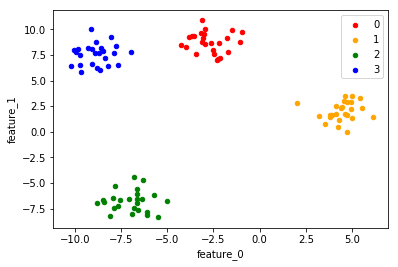
\includegraphics[width=0.65\textwidth]{./sync_imgs/datagen/blobs/2dimg.png}
\label{fig:datagen_blobs_2dimg}
\end{figure}

\textcolor{blue}{Data can also be generated in three (multiple) dimensions}

% {{{datagen_blobs_3dcode}}}
\begin{lstlisting}[style=pyInStyle]
X, y = datagen.make_blobs(centers=4, n_samples=100, n_features=3, random_state=42)
\end{lstlisting}

% {{{datagen_blobs_3dimg}}}
\begin{figure}
\centering
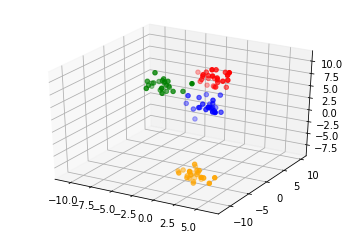
\includegraphics[width=0.65\textwidth]{./sync_imgs/datagen/blobs/3dimg.png}
\label{fig:datagen_blobs_3dimg}
\end{figure}

%\textcolor{blue}{More dataset types can be generated, the documentation can be found at (http://scikit-learn.org/stable/modules/classes.html#module-sklearn.datasets)}


\textcolor{blue}{see \textcolor{red}{local ref?} for more examples on how to generate data}


%%%%%%%%%%%%%%%%%%%%%%%% Data Pre-processing
\section{Data Preparation}

\textcolor{blue}{TODO: direct and indirect importance of datapreparation. indirect: feature engineering allows for more elegant and efficient solutions (e.g. calculating the time with a CNN of a clock face vs engineered features for the angles of the large and small hand.) }

\subsection{Data Pre-processing}

\textcolor{blue}{Data is rarely obtained in a form that is necessary for optimal performance of a learning algorithm. Data can be missing, can contain a mix of categorical and quantitative, can contain values on vastly different scales, etc.}

\textcolor{blue}{Building a good representation of your data -- feature extraction/engineering}

\textcolor{blue}{It is important to note that any parameters related to data pre-processing, such as feature scaling and dimensionality reduction, are obtained solely from observing the training set. The parameters for these methods obtained on the training set are then later applied to the test set. This is important since if these preprocessing parameters were obtained on the entire dataset and included the test set, the the model performance may be overoptimistic since then when applying the methods to the unseen data.}

\textcolor{blue}{make sure to use data that is relevant to the objective/problem.}

% TODO: case study example

\textcolor{blue}{make sure the data can be known at prediction time. e.g. will there be a delay between activity and being able to access that data at the data repository?}

% TODO: case study example

% TODO: expand
\textcolor{blue}{features should be numeric and have a meaningful magnitude (see below). In addition to being meaningful, the magnitude should be on a similar (small) range. e.g. if some data has one feature on a range 70,000-500,000 (estimated home value) and another feature on a 0-5 range (maybe number of bathrooms in a house), the higher values, in addition to being viewed as more meaningful (higher weights), large gradient updates may result that don't allow the network to converge (the updates are not fine grained enough).}

% TODO: case study example

\r{pre-processing may be used to reduce the dimensionality of the data, before training.}

\textcolor{blue}{make sure ``enough'' examples exist for the particular feature}

\textcolor{blue}{Don't mix magic values with values you already have. For example, if we have ratings 0-10, don't include a new column for rated vs not rated.}

\subsubsection{Handling Missing Data}

\paragraph{Filtering Out}

\textcolor{blue}{Simply removing any entries that are missing data. This is convenient and easy but may not be practical -- any time data is being removed, potentially useful information is lost and too much data may be removed.}

\textcolor{green}{TODO: Code in jupyter on how to do this with pandas and dropna -- key params - how, thresh, subset}

\paragraph{Filling In}

\textcolor{blue}{Estimating the missing data}

\subsubsection{Handling Categorical Data}

\paragraph{Encoding}

\textcolor{blue}{It may seem intuitive to represent categorical data with an integer value. However, this may not always be best. Let's pretend we're representing United States with arbitrary integer values and we assign values alphabetically; Alabama: 0, Alaska: 1, Arizona: 2, Arkansas: 3, California: 4, ..., Wisconsin: 48, Wyoming: 49. So far so good. \textcolor{red}{However, these values indirectly imply a relationship (that may not actually exist)} -- and imply that some states are more similar to one another than others (for instance, this encoding seemingly indicates that Alabama as most related to Alaska.) }

\textcolor{blue}{{one-hot encoding}\index{one-hot encoding} or one-of-k encoding\index{one-of-k encoding} is a method of encoding which represents each explanatory variable as a binary feature}

\textcolor{blue}{one-hot encoding reduces the relationship}

\textcolor{green}{TODO: show example of one hot encoding}

\textcolor{blue}{will lead to {sparse vectors}\index{sparse vectors} -- high dimensional vectors. This is memory intensive (some libraries have methods to address this --- SciPy and Pandas).}

\subsubsection{Feature Scaling, Normalization}

% TODO: this section needs to be restructured to present ideas in a logical flow/building on one another and the cost(time)/benefit

\textcolor{blue}{Ensuring variables exist on a similar scale and variance is important. If one variable is orders of magnitude larger than others, the variable may dominate the learning algorithm and prevent influence from the other variables.}

\textcolor{blue}{Generally would like to get each feature into the $-1 \le X_i \le 1$ or the $-0.5 \le X_i le 0.5$ range.}

\textcolor{blue}{"OK" if not exact, different people have different rules of thumb for when it is necessary to scale a feature into this range.}

\textcolor{blue}{Additionally, some learning algorithms converge more slowly.}

% hard clipping/capping

% log scalling -- good for when the data has a huge range

% TODO: Give an example


\paragraph{Mean Normalization}

\textcolor{blue}{feature $x$ is replaced by $x - \mu$ to create a zero mean}

% TODO: 2D figure showing a circle vs oval contour plot and how gradient descent may take longer on the "oval"

\paragraph{Min-Max scaling (Normalization)}

\textcolor{blue}{values are shifted and rescaled so they end up on a [0,1] range}

\paragraph{Standardization}

\textcolor{blue}{(Eq.~\ref{eq:preprocess_standardization}) first, subtract the sample mean, then divide by standard deviation variance}

\textcolor{blue}{pros: unlike min-max, not bound to specific range}

\textcolor{blue}{standardized values always have a zero mean and unit variance, a standard deviation of 1.}

\textcolor{blue}{gives our data the property of a standard normal distribution}

\begin{equation}
{X' = \frac{X - \mu}{\sigma}}
\label{eq:preprocess_standardization}
\end{equation}

\textcolor{green}{TODO: create code sample - numpy, and sklearn methods}

\subparagraph{Robust Scaler}

\textcolor{blue}{In order to reduce the effect of large outliers, a \textcolor{blue}{RobustScalar} may be used. Rather than subtract the mean and divide by the standard deviation, the median is subtracted and then the data is divided by the {interquartile range}\index{interquartile range} -- \textcolor{red}{see local ref?}}


\subsubsection{Others}

\paragraph{Removing Duplicates}

\paragraph{Outliers}

\textcolor{blue}{rather than remove outliers, the values may be capped.}
% TODO: example, in the California housing data, there are datapoints with 50 rooms per house

\paragraph{Discretization and Binning}

\textcolor{blue}{An example for this may be housing prices and latitude.}

% ? tf.feature_column.bucketized_column

\textcolor{blue}{rather than store a floating point, bins could be created. would like to keep the information (latitude may be useful, but the magnitude here is not useful (even if normalized) and so binning may be a great option)}

% TODO: figure for latitude (housing prices) and values pre/post binning

\subsubsection{Where to do preprocessing}

\textcolor{blue}{1. at execution time/with the TF graph}
\textcolor{blue}{2. apache beam ``in front'' of the graph (can use time windows)}
\textcolor{blue}{3. }



\textcolor{blue}{Batch vs Streaming}

% calculating rolling average

\subsubsection{Feature Engineering}

\textcolor{blue}{feature engineering is the process of altering the values of the data such that the problem becomes easier to solve as a result of expressing the data in a simplier/more relevant way. this usually required domain knowledge.}

\textcolor{green}{TODO: p.102 of Keras book fchollete uses a clock example that is very nice.}

%%%%%%%%%%%%%%%%%%%%%%%% Data Type Considerations + Feature Extraction
\section{Feature Extraction from Various Datatypes}

\textcolor{green}{TODO: Feature Extraction}


\subsection{Images}

\textcolor{green}{TODO: Images}


\subsubsection{Video}

\textcolor{green}{TODO: Video}


\subsection{Natural Language}

\textcolor{green}{TODO: Natural Language}

\subsubsection{Terminology}

\textcolor{blue}{A {corpus}\index{corpus} is a collection of documents. {vocabulary}\index{vocabulary} is a corpus's unique words}

\subsubsection{Pre-processing}

\textcolor{green}{TODO: Pre-processing}

\textcolor{blue}{converting all letters to lowercase}

\textcolor{blue}{stemming and lemmatization --- Condensing word forms (derived and inflected) into a single feature. These methods are used to reduce the dimensionality of the features space.}

\paragraph{Stop Word Filtering}

\textcolor{blue}{todo: removing words that are common throughout the language as well as potentially to most of the documents in a corpus. Typically stop words do not convey meaning through their meaning, but rather through their grammatical meaning.}

\paragraph{Tokenization}

\textcolor{blue}{Tokenization is the process of splitting and grouping characters together into meaningful sequences. \textcolor{red}{If a document is tokenized, the result is a set of tokens (words).} Tokens are not limited to words however, and may also be shorter sequences like punctuation characters and affixes.}

\textcolor{green}{TODO: Tokenization example}

\paragraph{Lemmatization}

\textcolor{green}{TODO: Lemmatization. converting words into their base form --- determining the lemma (morphological root) of an inflected word.}

\paragraph{Stemming}

\textcolor{green}{TODO: Stemming. There exist many stemming algorithms. Stemming removes all character patterns that appear to be affixes to a word. Note: the resulting word may or may not be a valid word e.g. \textcolor{red}{XXXXXXXX}.}

\subparagraph{Porter Stemming}

\subsubsection{Encoding}

\paragraph{Encoding Methods}

\subparagraph{Bag-of-Words}

\textcolor{blue}{{bag-of-words}\index{bag-of-words} similar to one-hot-encoding, it encodes words that appear in text as one feature for each word of interest. Does not encode any other information like syntax, grammar, or order of the words.}

\textcolor{blue}{Bag-of-Words encodes the corpus's vocabulary as a feature vector to represent each document. The intuition for using bag-of-words is that documents that contain similar words are likely to be similar to one another.}


\paragraph{tf-idf}

\textcolor{green}{TODO: tf-idf\index{tf-idf} (Eq.\ref{eq:tf_idf_def}) Inverse Document Frequency is a measure of how common/rare a term is in a corpus --- explain importance}

\begin{equation}
{log\frac{N}{1|XXXXXXXXTODOXXXXXXXXXX|}}
\label{eq:tf_idf_def}
\end{equation}

\subsubsection{Embedding}

\subparagraph{glove}

\textcolor{green}{TODO: glove}

\subparagraph{word2vec}

\textcolor{green}{TODO: word2vec}

\subsubsection{Other Notes}

% 'hashing trick' --- see p59 of Mastering ML with SKL

\subsection{Audio}


\textcolor{green}{TODO: Audio}



%%%%%%%%%%%%%%%%%%%%%%%% Data sampling and partitioning
\section{Partitioning Data}

\textcolor{blue}{Ideally, a model will generalize well i.e. a model will perform well on data that it has never seen. When evaluating a model, the performance is reported on a data that has never been seen by the model. When a dataset is obtained, one of the first steps performed is to partition the dataset -- a portion of the dataset is removed and placed aside as the ``test'' set that will later be used to measure the performance of an indicated model.}

\subsection{Types of Splits}

\textcolor{blue}{A learning method is trained on a collection of examples called the ``training set''. The performance of the learning method is then evaluated on another collection of examples known as the ``test set''. It is important to ensure that none of the instances in the test set are included in the training set -- a point that will be mentioned many times throughout this text. If the test set were to include examples from the training set, evaluating the whether the learning method has memorized the training set or generalizes well will be difficult.}

\textcolor{blue}{An additional set, known as the validation is typically used. The validation set is used to tune the hyperparameters of the learning algorithm and help prevent overfitting to the training data. Though the model does not train directly on the validation dataset (exception being when using k-folds cross validation) it is still possible to overfit the validation set since we are manually adjusting the hyperparameters to give the best result on the validation set. This situation is related to the concept of {information leaks}\index{information leaks} --- some information from the validation data \textit{leaks} into the model by tuning hyperparameters with regard to this information. This will generally lead to a  model that performs artificially well on the validation set (since this is what was optimized for)}

\textcolor{blue}{Along these same lines, it should be noted that evaluating on the test set should only be performed \textbf{once}.\textcolor{red}{this is important}. Otherwise, the model will be tuned to the test set, resulting in overly optimistic results. To compare different design choices to one another, it is best to compare and finalize them based on their performance on the validation set, before ``locking'' the model and evaluating its performance on test set.}

\begin{figure}[htp]
	\centering
	\includegraphics[width=0.5\textwidth]{example-image-a}\hfil
	\caption{Figure showing when to save best parameters (plus link to ``early stopping''), \textcolor{green}{TODO}}
	\label{fig:sample_split_save_best_params}
\end{figure}

\textcolor{blue}{There are no hard rules that clearly define how a dataset should be divided into training, validation, and test sets and usually the ratio of data in each split depends on the overall size of the dataset.}

\textcolor{blue}{Some common dataset splits (training:validation:test) are 50:20:30 and 40:20:40}

\begin{figure}[htp]
	\centering
	\includegraphics[width=0.5\textwidth]{example-image-b}\hfil
	\caption{Figure showing hold and common dataset splits, \textcolor{green}{TODO}}
	\label{fig:sample_split_hold_out}
\end{figure}

\textcolor{blue}{``hold out'' split}

\textcolor{blue}{{lucky split}\index{lucky split} is used to describe an instance in which, by chance, the test set contains easily predicted instances and the training set includes difficult to predict instances.}

\textcolor{blue}{Typically the performance of a machine learning algorithm improves with the number of training instances. However, quality is superior to quantity, in that a lot of ``bad'' data is worse than a smaller amount of ``good'' data -- in this sense, machine learning algorithms follow the ``garbage in, garbage out''.}



\subsection{k-Fold Cross Validation}

\r{cross validation is a method used to train across the entire training dataset without holding out an explicit validation set. The training data is partitioned, into $k$ ``folds'', and the algorithm is trained on all but one of these partitions and evaluated on the remaining partition. The partitions are then rotated such that each fold/partition is included in the training and evaluation of the algorithm. After sufficient training, (as defined by the individual), the model is then evaluated on the test set.}

\TD{stratfied k-fold cross validation}

\begin{figure}[htp]
	\centering
	\includegraphics[width=0.5\textwidth]{example-image-a}\hfil
	\caption{Figure showing how k-fold cross validation works, \textcolor{green}{TODO}}
	\label{fig:sample_split_k_fold}
\end{figure}

\subsubsection{k-Fold Validation with shuffling}

\textcolor{blue}{shuffle the data before splitting it k-ways --- where k-fold validation is performed multiple times}

% TODO: design a warn/caution/watch-out box
\textcolor{green}{WARN: every time you fold in the data/train on the data, the ``information leak'' is greater -- leading to likely overfitting}

\subsection{Sampling}

\textcolor{blue}{Things to consider when performing splits. How representative your data is -- compared to the population and compared to each split.}

\paragraph{Representative Data}

\begin{figure}[htp]
	\centering
	\includegraphics[width=0.5\textwidth]{example-image-b}\hfil
	\caption{Figure showing importance of shuffling data. one figure where the data isn't shuffled well and a split leads to a case where one split contains only a subset of the classes (not all the classes) \textcolor{green}{TODO}}
	\label{fig:sample_split_shuffle_importance}
\end{figure}

\textcolor{blue}{NOTE/WARN: only perform shuffling when it makes sense --- e.g. shuffling time series data would not be wise.}

\textcolor{blue}{WARN: It would be smart to check your data for any points where the same instance is included across both splits training/validation/test. If the dataset contains multiple samples of the same instance, and they are inluded in different splits, there is now redundancy and even worse: imagine a situation in which the same instance (e.g. the same image or an image of the same object, just at a different angle) we now are training on our test set!  Bottom line: it is important to ensure the training, validation, and test sets are all disjoint.}

\paragraph{Representative Data}

\textcolor{blue}{Random vs \textcolor{red}{stratified}}

\TD{Stratified -- preserves ratio}


\section{Some Terms}

\emph{input variable(s)} -- predictors, independent variables, features, regressors, controlled variables, exposure variables or simply variables.
 
\emph{output variable(s)} -- response or dependent variable. May also be known as regressands, criterion variables, measured variables, responding variables, explained variables, outcome variables, experimental variables, labels.

\textcolor{blue}{Both input and output variables may take on continuous or discrete values.}

\emph{relationship} $Y = f(x) + \epsilon$ \textcolor{blue}{estimate $f$. prediction and inference}.

\textcolor{blue}{\emph{{reducible error}\index{reducible error}} -- the estimated function $\hat{f}$ will likely not be perfect, and the reducible error is the error that could be corrected.  The \emph{irreducible error} is an error that can not be corrected. The irreducible error may be larger than zero due to \emph{unmeasured variables} \emph{e.g.} varibles that were not measured and \emph{unmeasurable variation} \emph{e.g.} an individual's feelings/emotions or variation in the production of a product. The irreducible error provides an upper bound on the performance of the predicted $\hat{f}$}

% TODO: not sure ~exactly where this fits yet..
\textcolor{blue}{parameters -- model variables that change during training. Hyper-parameters are set before training.}

\section{Type of Learning}

\textcolor{blue}{Three main types of machine learning: supervised, unsupervised, and reinforcement.}

% From ML for Predictive Data Analytics
\textcolor{blue}{Another way to group types of learning -- Information-based, similarity-based, probability-based, and error-based}

\subsection{Supervised}

\textcolor{blue}{observe input variables with corresponding output values. A program that predicts an output for a in input by learning from pairs of labeled inputs and outputs. Classification \textcolor{red}{ref} and regression \textcolor{red}{ref} are subcategories of supervised learning}

\textcolor{blue}{Examples: OCR, Fraudulent banking transactions, medical images}

\subsection{Unsupervised}

\textcolor{blue}{observe input variables without corresponding output values and attempts to discover patterns in the data.}

% p14 of mastering ml agorithms
\textcolor{blue}{There is no error signal to measure, rather, performance metrics report some attribute of structure discovered in the data, such as the distances within and between clusters.}

\textcolor{blue}{Determining whether the method learned ``something'' useful is inherently difficult --- since, by definition, there are no labels. \textcolor{green}{TODO: example}.}


\textcolor{blue}{these methods are described in more detail in \textcolor{red}{local ref}}

\textcolor{blue}{Examples: segmenting customers...}
 
% clustering
\subsubsection{Clustering}

\textcolor{blue}{Finding sub groups where observations are more similar to eachother based on some similarity measure. Clustering is sometimes referred to as ``unsupervised classification'' and is often used to explore a dataset.}

\textcolor{blue}{An example of clustering may be to group a collection of documents into categories, or songs into genres.}

% principal components
\subsubsection{Unsupervised Transformations}

\textcolor{blue}{Dimensionality Reduction --- where the goal is to reduce the dimensionality of the data while retaining as much as the relevant information as possible}

%% topic extraction

\textcolor{blue}{A high number of features may be computationally costly. Ability to generalize may be reduced if some of the features capture noise or are irrelevant to the underlying relationship. The goal could be to find the features that account for the greatest changes in the response variable}


\subsection{Semi-supervised Learning}

\textcolor{blue}{`semi-supervised learning', another type of learning, makes use of both supervised and unsupervised data.}

\subsection{Reinforcement}

\textcolor{blue}{Reinforcement learning does not learn from labeled pairs of inputs and outputs, rather it learns from `feedback' from decisions that are not explicitly corrected.}

\textcolor{blue}{Goal -- develop an \emph{agent} that improves it's performance based on interactions with an \emph{environment} based on a \emph{reward}}

\subsection{Supervised vs Unsupervised}

\subsection{Classification vs Regression}

\subsubsection{Regression} 

Regression, also called regression analysis \textcolor{red}{local ref?} involves predicting a continuous or quantitative output value. For example attempting to find a relationship between a given predictor/explainatory variables (age, job title, zip code) and a continuous response (an individuals outcome).

\subsubsection{Classification} 

Classification involves predicting categorical (discrete) or qualitative output value (such as a non-numerical value). 

\textcolor{blue}{Binary classification (benign vs malignant) and multi-class classification (identifying many different skin diseases).}

\subsection{Multi-label classification}
\textcolor{blue}{TODO: {multi-label classification}\index{multi-label classification} --- where a classifier assigns multiple labels to each instance}

% TODO: placement
\textcolor{blue}{Evaluating every output node for every example can quickly become computationally expensive. approximate version of softmax. i) candidate sampling (tf.nn.sampled\_softmax\_loss()) \textcolor{red}{calculates the output for all of the positive labels, but will only calculate the label for a random sample of negatives. Where the number of negatives sampled is a a hyperparameter} ii) noise-contrastive estimation (tf.nn.nce\_loss()) \textcolor{red}{approximates the denominator of softmax by modeling the distribution of outputs}. Typically, these two methods may be used during training, but the full softmax function will be used during inference.}


\subsubsection{Approaches: Problem transformation}

\textcolor{blue}{There are two main approaches to multi-label classification}

\textcolor{blue}{{Problem transformation}\index{Problem transformation} modify the original multi-label problem to a set of single-label classification problems.}

\paragraph{Unique set/combination of labels}

\textcolor{green}{TODO: table and example.}

\textcolor{blue}{Two main concerns with this methodology: i) increasing the number of classes is impractical and will often have very few instances and ii) the classifier can only predict combinations that were seen in the training data.}

\paragraph{Many Binary Classifiers}

% p124[112] of Mastering ML with SKL
\textcolor{blue}{Train a classifier for each label in the training set. The final prediction is the combination of all the predictions from the binary classifiers.}

\textcolor{blue}{The main concern with this approach is that the relationships between labels is ignored.}

\subsubsection{Evaluating Multi-label Classification}

\textcolor{blue}{see \textcolor{red}{local ref}.}

% page 94 of AGtext
One-versus-all \emph{OvA} (also \emph{one-versus-rest}) -- $n$, separate binary classification problems, where the $n$ is the number of classes. The target class may be assigned as the positive class and `all' the `rest' of the classes may be assigned as the negative class.

One-versus-one (OvO) -- train a binary classifier for every pair


\textcolor{blue}{Binary classification can be extended to multi-class classification via the OvR method.}

%\subsubsection{Bayes Classifier}

\section{Training}

\subsection{Cost, Loss Fuction}

\textcolor{red}{Cost and Loss functions -- I'm not sure why I didn't have this yet?}

\textcolor{blue}{TODO: general definitions}

\textcolor{red}{example of plots - step by step}

\textcolor{red}{contour maps}

\textcolor{blue}{TODO: general loss plot example/figure}

\textcolor{blue}{TODO: section (maybe in another location) that shows how to "troubleshoot" a loss plot. So examples of what a noisy loss plot vs a flat loss plot might indicate. Would also be nice to expand to include examples of the loss plot of the training and validation (likely another section, but with a reference in this section pointing to it.)}

\textcolor{blue}{TODO: talk about "convexity" -- show 3D loss plot (2D for params, 3rd for loss), and explain how running/re-running a model may result in slightly different values.}

\textcolor{blue}{Loss calculation. TODO: example for linear linear regression and why sum of loss will cancel out terms. \textcolor{red}{point to local ref.}}

\subsubsection{Global vs Local Minima}

% TODO: this needs to be placed elsewhere
\textcolor{blue}{show how a simple problem may get "stuck" in a local mimima (plot decision boundary for 2D feature space) and show how it changes with different initialization (use different random seeds). }

\textcolor{blue}{{inappropriate minima}\index{inappropriate minima} -- don't reflect the relationship between features and output and/or don't generalize well.}

\section{Quality of Fit}

%% regression example

\subsection{Regression Example}

% TODO: need to think about placement of these and how to organize the general case.

\textcolor{blue}{squared will handle the issue with positive and negative error terms canceling each other out as well as penalizing terms more when they are larger}

\textcolor{blue}{Mean Squared Error.$\hat{f}(x_i)$ is the prediction that $\hat{f}$ produces for the $i$th sample (\ref{eq:MSE_def}). The output will be small for predicted values that are similar to the ground truth}

\begin{equation}
{MSE = \frac{1}{n}\sum_{i=1}^{n}(y_i - \hat{f}(x_i))^2}
\label{eq:MSE_def}
\end{equation}

\textcolor{blue}{The MSE may be hard to interpret since the error is squared. \textcolor{red}{example}}

\textcolor{blue}{Root mean squared error, which is simply the root of the MSE. (\ref{eq:RMSE_def})}

\begin{equation}
{RMSE = \sqrt{\frac{1}{n}\sum_{i=1}^{n}(y_i - \hat{f}(x_i))^2}}
\label{eq:RMSE_def}
\end{equation}

\textcolor{blue}{"problem" with this loss function is that it does not follow the intuition that really bad predictions should be penalized more harshly than predictions that are just "a little bad"}

% TODO: again, need to devise a better way to organize this section (loss functions)
\textcolor{red}{Cross entropy or log loss. \textcolor{red}{CITE} (related to Shannon's information theory \textcolor{red}{CITE})}


%% classification example

\subsection{Classification Example}

\textcolor{blue}{The proportion of mistakes that are made.}

\begin{equation}
{error\_rate = \frac{1}{n}\sum_{i=1}^{n}(y_i \ne \hat{y_i})}
\label{eq:class_error_rate_def}
\end{equation}

\textcolor{blue}{$\hat{y_i}$ is the predicted classification label for the $i$th observation using our predictor/model $\hat{f}$ and $y_i$ is the ground truth label}

\section{Describing Learners}

\subsection{Parametric vs non-parametric}

\subsubsection{parametric}

\textcolor{blue}{parametric models are models that learn a fixed number of parameters, independent from the number of training instances, that able to classify new data points without requiring the original dataset anymore. First, a function form is selected (linear, polynomial, etc.), then the coefficients for the function are learned form the training data.}
	
\textcolor{blue}{Examples of parametric models may be simple artificial neural networks, naive bayes, logistic regression, etc.}

\subsubsection{nonparametric}

%% unsure about this! 
\textcolor{red}{Nonparametric models are not models without parameters, rather they are models were the number of parameters are not fixed, they may grow with the number of training instances}

\textcolor{blue}{An Example of a nonparametric model may be k-Nearest neighbors -- where the model does not assume anything about the form of the mapping function and makes predictions based on the k most similar training instances.}

\textcolor{blue}{A disadvantage to this type of approach is that the computational complexity for classifying new samples grow linearly with the number of samples in the training set.}

\textcolor{blue}{May be useful when little is known about the underlying relationship in the data and there is an abundance of data.}

\subsection{Eager vs Lazy Learners}

\textcolor{green}{TODO: Eager vs Lazy overview}
\textcolor{blue}{Training an eager learner is often more computationally expensive, but typically prediction with the resulting model is inexpensive.}

\subsubsection{Eager Learners}

\textcolor{blue}{Eager learners estimate the parameters of a model that generalize to a training set --- build an input-independent model}

\subsubsection{Lazy Learners}

\textcolor{blue}{Also known as Instance-based Learners}

\textcolor{blue}{do not spend time traioning, but may predict responses slowly (relatively) compared to eager learners}

\textcolor{blue}{Lazy learners store the training dataset with little to no processing.}


\subsection{Generative vs Discriminative Models}

\textcolor{green}{TODO: Generative vs Discriminative models overview}
%\textcolor{blue}{}

\subsubsection{Discriminative Models}

\textcolor{green}{TODO: Discriminative Models --- learn a decision boundary that is used to \textit{discriminate} between classes. There exist both probabilistic and non-probabilistic discriminative models}

\paragraph{Probabilistic Discriminative}

\textcolor{blue}{Probabilistic discriminative models learn to estimate the conditional probability i.e. which class is most probable given the input features.}

\paragraph{Non-probabilistic Discriminative}

\textcolor{blue}{Non-probabilistic discriminative models directly map features to classes.}

\subsubsection{Generative Models}

% see p129[117] of Mastering ML w/SKL
\textcolor{green}{TODO: Generative Models --- do not learn a decision boundary, rather, they model the joint probability distribution of the features and classes i.e. they model how the classes generate features. Then, using Bayes' theorem, they are able to estimate the conditional probability of a class given the features.}


% see p130[118] of Mastering ML w/SKL
\textcolor{blue}{One advantage of generative models is that they can be used to generate new examples of data}

\subsection{Strong vs Weak Learners}

\textcolor{green}{TODO: Strong vs Weak learners (classifier, predictor, etc.) overview}
%\textcolor{blue}{}

\subsubsection{Strong Learners}

\textcolor{green}{TODO: Strong Learners are models that are arbitrarily better than weak learners.}

\subsubsection{Weak Learners}

\textcolor{green}{TODO: Weak Learners are models (typically simple models) that perform only slightly better than random chance.} \textcolor{blue}{typically used in ensemble methods --- TODO: overview - discussed in more detail in \textcolor{red}{local ref?}}


\section{Online Learning}

% See p.246 of Understanding Machine learning
\textcolor{blue}{difference to \textcolor{red}{PAC learning?}}



\section{Kernel Methods}
\label{sec:kernel_trick}

\textcolor{blue}{Adding non-linear features to data in attempt linearly separate the data.}

 %Adding non-linear features is a powerful method for allowing linear methods to separate non-linear data. However, which features, combinations of features, and types of features is often not easily known. And adding may of these features may become computationally limiting

\textcolor{blue}{Transform the training data onto a higher dimensional feature space}

% see p177[165] of mastering ML with SKL

\textcolor{blue}{The kernel is a function that XXXXXXXXXX}

\textcolor{blue}{Choosing an appropriate kernel can be challenging}

% computing the distance (scalar products) of data points for the expanded feature representation --- but doesn't compute the expansion

% see p180[168] of mastering ML w/SKL for more on kernels
\textcolor{blue}{Some commonly used kernels include polynomial, RBF, sigmoid, Guassian, and linear kernels}

\textcolor{blue}{commonly used in SVMs (see \textcolor{red}{local ref}), the kernel trick can be used with any model that can be expressed in terms of the dot product of two feature vectors.}

\textcolor{blue}{the mapping function is not fully computed due to the kernel trick}

\subsection{Kernel Trick}

\subsection{Kernels}

\textcolor{blue}{There are many kernel functions. Choosing the ``best'' kernel will depend on the current problem.}

\textcolor{red}{kernel functions are continuous and symmetric}

\textcolor{red}{TODO: put these into context and/or give an example}

\textcolor{blue}{the word kernels is representative of a weighting function \textcolor{red}{or weighted sum or integral}}


% https://data-flair.training/blogs/svm-kernel-functions/
% http://crsouza.com/2010/03/17/kernel-functions-for-machine-learning-applications/

\textcolor{red}{TODO: automatic kernel selection}

\subsubsection{Polynomial}

\textcolor{blue}{polynomial computes all possible polynomials of the original features up to a certain degree}

\textcolor{blue}{parameters: slope ($\alpha$), constant $c$, polynomial degree $d$}
\begin{equation}
{k(x, y) = (\alpha x^T y + c)^d}
\label{eq:kernel_polynomial_eq}
\end{equation}
% TODO: double check

\subsubsection{Gaussian / RBF (Radial Basis Function)}

\textcolor{blue}{circles/hypersphere}
\textcolor{red}{infinite-dimensional feature space}

\begin{equation}
{k(x, y) = exp(- \gamma || x_1 - x_2 || ^2 ) }
\label{eq:kernel_guassian_rbf_eq}
\end{equation}

\textcolor{blue}{$|| x_1 - x_2 ||$ represents the euclidean distance and $\gamma$ represents the parameter that controls the width of the Gaussian kernel (the inverse width of the Gaussian kernel). $\gamma$ controls how far the influence of a single training instance reaches --- high values correspond to a limited reach (typically result in lower complexity) and low values correspond to a far reach (typically result in higher complexity).}

\textcolor{green}{Would be nice to have a figure with low - medium - high values for the hyperparameters and the outcome}


\subsection{Less Common Kernels}



%\subsubsection{Laplace RBF}

%\subsubsection{Hyperbolic Tangent}

%\subsubsection{ANOVA Radial Basis Kernel}

%\subsubsection{Sigmoid}

%%%%%%%%%%%%%%%%%%% Hyper-parameters
\section{Hyper-Parameters}

\subsection{Parameters: "tuning knobs"}

\subsubsection{Learning Rate}

\textcolor{green}{TODO: Learning rate overview}

% TODO: Learning rate practical advice

% TODO: figure showing cost vs iteration for a LR that is too small, just right, and too large

% TODO: Learning rate figure showing how if the learning rate is too high, you'll likely see the cost diverage when plotted vs iterations

\r{In general, if the LR is too small, convergence (with something like gradient descent) may be slow.  If LR is too large, then convergence may not occur and the reduction in error may oscillate wildly or may even diverge.}

\paragraph{research}

% TODO: this section may not belong here - may belong in an "advanced section"

%%%% learning rates
\textcolor{blue}{cyclic learning rate~\cite{smith2017cyclical}}

\textcolor{blue}{sgdr: stochastic gradient descent with restarts~\cite{loshchilov2016sgdr}. The learning rate is decreased from the max value along a curve (cosine, shown in Eq.\ref{eq:sgdr_def}, where $n_{max}^i$ and $n_{min}^i$ are ranges for the learning rate, $T_i$ represents epochs, $T_{cur}$ is how many epochs have been performed since the last restart). The authors also suggest making each next cycle longer than the previous cycle by a constant $T_mul$ may be beneficial.}

\begin{equation}
{n_t = n_{min}^i + 1/2(n_{max}^i - n_{min}^i)(1 + cos(\frac{T_{cur}}{T_i}\pi))}
\label{eq:sgdr_def}
\end{equation}

\subsubsection{Batch size}

\textcolor{green}{TODO: batch size overview}

\textcolor{blue}{optimal batch size is problem dependent}

\textcolor{blue}{TODO: notebook and plots showing how the smoothness is affected when comparing batch sizes of 1 vs 10 vs 20 etc.}

% related to shuffling - the gradients are computed on a batch and so a batch should be representative of the data

%%%%% small batch size
\textcolor{blue}{small minibatch sizes (between 2 and 32) may be better than large batch sizes~\cite{masters2018revisiting}.}

\textcolor{blue}{``generalization gap'' may not be due to large mini-batches, rather, due to the number of updates made to the system~\cite{hoffer2017train}}

%%%% minibatch
\textcolor{blue}{Batch training is almost always slower to converge than on-line/mini-batch training, which is likely due to the fact that on-line/mini-batches learning will follow the error surface, allowing for larger learning rates, and thus faster convergence~\cite{wilson2003general}.}

% incrementing batchsize over time
\textcolor{blue}{Increasing the batch size may achieve similar benefits to decaying the learning rate ~\cite{smith2017don} -- which could lead to use of larger batch sizes, reducing the number of parameter updates and therefore reducing training time.}

\subsection{Hyper-Parameter Optimization}

\subsubsection{Grid Search}

\textcolor{blue}{{Grid search}\index{Grid search} Exhaustive search that trains+evaluates a model for each combination of specified hyperparameter configurations and combinations defined by a Cartesian product of the sets of possible values for each hyperparameter.}

\subsubsection{Randomized Search}

\textcolor{blue}{{Randomized search}\index{Randomized search} }

\textcolor{green}{TODO: figure demonstrating difference between grid and randomized search}

\subsubsection{Other Methods}

\textcolor{blue}{See \textcolor{red}{local ref? --- advanced methods and research}}

%%%%%%%%%%%%%%%%%%%%%%%% Optimizers

\section{Estimating Model Parameters}

\textcolor{green}{Iterative Estimation vs Calculation}

% http://mathworld.wolfram.com/NormalEquation.html
% https://eli.thegreenplace.net/2014/derivation-of-the-normal-equation-for-linear-regression
\textcolor{green}{TODO: Normal Equation}

% TODO: non-invertable (singular or degenerate) matrix

% common causes (not verified) - 1) redundant features 2) too many features - more features than samples. solutions may be to delete features

\subsection{Initialization}

\TD{TODO: initialization methods and importance}

\TD{figure showing the importance of initialization strategies for different architectures after \textit{n} layers}

\subsubsection{Strategies}

\TD{TODO: strategies overview}

\paragraph{glotrot}

\paragraph{he}

\subsubsection{Implementation}

\TD{TODO: different types of parameters may benefit from different strategies}

\paragraph{Weights}

\TD{TODO: fully connected, convolution}

\paragraph{Biases}

\subsection{Optimizers}

\textcolor{blue}{Estimate the values of the model's parameters that minimize the value of the cost function}

\textcolor{blue}{"turning a loss function into a search strategy"}

\subsubsection{Gradient Descent}

\textcolor{blue}{Gradient Descent --- overview --- optimization algorithm that can be used to estimate the local minimum of a function}

\textcolor{blue}{Iteratively updates the model parameters by calculating the partial derivatives of the cost function at each step during training}

\textcolor{blue}{Gradient descent is only guaranteed to find the local minimum of the cost function.}

\textcolor{blue}{simultaneous update.}


\paragraph{Batch Gradient Descent}

\textcolor{blue}{batch gradient descent --- taking a step (update the weights) opposite (down) the gradient calculated from the entire training set}

\textcolor{blue}{Batch gradient descent is deterministic --- will produce the same paramter values if the same dataset is used multiple times.}


\paragraph{Stochastic Gradient Descent}

\textcolor{blue}{Stochastic Gradient Descent (sometimes called iterative or on-line gradient descent) --- rather than update the weights based on the sum of the accumulated errors, the weights are updated for each training sample}

\textcolor{blue}{Stochastic gradient descent is deterministic --- may produce the different parameter values if the same dataset is used multiple times. May not minimize the cost function as well as gradient descent but the approximation is often ``close enough''.}


\paragraph{Mini-batch Gradient Descent}

\textcolor{blue}{mini-batch gradient descent --- compromise between batch and stochastic gradient descent where the gradient is calculated over a batch of training data}

\textcolor{blue}{Since the gradient is calculated on a single example, the error surface will appear noisier than if it was calculated over a batch or the entire training set.}

\textcolor{blue}{When using stochastic gradient descent, it is important to shuffle the data after each epoch.}


% when looking at specific optimizers, http://ruder.io/optimizing-gradient-descent/ was a useful resource

\subsection{Improved Optimizers}

\textcolor{blue}{Some of the common optimizers are listed below. Additional optimizers are discussed in \textcolor{red}{local ref?}}

\subsubsection{Momentum}

\textcolor{blue}{Momentum~\cite{qian1999momentum}, will reduce the learning rate when the gradient is small}

\subsubsection{RMSProp}

\subsubsection{Nesterov}

\textcolor{blue}{Nesterov accelerated gradient (NAG)}

\subsubsection{Adam}

\textcolor{blue}{Adaptive Moment Estimation (Adam)~\cite{kingma2014adam}}


%%%%%%%%%%%%%%%%%%%%%%%%%%%%%%%%%%%%%%%%%%%%%%%%%%%%%%%%%%%%%%%%%%%%%%%%%%%%%%%%%%%%%%
%%%%%% TODO: Cut off -- these optimizers will be moved to another location (research?)
%%%%%%%%%%%%%%%%%%%%%%%%%%%%%%%%%%%%%%%%%%%%%%%%%%%%%%%%%%%%%%%%%%%%%%%%%%%%%%%%%%%%%%

\subsubsection{Nadam}

\textcolor{blue}{Nadam (Nesterov-accelerated Adaptive Moment Estimation)~\cite{dozat2016incorporating}}

\subsubsection{AdaGrad}

\textcolor{blue}{Adagrad~\cite{duchi2011adaptive}, will assign frequently occurring features low learning rates}

\subsubsection{AdaDelta}

\textcolor{blue}{Adadelta~\cite{zeiler2012adadelta}, expands on AdaGrad by avoiding reducing the learning rate to zero.}

\subsubsection{AdaMax}

\subsubsection{Ftrl}

\textcolor{blue}{``follow the regularized leader'', \textcolor{red}{CITE}, \textcolor{red}{works well on wide modes?}}







%%%%%%%%%%%%%%%%%%%%%%%% Evaluation
\section{Evaluation}

\r{Importance of dataset partitioning \textcolor{red}{local ref?}}

% \textcolor{blue}{The best performance measure will vary depending on the task. For instance, in a medical setting, it may be life threating to classify an event as ``healthy'' when the patient is not healthy.}

\r{A performance measure is used to capture, empirically, how well a prediction made by the model aligns with the expected, ground truth, value.}

\subsection{Creating a Test Set}

% rough para
\r{The most important rule regarding evaluating models, is to ensure that the data used to evaluate the model has never been used before to influence the during training or selection -- this means it was not used during training to update the parameters and it was not used to influence which models are `best' (like a validation set may be used for)}

\r{The performance of a model on a test set may be indicative of how well the model can generalize to unseen data. (This assumes your data sample is representative of the data population)}

\r{Hold-out test set -- created by randomly sampling the dataset. Again, it is important to emphasize that the instances in the test set are never used in the training process and are instead reserved for use only during the evaluation phase.}

\r{peeking\index{peeking}, is an issue that arises when part or all of the test set is included in the training set. This means the model has already seen the data on which the model will be evaluated and so it is possible, probable, that the model will produce high evaluation scores, which will likely translate to an overoptimistic estimation of the models performance when used in production.}

\r{Evaluating the performance of a model can be challenging and will vary depending on the task. For instance, accuracy may not always be the best measure of performance -- consider a medical setting in which sensitivity may be more important since a false negative may be life threatening where as a false positive may only require additional observation.}

\r{When comparing various models, it may be challenging to rank them on a single performance measure. \textcolor{green}{TODO: more.}}

\subsection{Qualitative Evaluation}

\r{generalization is a measure of how well the system preforms on previously unseen data.}

\subsubsection{(Over$|$Under)fitting and Capacity}

\r{{Model capacity}\index{model capacity} helps control how likely a model is to overfit or underfit. Where a model with low capacity may have difficulty fitting a a training set and a model with high capacity may ``overfit'' the data by essentially memorizing the training data.}

\r{Model capcity is closely related to model complexity and the models {hypothesis space}index{hypothesis space} (The set of functions available to the learning algorithm --- \textcolor{green}{TODO: expand - for example a linear vs polynomial model})}

\TD{TODO: figure showing training and validation error and 1) optimal capacity, 2) under and overfitting region 3)generalization gap, 4) capacity}

\paragraph{Overfitting}

\r{Overfitting\index{Overfitting} refers to a case in which a model fits the training data very well but does not fit validation/test set. If a model is overfitting, it is said to have a high variance and is analogous to memorizing the training set.}

\r{Overfitting can arise from modeling data with too many parameters/too complex of a model.}

\TD{TODO: figure showing an example of overfitting}

% addressing overfitting: 1) reduce number of features (manual selection or w/model selection algor) 2) regularization

\begin{figure}[htp]
	\centering
	\includegraphics[width=0.3\textwidth]{example-image-a}\hfil
	\includegraphics[width=0.3\textwidth]{example-image-b}\hfil
	\includegraphics[width=0.3\textwidth]{example-image-c}\hfil
	\caption{Figure example showing the same 2d dataset and an underfitting, overfitting, and ``good'' fitting. \textcolor{green}{TODO} circles=training, x=test -- include scores for each.. slight curve' under=linear, over=extreme poly, good=``smooth''}
	\label{fig:basics_eval_fitting_examples}
\end{figure}

\paragraph{Underfitting}

\r{Underfitting\index{Underfitting} refers to a case in which a model does not fit the training data well. If a model is underfitting, it is said to have a high bias}

\r{Underfitting can arise from modeling data with too few parameters/too simple of a model.}

\TD{TODO: figure showing an example of underfitting}


\subsubsection{Bias Variance Trade-off}

\r{Two fundamental causes of prediction error in a model -- the bias and the variance.}

\paragraph{Variance}
\r{variance\index{Variance} refers to the amount the model would change (consistency or variability) if it was re-trained/estimated multiple using a different subsets of the training data set. A model that has high variance is sensitive to randomness in the training data}

\r{A model with high variance may be described as highly flexible and will likely overfit the data.}


\paragraph{Bias}
\r{Bias\index{Bias} refers to the amount of error that is introduced by approximating a problem with a model that is simpler than the (complex) problem}

\r{A model with high bias will produce similar errors for instances regardless of the training data that is used to train the model -- the model is more strongly ``biased'' to its own assumptions of the relationship (as defined by the model), than the relationship the data may be indicating. A model with high bias may also be described as inflexible and will likely underfit the data.}


% not word-for-word, but example adapted from p35 of ISL
\textcolor{red}{For example, linear regression assumes a linear relationship between the features and labels. However, it is unlikely that a true linear relationship exists and so using linear regression to model this type of particular problem will likely introduce some bias.}

\paragraph{Trade-Off}

% TODO: see page 34 of ISL for eq and explaination here

\r{In general, as a more ``flexible'' model is used, the variance will increase and the bias will decrease.}

\r{One reason to choose a more restrictive model is that they are often more interpretable.}

\begin{figure}[htp]
	\centering
	\includegraphics[width=0.4\textwidth]{example-image-a}\hfil
	\includegraphics[width=0.4\textwidth]{example-image-b}\hfil
	\caption{\TD{side by side figure: a: complex vs simple training on trainnig data (nth poly vs linear), b: same models on test data}}
	\label{fig:basics_eval_tradeoff_examples}
\end{figure}


% see page 36 of ISL
\r{It is easy to obtain a model with low bias but high variance (\emph{e.g.} drawing a squiggly line through every training observation) and it is easy to obtain a model with low variance but high bias (\emph{e.g.} drawing a straight line approximating every training observation) but it is difficult to obtain a model that has both low variance and low bias.}

\textcolor{blue}{It should be noted that in a real world example, it may not be possible to explicitly calculate the test error, bias, or variance.}



\begin{figure}[htp]
	\centering
	\includegraphics[width=0.3\textwidth]{example-image-a}\hfil
	\includegraphics[width=0.3\textwidth]{example-image-b}\hfil
	\includegraphics[width=0.3\textwidth]{example-image-c}\hfil
	\caption{\TD{same 2D dataset with 3 layers and the hidden layer in a has few nodes, b: normal amount of nodes, and c: many nodes} \r{illistrative that the number of connections and complexity increases the chances for overfitting also increases}}
	\label{fig:basics_eval_nodesinhidden}
\end{figure}


\begin{figure}[htp]
	\centering
	\includegraphics[width=0.2\textwidth]{example-image-a}\hfil
	\includegraphics[width=0.2\textwidth]{example-image-b}\hfil
	\includegraphics[width=0.2\textwidth]{example-image-c}\hfil
	\includegraphics[width=0.2\textwidth]{example-image-a}\hfil
	\caption{\TD{same 2D dataset with one, two, three and four hidden layers}}
	\label{fig:basics_eval_numlayers}
\end{figure}

\r{observing a direct trade-off between overfitting and model complexity.}

\r{When we talk about deep learning, we're talking about deep and powerful models that are attempting to solve complex problems that are prone to overfitting and thus usually employ additional countermeasures, such as regularization, to help prevent overfitting.}


\TD{TODO: para about using regularization here/finding the right balance \textcolor{red}{local ref to regularization?}}



%%%%%%%%%%% Metrics (subsec nested under sec.Eval)
\subsection{Metrics}

\textcolor{green}{TODO: talk about metrics/streaming metrics -- mention contrib}



\chapter{Foundational Methods}

%% Maybe (Foundational Methods --- supervised)

%%%%%%%%%%%%%%%%%%%%%%%%%%%%%% Regression
\section{Regression}

\textcolor{blue}{Three cases of the {generalized linear model}\index{generalized linear model}, simple, multiple, and polynomial linear regression.}

\textcolor{blue}{TODO: define generalized linear model}

\subsection{Simple Linear Regression}

% C2 of Mastering ML
\textcolor{blue}{Model a \emph{linear} relationship between a response variable and a feature representing an explanatory variable. The relationship is modeled with a linear surface called a hyperplane (A subspace that consists of one dimension less than the dimensionality of the space it occupies e.g. a line in a 2D plot, or a 2D plane in a 3D environment).}

\textcolor{blue}{Simple linear regression consists of two total dimensions (a dimension for the response variable and another for the explanatory) -- the hyperplane, as explained above, has one dimension (line)}

\begin{equation}
{Y \approx \beta_0 + \beta_1 x}
\label{eq:slr_ex}
\end{equation}

\textcolor{blue}{$\approx$ can be read as ``\emph{is approximately modeled as}''. $Y$ is a quantitative response (output/prediction) and $X$ predictor variable(input/feature). $\beta_0$ and $\beta_1$ are two unknown constants representing the intercept and slope, respectively. These unknown values that determine the behavior of the model are known as the model \emph{parameters} or \emph{coefficients}}

\subsubsection{OLS}

\textcolor{blue}{{Ordinary Lease Squares (OLS)}\index{Ordinary Lease Squares (OLS)}, or {Linear Least Squares}\index{Linear Least Squares} is a method for estimating the parameters for a simple linear regression model.}

\textcolor{blue}{Solving OLS for simple linear regression ($y=\beta_0 + \beta_1 x$).}

\textcolor{blue}{First we'll solve for the slope $\beta_1$, where $\beta_1$ is can be found using Eq.\ref{eq:slr_ols_slope}.}

\begin{equation}
{\beta_1 =  \frac{cov(x,y)}{var(x)}}
\label{eq:slr_ols_slope}
\end{equation}

\textcolor{blue}{Variance (Eq.\ref{eq:variance_def}) is the measure of how far the set of values are spread apart -- if all the numbers in a set were equal, their variance would be zero.}

\begin{equation}
{var(x) = \frac{\sum_{i=1}^{n}(x_i - \hat{x})^2}{n-1}}
\label{eq:variance_def}
\end{equation}


\textcolor{blue}{Covariance (Eq.\ref{eq:covariance_def}) is the measure of how much two variable change together -- if two variables increase together, their covariance is positive}

\begin{equation}
{cov(x) = \frac{\sum_{i=1}^{n}(x_i - \hat{x})(y_i - \hat{y})}{n-1}}
\label{eq:covariance_def}
\end{equation}

\textcolor{blue}{After solving for $\beta_1$, $\beta_0$ can be found by rearranging the original equation and \textcolor{red}{substituting in the means of $x$ and $y$}($y=\beta_0 + \beta_1 X$) to become Eq.\ref{eq:slr_ols_intercept}}

\begin{equation}
{\beta_0 =  \bar{y} - \beta_1 \bar{x}}
\label{eq:slr_ols_intercept}
\end{equation}

\subsubsection{Cost}

\textcolor{blue}{Cost or loss function (See \textcolor{red}{local ref?}) is used to define and quantitatively measure the error of the model -- the differences between the predicted and ground truth values. The differences between the training is called the residuals\index{residuals} or training errors where as the differences observed between the test predictions and ground truths are called the prediction or test errors.}

\textcolor{blue}{A common measure of the models fitness may be the {residual sum of squares (RSS)}\index{residual sum of squares (RSS)} (Eq.\ref{eq:rss_def}, where $y_i$ is the observed value and $f(x_i)$ is the predicted value)}

\begin{equation}
{\sum_{i=1}^{n}{(y_i - f(x_i))^2}}
\label{eq:rss_def}
\end{equation}

% see p62 of ISL for more

\subsubsection{Evaluation}

\textcolor{blue}{Several methods exist for measuring the models predictive capability (see \textcolor{red}{local ref?} for more details.)}


\subsection{Multiple Linear Regression}

\textcolor{blue}{Using $n$ predictors:}

\textcolor{blue}{generalization of simple linear regression. Uses multiple features to predict the reponse variable}



\begin{equation}
{Y \approx \beta_0 + \beta_1 X_1 + \beta_2 X_2 + \cdots + \beta_n X_n}
\label{eq:mlr_ex}
\end{equation}


\subsection{Polynomial Regression}

\textcolor{blue}{Special case of multiple linear regression, models a linear relationship between a response variable and polynomial feature terms}

\textcolor{blue}{a linear model that, using polynomial feature terms, can model non-linear relationships.}

\textcolor{blue}{Quadratic regression (second-order polynomial) shown in equation (EQ\ref{eq:quad_regression_def})}

\begin{equation}
{Y \approx \alpha + \beta_1 X + \beta_2 X^2}
\label{eq:quad_regression_def}
\end{equation}










%%%%%%%%%%%%%%%%%%%%%%%%%%%%%% Logistic Regression
\section{Logistic Regression}

\textcolor{blue}{Despite the `regression' bit in the name, logistic regression is a classification model}

\textcolor{blue}{odds ratio\index{odds ratio} (Eq.~\ref{eq:odds_ratio}), where $p$ is representative of the probability of a positive (event we aim to predict) event.}

\begin{equation}
{\frac{p}{1-p}}
\label{eq:odds_ratio}
\end{equation}

\textcolor{blue}{A logit\index{logit} function (Eq.~\ref{eq:logit_def}) is the logarithm of the odds ratio (log-odds)}

\begin{equation}
{logit(p)=\log{\frac{p}{1-p}}}
\label{eq:logit_def}
\end{equation}

\textcolor{blue}{logistic function (sigmoid function) (Eq.~\ref{eq:sigmoid_def}) -- the inverse of a logit function and corresponds to the probability that a certain sample belongs to a particular, positive, class. If the response variable value meats or exceeds the {discrimination threshold}\index{discrimination threshold}, the positive class is predicted.}

\begin{equation}
{S(x)={\frac{1}{1+e^{-x}}}={\frac{e^x}{e^x+1}}}
\label{eq:sigmoid_def}
\end{equation}


%%%%%%%%%%%%%%%%%%%%%%%%%%%%%% KNN
\section{Nearest Neighbors}

\textcolor{blue}{KNN is a lazy learner\index{lazy learner} (a special case of instance-based nonparametric model (see \textcolor{red}{local ref?})): the model memorizes the training dataset rather than learn a discriminative function.}

\textcolor{blue}{The intuition is that instances look alike must be alike.}

\textcolor{blue}{Can be used for classification or regression. To adapt a KNN for regression, the approach is modified to return a prediction of the average target value from the nearest neighbors, rather than the majority label.}

\textcolor{blue}{Due to the curse-of-dimensionality, In practice, nearest neighbors will usually be performed after a dimensionality reduction preprocessing step.}


\subsection{Overview}


% page 188 of FofMLforpred data analytics

\textcolor{blue}{set local models (neighborhoods), where each is defined by a subset of the training data (in nearest neighbors, this is a single instance).}

\textcolor{blue}{A global prediction model based on the full dataset creates a decision boundary between regions of the features space which designates the \textcolor{red}{label?(term)}}

\subsubsection{Distance metric}

\textcolor{blue}{There are four basic requirements for the distance metric:}

\begin{itemize}
	\item Non-negativity: the value must be greater or equal to 0
	\item Identity: if the distance metric between $a$ and $b$ is zero, the two values must be at the same location
	\item Symmetry: the distance metric from $a$ to $b$ must be the same as the distance metric from $b$ to $a$
	\item Triangular inequality: metric($a$,$b$) $\le$ metric($a$,$c$) $+$ metric($b$,$c$)
\end{itemize}

\textcolor{blue}{When calculating the nearest neighbors the terms \textit{distance} and \textit{similarity} may be used interchangeably -- it is important to keep in mind that though they are the ``same'', they are different terms in that the lowest value for distance is ``best'' and the highest value for similarity is ``best''.}

\textcolor{blue}{The default distance metric is the Euclidean distance}

\textcolor{blue}{both the Euclidean and Manhattan distances are special cases of the Minkowski distance}

% see p184 of FofMLforpred data analytics
\textcolor{green}{TODO: more about the Minkowski distance def here}

\textcolor{blue}{Minkowski-based Euclidean distance -- a straight line between two points (Eq~\ref{eq:euclidean_distance_def})}

\begin{equation}
{\sqrt{\sum_{i=1}^{m}{{(a[i] - b[i])}^2}}}
\label{eq:euclidean_distance_def}
\end{equation}

\textcolor{blue}{Manhattan distance (Eq.~\ref{eq:manhattan_distance_def}) -- may also be called the taxi-cab distance, since it is similar to how a driver would have to drive from one point to another on a grid based road system like Manhattan.}

\begin{equation}
{\sum_{i=1}^{m}{abs(a[i] - b[i])}}
\label{eq:manhattan_distance_def}
\end{equation}

\textcolor{blue}{When implementing a nearest neighbor using Euclidean distance, the feature space is partitioned into {Voronoi tessellation}\index{Voronoi tessellation}. New points are assigned to a {Voronoi region}\index{Voronoi region}.}

% see p214 of FofMLforpred data analytics
\textcolor{green}{TODO: More about other similarity measures}

\subsection{K-Nearest Neighbors}

\textcolor{blue}{Since the nearest neighbor algorithm relies on local models, each defined by a single training instance, it is quite sensitive to noise. To address this issue, rather than rely on a single instance, a \textcolor{red}{label} is calculated from a set of $k$ nearest neighbors}

\textcolor{blue}{KNN classification involves i) choosing the number of $k$ (nearest neighbors) and a distance metric, ii) finding the $k$ nearest neighbors, and iii) assigning a class label by majority vote.}

\textcolor{blue}{The optimal value for $k$ will greatly influence the bias-variance trade-off. If the value is too low, there exists a risk of the algorithm being too sensitive to noise and overfitting, where as if the value of $k$ is too high, there is the possibility that a true pattern will be lost.}

\subsection{Considering Imbalanced Data}

\textcolor{blue}{If dealing with imbalanced data, as $k$ increases, the majority label will dominate the feature space.}

\subsubsection{Weighted K-Nearest Neighbors}



\subsubsection{Distance Weighted K-Nearest Neighbors}

\textcolor{blue}{The weight of each instance is a function of the inverse distance to the instance from the specified location. An easy way to implement this is to calculate the reciprocal of the squared distance (Eq.~\ref{eq:weighted_dist_knn}), where $n$ is the neighbor and $m$ is the specified location}

\begin{equation}
{\frac{1}{{dist(m,n)}^2}}
\label{eq:weighted_dist_knn}
\end{equation}

\textcolor{blue}{When calculating weight of each instance, $k$ is set to be a large value and may even be equal to the number of instances in the training set so that all training instances are included in the prediction process.}

\textcolor{blue}{Votes from neighbors that are close to the specified location are assigned a high weight, while distant neighbors are assigned a lower weight value.}

\subsection{Considerations}

% see page 225 of Understanding Machine Learning

\subsubsection{Memory}

\subsection{Other Variations}

% see p196 of FofMLforpred data analytics for more information
\textcolor{blue}{k-d tree, k-dimmensional tree -- balanced binary tree}

\textcolor{blue}{R-Trees}

\textcolor{blue}{B-Trees}

\textcolor{blue}{M-Trees}

\textcolor{blue}{VoRTrees}

%%%%%%%%%%%%%%%%%%%%%%%%%%%%%% Support Vector Machines
\section{Support Vector Machines (SVM)}

\textcolor{blue}{Support Vector Machine (SVM)\index{Support Vector Machine (SVM)}. In order to minimize misclassification errors, the optimization objective is to maximize the margin (distance between the decision boundary (separating hyperplane) and the nearest training samples. These margins are called support vectors). Maximizing the margins, in theory, tend to have lower generalization error, where smaller margins may be more prone to overfitting.}

\textcolor{blue}{(Slack parameter?)}

\textcolor{blue}{Variable can be used to control the width of the margin and help tune the bias-variance trade-off.}

\textcolor{green}{TODO: figure showing difference in width of margins}

\subsection{Kernel SVM}

\textcolor{blue}{kernelized to solve nonlinear classification problems}

\subsubsection{The `Kernel Trick'}

\textcolor{green}{TODO: paras about the kernel trick}

\textcolor{blue}{Transform the training data onto a higher dimensional feature space}

%%%%%%%%%%%%%%%%%%%%%%%%%%%%%% Naive Bayes
%%%%%%%%%%%%%%%%%%%%%%%%%%%%%% Naive Bayes
\section{Naive Bayes}

\textcolor{blue}{typically performs well on small datasets. Compared to logistic regression it is more biased.}

\subsection{Bayes' Theorem}

\textcolor{blue}{Bayes' theorem is a formula (Eq.\ref{eq:bayes_def}) that is used for calculating the probability of an event using prior knowledge and related conditions.}

\begin{equation}
{P(A|B)=\frac{P(B|A)P(A)}{P(B)}}
\label{eq:bayes_def}
\end{equation}

\begin{equation}
{P(y|x_1,\dots,x_n)=\frac{P(x_1,\dots,x_n|y)P(y)}{P(x_1,\dots,x_n)}}
\label{eq:bayes_exp_def}
\end{equation}

% see p131(119) of Mastering ML with SKL
\textcolor{green}{TODO: more...}

% see p131(119) of Mastering ML with SKL
\textcolor{blue}{Variants: multinomial, Gaussian, and Bernoulli.}

\textcolor{blue}{The model is considered Naive because it assumes that all the features are conditionally independent given the response variable.}

\textcolor{blue}{NB assumes all training instances are {independent and identically distributed (i.i.d)}\index{independent and identically distributed (i.i.d)} -- training instances must be independent from each other and drawn from the same probability distribution.}

%%%%%%%%%%%%%%%%%%%%%%%%%%%%%% Decision Trees
%%%%%%%%%%%%%%%%%%%%%%%%%%%%%% Decision Trees
\section{Decision Trees}

\textcolor{blue}{\textcolor{green}{(TODO: revise this para!)} Decision trees make classification decisions based on a series of questions that separate the data into subsets. These questions are chained and result in a tree of questions/decisions where the leaves are considered pure i.e. they contain samples that belong to the same class.}

\textcolor{blue}{Minimum Description Length (MDL) - describes how ``deep'' the tree is allowed to grow.}

\textcolor{blue}{Importance of pruning -- Decision trees can be very deep and can easily lead to overfitting. To help prevent this situation, a limit is set for the maximal depth of a tree. }

\textcolor{blue}{The main advantage to using decision trees is that they are easily interpretable and may often resemble a program developed by hand.}

\subsection{Criterion -- Maximizing Information Gain}

\textcolor{blue}{Term - Information gain -- difference between the impurity of the parent node and the sum of the child node impurities -- the lower the impurity of the child nodes compared to the parent node, the higher the information gain}

\textcolor{blue}{Three commonly used splitting criteria used in binary decision trees: (i) Gini Impurity, (ii) entropy, and (iii) classification error}

\subsubsection{Gini Impurity}

\subsubsection{Entropy}

\subsubsection{Classification Error}

\subsubsection{ID3 Algorithm}

\textcolor{blue}{ID3 or ``Iterative Dichotomizer 3''}


\textcolor{blue}{top-down, recursive, depth-first partitioning of the dataset.}

\textcolor{blue}{Assumes categorical features without any missing values.}

\textcolor{red}{Can be extended to handle continuous descriptive features and continuous target features}

\subsubsection{C4.5 Algorithm}

\textcolor{blue}{Variant of the {ID3 algorithm}\index{ID3 algorithm} that can handle continuous categorical descriptive features and missing features}

\textcolor{red}{uses post-pruning}

\textcolor{blue}{{J48}\index{J48} is an open source implementation of the C4.5 algorithm}

\subsubsection{CART Algorithm}

\textcolor{blue}{The CART algorithm is another variant of the ID3 algorithm.}

\textcolor{blue}{Uses the Gini index}

\textcolor{blue}{Can handle continuous target features}

\subsection{Pruning}

\textcolor{blue}{Can help address overfitting. Pruning is an attempt to reduce the size of the tree while still maintaining a similar empirical error.}

\subsubsection{Pre-pruning}

\subsubsection{Post-pruning}

\section{Random Forests}

% see Breiman, 2001
\textcolor{blue}{Ensemble method. Combine various decision trees, where some may be weak learners\index{weak learner} (\textcolor{green}{def}) and some may be strong learners\index{strong learner} (\textcolor{green}{def}). The final classification will be determined by majority vote from the number of trees.}






\chapter{Artificial Neural Networks}

\textcolor{blue}{If a perceptron is analogous to a single neuron, an artificial neural network (either feedforward or feedback) would be analogous to a brain.}

\r{powerful and general framework for representing non-linear mappings (function approximation) from input features to outputs, where the form of the mapping is controlled by adjustable parameters (weights and biases). Determining the values for these parameters is the ``learning'' or training.}

%%%%%%%%%%%%%%%%%%%%%%%%%%%%%% perceptron
\section{Perceptron}

\r{TODO: overview}

\r{Obligatory Biology figure}

\subsection{History}

\r{McCullock and Pitts -- nerve cell as a simple logic gate with binary outputs.  Where multiple input signals are accumulated and if they exceed a certain threshold an output signal is generated}

\r{$x_i$ represent the input (maybe raw features or output from previous neurons), weights $w_i$ represetn the strengths of the interconnections (analygous to synapses) between the neurons, and the bias $w_0$ represent the threshold for a neuron to be activated.}

\r{Frank Rosenblatt at Cornell Aeonautical Laboratory in late 1950s -- motivated by efforts to simulate the human brain -- the perceptron: an algorithm that would learn the optimal weight coefficients to the input features in order to determine whether an output signal should be produced. The early activation function \textcolor{red}{See more in local ref?} was a simple unit step function.}

\r{Adaline (\textbf{ADA}ptive \textbf{LI}near \textbf{NE}uron) \r{(TODO: WIdrow and Hoff (1960))} -- rather than the weights being updated based on a unit step function like the perceptron, the weights are updated based on a linear activation function. A continuous output value (rather than discrete) is used to compute the model error and update the weights.}

\r{Linear activation function is used for weight updates but a unit step function can still be used to predict the class labels.\textcolor{red}{TODO: figure showing this}}

\subsection{Overview}

\r{advantage: perceptrons are capable of online learning --- the models parameters can be updated on a single training instance rather than a batch of instances}

\r{Though not used too frequently in practice, the perceptron is a building block that later sections in this chapter on artificial neural networks are built upon.}

\r{activation (pre-act(weight $\times$ input - linear transform))}


\begin{figure}[htp]
	\centering
	\includegraphics[width=0.5\textwidth]{example-image-a}\hfil
	\caption{\TD{TODO: diagram of decision space -- 3D change in ``riff'' position. bias - change in position -- model leads to arbitrary complex decision space}}
	\label{fig:ann_decision_space}
\end{figure}

\subsection{Activation Function Basics}

\textcolor{blue}{Basic activation function (Eq.\ref{eq:act_func_basic_def}) where $w$ represents the model's parameters and $b$ represents a bias terms and $act$ is representative of the activation function.}

\begin{equation}
{y = act (\sum_{i=1}^{n}(w_i x_i + b)}
\label{eq:act_func_basic_def}
\end{equation}

\textcolor{blue}{There are many different types of activation functions that may be used. A more in-depth discussion on activation functions is discussed in \textcolor{red}{local ref?}}

\textcolor{blue}{The linear combination of parameters and inputs may sometimes be referred to as the preactivation}

\textcolor{blue}{Rosenblatt's original activation function is the {Heaviside step function}\index{Heaviside step function} ({unit step function}\index{unit step function}), show in Eq.\ref{eq:heaviside_step_func}] \textcolor{green}{TODO: figure}}

\begin{equation}
{out(x) = \left\{
	\begin{array}{ll}
	1 & \quad $when $ x \geq 0 \\
	0 & \quad x < 0
	\end{array}
	\right.}
\label{eq:heaviside_step_func}
\end{equation}

% see p164[152] of Mastering ML w/SKL *para*


\subsection{Limitations}

\textcolor{blue}{}

\textcolor{blue}{nonlinear activation function is necessary to break linearity since computing a series of weighted sums is equivalent to computing a single weighted sum}

\r{around the 1960s --- shown that they could solve a number of problems readily, while unable to solve other problems (that superfically appeared to be a similar level of difficulty). \TD{Perceptrons (book), Minsky and Papert 1969}}

\r{can only classify data sets by a linear hyperplane. However, it is possible to solve linearly inseparable data, provided the data can first be preprocessed. The difficulty lies in the fact that the (pre)processing elemetns are fixed in advance and cannot adapt.}

\subsection{Extending to model linearly inseparable data}

\subsubsection{Kernelization}

\textcolor{blue}{projecting linearly inseparable data into a higher dimensional space (with the intent to make the data linearly separable)}

\subsubsection{Directed Graph}

\textcolor{blue}{Artificial neural network (discussed next, in \textcolor{red}{local ref?}) is a universal function approximator make of a directed graph of perceptrons}

\subsection{Notes}

\textcolor{blue}{If the activation function is a logistic sigmoid activation function, the model is the same as logistic regression.  The difference, however, is that the perceptron can be trained with an online, error driven, approach}

%%%%%%%%%%%%%%%%%%%%%%%%%%%%%% overview
\section{Artificial Neural Networks (ANN)}

\textcolor{blue}{Principals and basic feed forward networks}

\r{The most computationally expensive component is calculating the gradient of the loss function with respect to the parameters of the network}

% see page 233 of Understanding Machine Learning
\r{Artificial neural networks are {universal approximators}\index{universal approximators} -- \textcolor{red}{expand}}

\r{universal approximation theorem \textcolor{green}{(Hornik 1989, Cybenko, 1989)}. Regardless of the function that is attempted to being learned, a large MLP will be able to \textbf{represent} this function. However, it is not guaranteed that the large MLP, despite being a universal \textcolor{red}{approximator} capable of representing the function, is able to \textit{learn} the function}


\subsection{Multi-layer Perceptron}

\r{surprisingly/dangerously robust to bugs}

\r{Not a single multi-layer perceptron with multiple layers, rather it is a network composed of multiple layers of perceptrons. Multi-layer perceptrons, through use of sucessive transformations (multipel layers of adaptive weights) address some of the limitations presented with a single layer perceptron \TD{local ref}.  MLPs, even composed of just two layers, are capable of approximating any continuous functional mapping --- the restriction being that the network must be feed-forward (described in \TD{local ref}) ensuring the outouts are possible to calcualted from as explicit functions of the inputs.}

\r{universal approximator\cite{hornik1991approximation}}

\r{justification for deeper networks --- can be exponentially more compact.}

\subsection{Architecture}

\r{{input layer}\index{input layer}, {hidden layer}\index{hidden layer}, {output layer}\index{output layer}}

\r{the input layer is not counted in the number of layers in a network}

\begin{figure}[htp]
	\centering
	\includegraphics[width=0.5\textwidth]{example-image-a}\hfil
	\caption{\TD{TODO: diagram of neural network showing layers}}
	\label{fig:foundations_ann_overview}
\end{figure}


\subsection{Components}

\begin{figure}[htp]
	\centering
	\includegraphics[width=0.5\textwidth]{example-image-a}\hfil
	\caption{\TD{TODO: labeled diagram of nodes (weights and biases), connections, activation functions}}
	\label{fig:foundations_ann_overview}
\end{figure}


\subsubsection{Nodes / units}

\paragraph{Initialization}

\TD{TODO: initialization methods and for different layers}


\subsubsection{Activation Function}

\TD{TODO: I think this is where I'll talk about activation functions}

%% need for non-linearity
\r{If all the activation functions in the hidden layers of the network were to be linear then it is possible to create a equivalent network without the hidden units. This is due to the principle that the composition of successive linear transformations is itself a linear transformation \TD{show + detail more clearly}. \textcolor{red}{the activation functions of the hidden and output layers may be different.}}

\TD{TODO: step function to sigmoid function -- smoothed version of the step function -- can understand how an input changes the output.}

\r{When considering networks only consisting of threshold activations, we run into the {credit assignment}~\index{credit assignment problem} during training. That is we have no way of determining which of the hidden units is more/less responsible for the incorrect output.  A solution to this issue is to use differentiable activation functions, this then allows for the activation of the output to become differentiable functions of both the input variables and the parameters (weights and biases).}

%% TODO: placement
\r{A sigmoidal hidden unit can be used to approximate a hidden linear unit by scaling the input parameters (weights and biases) to be very small such that the values are small and lie on the linear part of the sigmoidal curve near the origin. Similarly a step function may be approximated by scaling the input parameters (weights and biases) to be very large such that the values are either in the activated or not activated state. Nearly any continuous functional mapping can be represetned by a network consisting of two layers of sigmoidal hidden units.  A network consisting of three or more sigmoidal hidden units can approximate any smooth mapping \TD{Lapedes and Farber 1988}}

\TD{local ref to a more in depth discussion of activation functions.}

%% this likely doesn't belong here
\begin{figure}[htp]
	\centering
	\includegraphics[width=0.3\textwidth]{example-image-a}\hfil
	\includegraphics[width=0.3\textwidth]{example-image-b}\hfil
	\includegraphics[width=0.3\textwidth]{example-image-c}\hfil
	\caption{\TD{TODO: three images of possible decision boundaries created by NN with threshold act.fn and 1,2, and 3 layers. one is a single linear hyperplane, 2 is a non convex and 3 is a disjoint}}
	\label{fig:foundations_ann_layers_decision_region}
\end{figure}

\r{networks having three or more layers of weights can create non-convex and disjoint decision regions. \TD{see Huang and Lippmann 1988 for examples of 2 layers.}. Networks with two layers are not capable of creating arbitrary decision boundries \TD{Gibson and Cownan 1990, Blum and Li, 1991} (also see \TD{fig ref}). However, if the activation function is converted to a sigmoidal activation, it is possible to arbitrarily closely approximate an given decision boundry.}

%%%%%%%%%%%%%%%%%%

\textcolor{blue}{Activation functions are XXXXXXXX}

\subsubsection{Why Non-linear}

\textcolor{blue}{Non-linear is necessary XXXXXXXXXX}

\subsubsection{Advancements}

\textcolor{green}{TODO: From step function to ?selu}

\subsubsection{Popular Activation Functions}

\r{Activation functions can be grouped into two main categories -- smooth and not smooth. Smooth activation functions (such as sigmoid) are differentiable at every point along the function where as the other activation functions are not differentiable at every location (relu).}

% history
%differentiable everywhere, monotonic, and smooth.


\r{linear (see above), }

\textcolor{blue}{ReLu, better because \textcolor{red}{help prevent saturation}, but still have problems \textcolor{red}{can "die" at 0.} }

\textcolor{blue}{ELU fuctions. they prevent the "dying" problem by being \textcolor{red}{non-zero} but their main drawback is that they are more computationally expensive due to the calculation of the exponent.}

\paragraph{Smooth Non-linear}

\subparagraph{Sigmoid}

\textcolor{blue}{The sigmoid\index{sigmoid} activation function.}

\textcolor{blue}{calibrated probability estimate}


% {{{act_smooth_sigmoid}}}
\begin{figure}
	\centering
	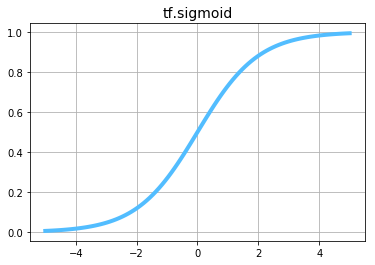
\includegraphics[width=0.65\textwidth]{./sync_imgs/act/smooth/sigmoid.png}
	\label{fig:act_smooth_sigmoid}
\end{figure}

% {{{act_smooth_tangent}}}
\begin{figure}
	\centering
	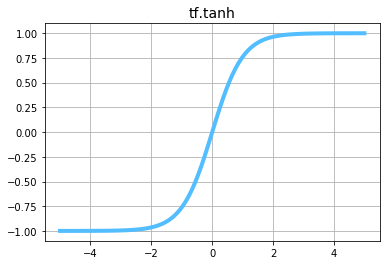
\includegraphics[width=0.65\textwidth]{./sync_imgs/act/smooth/tangent.png}
	\label{fig:act_smooth_tangent}
\end{figure}

\subparagraph{ELU}

\textcolor{blue}{\textcolor{red}{CITE}. Smooth, monotonic, and non-zero in the negative portion of the input. The main drawback is that they are more computationally expensive (due to calculating the exponential)}


\begin{equation}
{
	ELU = f(x) = \left\{
	\begin{array}{ll}
	\alpha(e^x - 1) x & \quad $for$ \ x < 0 \\
	x & \quad $for$ \ x \ge 0
	\end{array}
	\right.
}
\label{eq:act_elu_def}
\end{equation}


% {{{act_smooth_elu}}}
\begin{figure}
	\centering
	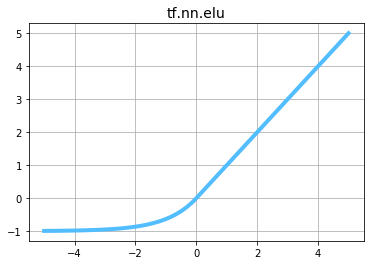
\includegraphics[width=0.65\textwidth]{./sync_imgs/act/smooth/elu.png}
	\label{fig:act_smooth_elu}
\end{figure}

% {{{act_smooth_selu}}}
\begin{figure}
	\centering
	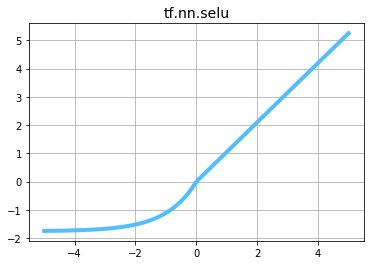
\includegraphics[width=0.65\textwidth]{./sync_imgs/act/smooth/selu.png}
	\label{fig:act_smooth_selu}
\end{figure}


\subparagraph{Softplus}

\textcolor{blue}{continuous and differentiable at zero. However, due to the natural log and exponential function, there is added computation compared to th ReLU.}

% typcially discouraged in practice since ReLU achieves similar results and is less computationally expensive

\begin{equation}
{
	Softplus = f(x) = \ln{(1+e^x)}
}
\label{eq:act_softplus_def}
\end{equation}


% {{{act_smooth_softplus}}}
\begin{figure}
	\centering
	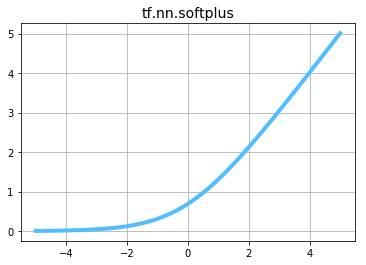
\includegraphics[width=0.65\textwidth]{./sync_imgs/act/smooth/softplus.png}
	\label{fig:act_smooth_softplus}
\end{figure}

% {{{act_smooth_softsign}}}
\begin{figure}
	\centering
	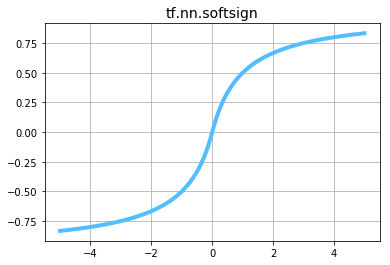
\includegraphics[width=0.65\textwidth]{./sync_imgs/act/smooth/softsign.png}
	\label{fig:act_smooth_softsign}
\end{figure}


\paragraph{Not Smooth Non-linear}

\subparagraph{ReLU}

\begin{equation}
{
	ReLU = f(x) = \left\{
	\begin{array}{ll}
	0 & \quad $for$ \ x < 0 \\
	x & \quad $for$ \ x \ge 0
	\end{array}
	\right.
}
\label{eq:act_relu_def}
\end{equation}

% {{{act_notsmooth_relu}}}
\begin{figure}
	\centering
	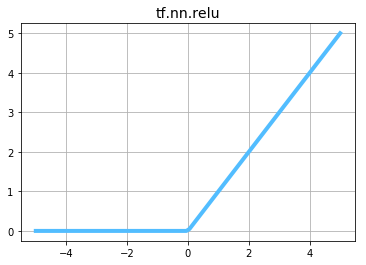
\includegraphics[width=0.65\textwidth]{./sync_imgs/act/notsmooth/relu.png}
	\label{fig:act_notsmooth_relu}
\end{figure}

\subparagraph{Leaky ReLU}

\textcolor{blue}{The Leaky ReLU (Eq~\ref{eq:act_leaky_relu_def}) was designed in attempt to address the dying ReLU issue \textcolor{red}{CITE}. Rather than simply outputting a zero in the negative range, the Leaky ReLU will will have a small non-zero slope (user specified) -- allowing weight updating and training to continue.}

\textcolor{green}{TODO: randomized Leaky ReLU \textcolor{red}{cite} --- $\alpha$ (from PReLU) is sampled from a uniform distribution randomly. The net-effect could be considered similar to drop out since, technically, there is a different network for each value of $\alpha$, resulting in an ensemble of sorts. At test time, the values for $\alpha$ are averaged.}

\begin{equ}[!ht]
	\begin{equation}
	{
		Leaky ReLU = f(x) = \left\{
		\begin{array}{ll}
		N x & \quad $for$ \ x < 0 \\
		x & \quad $for$ \ x \ge 0
		\end{array}
		\right.
	}
	\label{eq:act_leaky_relu_def}
	\end{equation}
	\caption{where $N$ is a constant. $N$ is typically set to 0.01}
\end{equ}

% {{{act_notsmooth_leakyrelu}}}
\begin{figure}
	\centering
	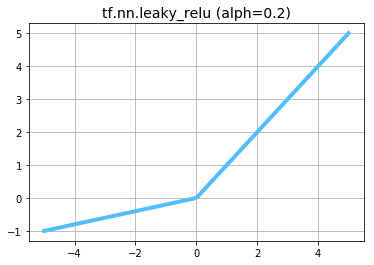
\includegraphics[width=0.65\textwidth]{./sync_imgs/act/notsmooth/leakyrelu.png}
	\label{fig:act_notsmooth_leakyrelu}
\end{figure}

\subparagraph{ReLU6}

\textcolor{blue}{In general, this function is referred to as a {ReLUN}\index{ReLUN} function, where $N$ is some constant. However, in practice, $6$, was determined to be the optimal value.\textcolor{red}{CITE}. \textcolor{red}{This capped value, may help learn the sparse values sooner.} By having the upper limit bounded, the prepare the network for a fixed point precision for inference --- if the upper limit is unbounded, then you may loose too many bits to \textcolor{red}{Q} portion of the fixed point number.}


\textcolor{blue}{Similar to the ReLU fuction, only the output is capped to six in the positive domain.}

\begin{equation}
{
	ReLU6 = f(x) = min{(max{(0,x)},6)}
}
\label{eq:act_ReLU6_def}
\end{equation}

% {{{act_notsmooth_relu6}}}
\begin{figure}
	\centering
	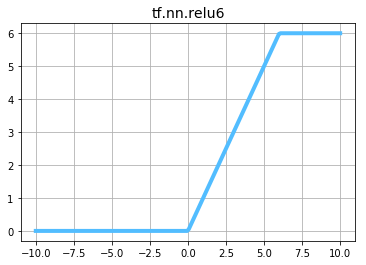
\includegraphics[width=0.65\textwidth]{./sync_imgs/act/notsmooth/relu6.png}
	\label{fig:act_notsmooth_relu6}
\end{figure}

\subparagraph{PReLU}

\begin{equ}[!ht]
	\begin{equation}
	{
		PReLU = f(x) = \left\{
		\begin{array}{ll}
		\alpha x & \quad $for$ \ x < 0 \\
		x & \quad $for$ \ x \ge 0
		\end{array}
		\right.
	}
	\label{eq:act_prelu_def}
	\end{equation}
	\caption{where $\alpha$ is a parameterized --- a learned parameter from training.}
\end{equ}

\r{Parametric Rectified Linear Unit (PReLU) \cite{he2015delving}}

\textcolor{blue}{$\alpha$, rather than being hard coded, is determined during training by the data. The logic being that the value would be more optimal than we could set \textcolor{red}{CITE}}

% {{{act_notsmooth_prelu}}}
\begin{figure}
	\centering
	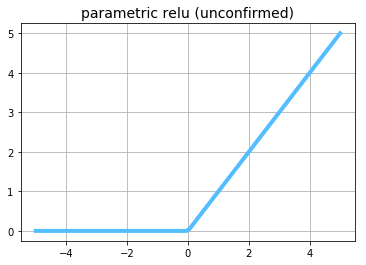
\includegraphics[width=0.65\textwidth]{./sync_imgs/act/notsmooth/prelu.png}
	\label{fig:act_notsmooth_prelu}
\end{figure}







%%%%%%%%%%%%%%%%


\subsection{Characterization}

\subsubsection{Types: Feed-forward vs Feedback}

\textcolor{blue}{Feed-forward --- Directed acyclic graph of artificial neurons. Feedback contain feedback connections that are fed back into itself. When feedforward are include these feedback connections, they become considered recurrent neural networks.}

\paragraph{Feed-forward}

\r{``general framework for representing non-linear functional mappings between a set of input variables and a set of output variables''}

\subparagraph{Layered networks}

\begin{figure}[htp]
	\centering
	\includegraphics[width=0.5\textwidth]{example-image-a}\hfil
	\caption{\TD{TODO: layered network diagram}}
	\label{fig:foundations_ann_layered_network}
\end{figure}

\r{Whereas a single layer network is composed of linear combination of input variables, that are then, transformed by a non-linear activation function, more general functions are creating layered networks that are composed of successive layers of processing units (adaptive weights) with connections running from every unit in one layer to every unit in the next.}

\subparagraph{General topologies}

\begin{figure}[htp]
	\centering
	\includegraphics[width=0.5\textwidth]{example-image-b}\hfil
	\caption{\TD{TODO: general topology}}
	\label{fig:foundations_ann_general_topology}
\end{figure}

\r{general topologies}

\paragraph{Feedback}

\subsubsection{Terminology}

\r{Considered \textit{networks} since they are typically composed of many different functions --- creating a ``network''.}

\r{Considered \textit{neural} since they are \textbf{loosely} inspired by neuroscience.}

\r{layer --- a layer may be considered a group of units that act in parallel. The layer will extract representations from the input, that are (in theory) more useful to the specific task.  Chaining together these layers results in a form of progressive \IDI{data distillation}.}

\r{Visible and Hidden Layers. Visible layers are called visible since they contain variables that are ``visible'', where as the hidden layers extract increasingly abstract features -- hidden since their values are not given in the raw data, but rather an output from a previous layer.}



\subsection{Learning: Backpropagation}

% see p196[184] of Mastering ML w/SKL
\TD{TODO: whoooo, this is going to be a big one. understand how each component contributes to the error and adjust accordingly.}

\r{popularized by \TD{Rumelhard, Hinton and Williams (1986)}, but similar ideas were discussed earlier by \TD{Werbos 1974}, and \TD{Parker 1985}}

\r{error backpropagation is used for evaluating the dervivatives of an error function with respect to the parameters (weights and biases) of the network}

\r{Iterative algorithm consisting of two main components --- the forward, then reverse, pass.}

% see p.141(156) - 146(161) of NNbishop
\TD{MORE}

\TD{Example}

\paragraph{Forward pass}

\r{In the forward pass inputs are propagated through the network and derivatives of the error functuion, with respect to the parameters (weights and biases) are evaluated. Propagation o ferrors through the network, calculating the derivatives, can be applied to may different error functions.}

\r{it becomes important to use a computationally efficient method for evaluating these derivatives \TD{local ref}}

\r{During this stage is when the errors are propagated through the network.}

\paragraph{Backward pass}

\r{In the Backward pass, the previously calcuated derivatives are used to compute the adjustments to the parameters --- propagated in reverse through the network (from cost function to input layer) and each node is updated -- \TD{TODO: expand}.}

\r{Many optimization schemes \TD{local ref} may be used to adjust the parameters by using the calculated derivatives from the forward pass.}

\r{The calculated derivatives are used by the majority of training algorithms}

%% p116 of neural networks, p131 on tablet
\TD{Hessian matrix is a matrix containing the second derivative of a function. The second derivative provides information about the curvature of the function.}

% see p197-201[180] of Mastering ML w/SKL
\TD{TODO: figure showing sample calculation}


% See p207 of DL

\r{also sometimes called \IDI{reverse-mode differentiation}.  Calculate the contribution that each parameter had on the loss value}

\r{\IDI{symbolic differentiation} --- compute a gradient function for the chain (chain rule) mapping parameter values to gradient values}

\subsubsection{Back-propagation efficiency}

%% see para in p146(161) of bishop NN

\subsubsection{Chain Rule}

\r{See \textcolor{red}{local ref to math prereq section}}

\TD{TODO: chain rule}

\r{Backpropagation is typically used with an optimization algorithm (see \textcolor{red}{local ref?})}

\subsection{Multi-layer perceptrons}

% TODO: this doesn't really belong here.. will need ot work on placement

\subsection{Operations}

\subsection{Convolution}
% TODO: I'm not sure how I'm going to structure these yet or where I'll be placing them

% TODO: https://arxiv.org/abs/1904.11486
% https://www.youtube.com/watch?v=HjewNBZz00w


\r{really when we refer to the convolution opperation, we are lying and actually refering to the cross-correlation, since we don't rotate the kernel 180$\deg$.}


% Graham Taylor
\r{weighted averaging operation in time or space}

\r{translational invariant --- if a feature is learned in one corner, it can be observed in another area as well.}

\r{translation equivariant --- }

\r{DNN on an image may not take advantage of the ``stationarity'' (statistics) of an image. Patterns don't depend on the spatial location.}

\r{spatial hierarchies --- \TD{TODO: figure raw data, abstract edges+, then more distinct images, then closer output to the output, then the final label}}

\textcolor{red}{local ref to TensorFlow implementation}

\r{typcially a feature extraction phase (consisting of convolutional and pooling layers) followed by a classifier block (dense layers).}

%%%% popular layer types
\textcolor{green}{TODO: feature maps, (height, width, and depth (also called channels axis)). Stride, filter size, depth. talk about parameters}

\r{The output feature map (every dimension in the depth axis is a feature/filter) --- after a convolution operation the depth of a layer is no longer representative of a color channel (like RGB), it is now representative of a feature extracted by the convolutional operation, these are called filters.}

\TD{Strided Convolution\cite{springenberg2014striving}}

\TD{Dilated Convolution --- `atrous' convolution. (famously used by wavenet), which is convenient in time series analysis.}

\r{weight tieing}


\textcolor{green}{TODO: figure}

\begin{figure}[htp]
	\centering
	\includegraphics[width=0.5\textwidth]{example-image-a}\hfil
	\caption{Figure example of convolution operation on 2d image \textcolor{green}{TODO}}
	\label{fig:conv_2d_example_calc}
\end{figure}

\begin{figure}[htp]
	\centering
	\includegraphics[width=0.5\textwidth]{example-image-b}\hfil
	\caption{Figure example of convolution operation on 3d image \textcolor{green}{TODO}}
	\label{fig:conv_2d_depth_example_calc}
\end{figure}

\textcolor{green}{TODO: examples of how different filter values and strides can effect the output dimensions.}




\subsection{Pooling}
% TODO: I'm not sure how I'm going to structure these yet or where I'll be placing them -- pooling really does not belong under feed forward

\TD{TODO: examples of max vs average pooling}

%%%%%% research
\textcolor{blue}{Pooling may not fully determine learned deformation stability -- possibly filter smoothness\cite{ruderman2018learned}}

\r{downsampling}

\r{Why? importance of reducing the number of params.}

\TD{L2-pooling}

\TD{L2-pooling over the features or channels.}

\TD{additional --- learned/parameterized pooling}

\begin{figure}[htp]
	\centering
	\includegraphics[width=0.5\textwidth]{example-image-a}\hfil
	\caption{Figure example of max pooling operation on 2d image \textcolor{green}{TODO: I want this figure to be basic 2d}}
	\label{fig:pooling_max_2d_ex_a}
\end{figure}

\begin{figure}[htp]
	\centering
	\includegraphics[width=0.5\textwidth]{example-image-b}\hfil
	\caption{Figure example of average pooling operation on 3d image \textcolor{green}{TODO: I want this figure to be 3d}}
	\label{fig:pooling_avg_3d_ex_a}
\end{figure}


\r{may be better to use convolutional layers in place of the pooling layers\cite{springenberg2014striving}}

%%%%%%%%%%%%%%%%%%%%%%%%%%%%%% feedforward
\section{Feed-forward}

\textcolor{blue}{A feedforward network can be represented as a directed acyclic graph -- a directed graph in which there exist no cycles in the underlying graph, with nodes representing neurons and connected by edges}

\textcolor{blue}{layer depths ~ to hierarchy of features}




%%%% popular layer types

\textcolor{blue}{convolution}

\textcolor{blue}{capsule}


%%%%%%%%%%%%%%%%%%%%%%%%%%%%%% feedback
\section{Feedback or Recurrent}

\textcolor{green}{TODO: Overview}

%%%% popular layer types

\textcolor{blue}{LSTM}

\textcolor{blue}{GRU}

\r{RNNs or ``\textit{\textbf{r}}ecurrent \textit{\textbf{n}}eural \textit{\textbf{n}}etworks'' are used for a variety of purposes but are typically designed with sequences of data as an input in mind. They are similarin concept to a standard/feed-forward netowrk, with the major distinction being that they also have connections that point ``backwards'' i.e. they have connections that feed into themselves.}

\r{Are capable fo working on sequences of arbitrary lengths, rather than fixed-sized inputs}

\subsection{Foundation}

\r{An example of an RNN diagram is shown in \TD{fig}. However, this representation is misleading since it does not show ``every'' connection in the model --- most notably, the recurrent connections.  RNNs may also be often represented in diagrams as ``unrolled'' (\TD{fig}). The unrolled RNN is easier to visualize how these recurrent connections are included.  This makes it easier to understand how each timestep is dependent on not only the current input (at the particular time step), but also dependent on ``all'' previous time steps. It is often stated that at a certain timestep (n), the output has ``memory'' since it is a function of all the previous time steps.}


\footnotetext{the term ``all'' is emphasized here since it is the goal to include information from all previous time steps. This is true in theory, however, this is not always the case in practice. This is discussed further in \ALR{}}

\subsection{Simple RNN and Recurrent Neuron}

\TD{Diagram of the inside of a RNN neuron}


\subparagraph{Overview}

\TD{todo}


\section{Common Problems}

Two well known main problems with RNNs.

\begin{enumerate}[noitemsep,topsep=0pt]
	\item Maintaining states are expensive
	\item Vanishing and/or exploding gradients
\end{enumerate}

\TD{hardware acceleration}

\subsection{Maintaining States}


\subsection{Addressing Vanishing and Exploding Gradients}

\r{Propagating signals through a long/deep network without loosing (vanishing gradient) or overamplifying the signal (exploding gradient) is difficult.  There have been a few advances to address this issue.}

\begin{enumerate}[noitemsep,topsep=0pt]
	\item Architecture (different cell types, memory schemes)
	\item Initialization Strategies
	\item Activation Function
\end{enumerate}




\section{Architecture}

\TD{a different section focusing on this}



\subsection{Cell Advancements}

\subsubsection{LSTM}

Introduced in 1997 %\cite{hochreiter1997long}

\r{detect long term dependencies in sequence}

\r{two state vectors, short and long term}

\r{Main motivation: learning what to store in the long-term state and what to ``forget''.}

\r{at each time step, some information is ``stored'' and some information is ``forgotten''.}

\paragraph{Fully Connected Layers}


\begin{enumerate}[noitemsep,topsep=0pt]
	\item Main
	\item \textit{Gate Controllers}
	\begin{enumerate}[noitemsep,topsep=0pt]
		\item Forget
		\item Input
		\item Output
	\end{enumerate}
\end{enumerate}

\r{The gate controllers use a logistic activation fuction (output a range from 0 to 1). This output is then fed through an element-wise multiplication function and thus if the value is $0$, the gate is ``closed'', and $1$ if the gate is ``open''.}

\r{These gates are able to potentially:}

\begin{enumerate}[noitemsep,topsep=0pt]
	\item Recognize an important input
	\item Store the important input in a long-term state ()
	\item Preserve the information for as long as it's needed
	\item Extract the important information when needed
\end{enumerate}


\subparagraph{Main}

\begin{figure}
	\centering
	\includegraphics[width=0.5\textwidth]{example-image-a}\hfil
	\caption{\TD{Main Layer DIAGRAM}}
	%\label{}
\end{figure}

\r{This allows for the same basic functionality as a ``standard'' RNN cell --- however, the output, rather than being only sent to the next cell, is now partially stored in the long-term state.}


\subparagraph{Forget}

\r{Determines which part of the long-term state is forgotten/erased.}

\begin{figure}
	\centering
	\includegraphics[width=0.5\textwidth]{example-image-a}\hfil
	\caption{\TD{Forget Layer DIAGRAM}}
	%\label{}
\end{figure}



\subparagraph{Input}

\r{Determines which part of the output from the \textbf{main layer} are kept in the long-term state.}

\begin{figure}
	\centering
	\includegraphics[width=0.5\textwidth]{example-image-a}\hfil
	\caption{\TD{Input Layer DIAGRAM}}
	%\label{}
\end{figure}

\subparagraph{Output}

\r{Determines which part of the long term state is ``relevant'' (read and output).}

\begin{figure}
	\centering
	\includegraphics[width=0.5\textwidth]{example-image-a}\hfil
	\caption{\TD{Output Layer DIAGRAM}}
	%\label{}
\end{figure}


\paragraph{Other}

\subparagraph{Peephole Connections}

\r{In basic LSTM cells, the gate controller can only look at the input and previous short-term state. Peephole connections, proposed in 2000 \TD{cite gers2000recurrent} add an extra connection that allows for the gate controller to also see information from the long term state as well. }

\r{The previous long-term state also becomes an input to the forget and input gate. The current long-term state becomes an intput to the output gate.}



\subsubsection{GRU}

\r{The GRU (gated recurrent unit) is a varient of the LSTM cell \TD{cite - cho2014learning}. The main modifications include:}

\begin{itemize}[noitemsep,topsep=0pt]
	\item Both state vectors are merged into one state vector
	\item A single gate controller determines the \textbf{Forget} and \textbf{Input} gate
	\begin{itemize}[noitemsep,topsep=0pt]
		\item If the gate output is a 1, the input is open and the forget gate is closed. If the gate output is 0, the input gate is closed and the forget gate is open
	\end{itemize}
	\item \r{The output gate is removed and a new controller exists that controls which part of ht previous state will be ``shown'' to the main layer}. At each timestep the full state vector is output.
\end{itemize}



\subsection{Initialization}

\subsection{Activation Functions}

\subsection{Notes -- add}

\r{A recent paper \TD{greff2017lstm}, comares three LSTM variants and makes three main observations:}

\begin{itemize}[noitemsep,topsep=0pt]
	\item no significant architecture improvements over LSTMs
	\item forget gate and the output activation function are the most critical components
	\item \TD{hyperparams...}
\end{itemize}












\chapter{Common Operations}

\chapter{Overview}

% TODO: this chapter needs serious restructuring/organization consideration

\section{Introduction}

\textcolor{green}{TODO: Tensorflow is an open-source library for numerical computation (not only as a deep/machine learning framework), released by google XXXXXXXXX.}

\textcolor{green}{TODO: There are many different deep learning frameworks}

\textcolor{green}{TODO: why use a deep learning framework}

\section{High-level Overview of Components}

\textcolor{green}{TODO: paras with local refs to components}

\textcolor{green}{TODO: Diagram of tensorflow at a high level}


\section{TensorFlow Essentials}

\subsection{API Hierarchy}

\subsection{Placeholders, feed\_dict, Variables and Constants}

\textcolor{blue}{using get\_variable to create the variable}

\subsection{Coding Style}

\textcolor{blue}{Imperative vs lazy evaluation.}

\subsection{Graphs}

\textcolor{blue}{TODO: Graphs.}

\textcolor{blue}{directed}

\textcolor{blue}{acyclic}

\textcolor{blue}{Why directed acyclic graph (DAG) representation? Language and Hardware Portability -- Developers get to develop programs in a high level language (like python) and have the TensorFlow execution engine execute (written in C++) the model on different platforms (targeted for exact hardware)}

\subsection{Sessions}

\textcolor{blue}{TODO: Sessions.}

\subsection{Tensors}

\textcolor{blue}{TODO: what is a tensor. Tensor --- an n dimensional array of data. they ``flow" through the (directed, acyclic) graph --- hence, TensorFlow}

\section{Workflow}

\textcolor{green}{TODO: Diagram of a typical workflow}

% lazy evaluation
\textcolor{blue}{first step is to build the graph, the second step is to execute the graph (in a session, which will evaluate to numpy arrays)}

% eager mention
\textcolor{blue}{There exists another mode of operation called ``eager'', in which the operations are executed imperatively (tf.eager is discussed in further detail in \textcolor{red}{local ref})}

\textcolor{blue}{TODO: list of overloaded operations, common arithmetic operators/shorthand}

% TODO: this belongs somewhere else
\textcolor{blue}{Note about how training is more computationally expensive than inference}

\section{Debugging TensorFlow}

\textcolor{blue}{Before writing any TensorFlow, I'd like to share some tips and tools to debug TensorFlow programs.}


\textcolor{blue}{error messages are your friend. Use the error message to isolate and debug the operation that is causing problems.}

\textcolor{blue}{two pieces of information: i) stack trace and ii) error message (type+message and operation) }

\subsection{Common Errors}
% tensor shape
% scalar-vector mismatch
\subsubsection{Shape}

% TODO: show how to use these common operations and their output
\textcolor{blue}{some common operations to change the shape of a tensor may included i) tf.reshape() ii) tf.expand\_dims(), iii) tf.slice(), and iv) tf.squeeze() --- expand and squeeze are inverses} 

\subsubsection{Data Type}
% data type mismatch

\subsection{Debugging Tools}

\subsubsection{tf.Print}
% log specific tensor values
%TODO: Code Examples

\subsubsection{tfdbg}

%TODO: Code Examples

% python super_tf_model.py --debug

\subsubsection{TensorBoard}

%TODO: diagram examples

\textcolor{blue}{Using TensorBoard for monitoring is discussed in a later section(\textcolor{red}{local ref}). The scope in this section will focus on using TensorBoard to debug a program}

\subsubsection{Logging and Verbosity}

% different modes overview debug --> fatal
% info = development, warn = production
% tf.logging.set_verbosity(tf.logging.INFO)







\chapter{Applied Neural Networks}

\chapter{Overview}

% TODO: this chapter needs serious restructuring/organization consideration

\section{Introduction}

\textcolor{green}{TODO: Tensorflow is an open-source library for numerical computation (not only as a deep/machine learning framework), released by google XXXXXXXXX.}

\textcolor{green}{TODO: There are many different deep learning frameworks}

\textcolor{green}{TODO: why use a deep learning framework}

\section{High-level Overview of Components}

\textcolor{green}{TODO: paras with local refs to components}

\textcolor{green}{TODO: Diagram of tensorflow at a high level}


\section{TensorFlow Essentials}

\subsection{API Hierarchy}

\subsection{Placeholders, feed\_dict, Variables and Constants}

\textcolor{blue}{using get\_variable to create the variable}

\subsection{Coding Style}

\textcolor{blue}{Imperative vs lazy evaluation.}

\subsection{Graphs}

\textcolor{blue}{TODO: Graphs.}

\textcolor{blue}{directed}

\textcolor{blue}{acyclic}

\textcolor{blue}{Why directed acyclic graph (DAG) representation? Language and Hardware Portability -- Developers get to develop programs in a high level language (like python) and have the TensorFlow execution engine execute (written in C++) the model on different platforms (targeted for exact hardware)}

\subsection{Sessions}

\textcolor{blue}{TODO: Sessions.}

\subsection{Tensors}

\textcolor{blue}{TODO: what is a tensor. Tensor --- an n dimensional array of data. they ``flow" through the (directed, acyclic) graph --- hence, TensorFlow}

\section{Workflow}

\textcolor{green}{TODO: Diagram of a typical workflow}

% lazy evaluation
\textcolor{blue}{first step is to build the graph, the second step is to execute the graph (in a session, which will evaluate to numpy arrays)}

% eager mention
\textcolor{blue}{There exists another mode of operation called ``eager'', in which the operations are executed imperatively (tf.eager is discussed in further detail in \textcolor{red}{local ref})}

\textcolor{blue}{TODO: list of overloaded operations, common arithmetic operators/shorthand}

% TODO: this belongs somewhere else
\textcolor{blue}{Note about how training is more computationally expensive than inference}

\section{Debugging TensorFlow}

\textcolor{blue}{Before writing any TensorFlow, I'd like to share some tips and tools to debug TensorFlow programs.}


\textcolor{blue}{error messages are your friend. Use the error message to isolate and debug the operation that is causing problems.}

\textcolor{blue}{two pieces of information: i) stack trace and ii) error message (type+message and operation) }

\subsection{Common Errors}
% tensor shape
% scalar-vector mismatch
\subsubsection{Shape}

% TODO: show how to use these common operations and their output
\textcolor{blue}{some common operations to change the shape of a tensor may included i) tf.reshape() ii) tf.expand\_dims(), iii) tf.slice(), and iv) tf.squeeze() --- expand and squeeze are inverses} 

\subsubsection{Data Type}
% data type mismatch

\subsection{Debugging Tools}

\subsubsection{tf.Print}
% log specific tensor values
%TODO: Code Examples

\subsubsection{tfdbg}

%TODO: Code Examples

% python super_tf_model.py --debug

\subsubsection{TensorBoard}

%TODO: diagram examples

\textcolor{blue}{Using TensorBoard for monitoring is discussed in a later section(\textcolor{red}{local ref}). The scope in this section will focus on using TensorBoard to debug a program}

\subsubsection{Logging and Verbosity}

% different modes overview debug --> fatal
% info = development, warn = production
% tf.logging.set_verbosity(tf.logging.INFO)








\chapter{Unsupervised}

\r{The reality is that data is not always labeled.}

\r{unsupervised learning is capable of finding hidden patterns in the underlying structure of hte data.}

\r{attempts to represent data with increaingly fewer parameters}

\textcolor{blue}{Discovering hidden structures or patterns in unlabeled training data.}

\TD{Neighborhood-Based Methods \ref{nearest_neighbors} \r{lazy learners  -- learn how to label new instances based on proximity to existing instances}}

% TODO: placement / may need to rename+restructure sections
\textcolor{blue}{unsupervised methods may be commonly used in two main settings:}
\begin{enumerate}[noitemsep,topsep=0pt]
	\item Data Exploration
	\begin{itemize}[noitemsep,topsep=0pt]
		\item Visualization (clustering \textcolor{red}{local ref})
	\end{itemize}
	\item Preprocessing (e.g. prior to a supervised method): unsupervised pretraining may be considered a form of regularization
	\begin{itemize}[noitemsep,topsep=0pt]
		\item Compressing (dimensionality reduction \textcolor{red}{local ref})
		\item Creating new/different representations
	\end{itemize}
\end{enumerate}

\r{regularization, feature engineering, detecting outliers -- also used for detecting how different new (incoming) training data is from the current distribution.}

\r{popular applications --- anomaly detection, group segmentation, preprocessing (dimensionality reduction)}

\subsection{TODO}

\TD{evaluating unsupervised learning systems are harder to evaluate than supervised learning systems.}

%%%%%%%%%%%%%%%%%%%%%%%%%%%%%% clustering
\section{Clustering}

\textcolor{blue}{Clustering, may be referred to as cluster analysis, involves grouping observations such that instances in the same group (cluster) are more similar to one another than they are to instances from another group --- where ``similarity'' is defined by `some metric'. Clustering may be used to explore a dataset}

\textcolor{blue}{Clustering may be used to perform {image quantization}\index{image quantization}, a lossy compression methods that will replace similar colors with a single color to reduce the size of the image file.}

\r{Finding sub groups where observations are more similar to eachother based on some similarity measure. Clustering is sometimes referred to as ``unsupervised classification'' and is often used to explore a dataset.}

\r{An example of clustering may be to group a collection of documents into categories, or songs into genres. examples --- recommendation system}

\subsection{Common Algorithms}

\r{Major clustering algorithms}
\begin{itemize}[noitemsep,topsep=0pt]
	\item k-means
	\item hierarchical clustering
	\item DBSCAN
\end{itemize}

\subsubsection{K-means}

\r{iterative process -- moves centroid (center of cluster) to mean position of instances then reassigning instances to clusters by closest centroid}

\r{will continue to iterate until some stopping criteria is satisfied.}

\r{To avoid unlucky initialization leading to convergence on local optima, K-means may be repeated many times (dozens to hundreds) with a random initialization. The initialization values that lead to the minimum cost function is then determined to be best.}

\r{$k$ (positive integer less than the number of instances in the training set) specifies the number of clusters/centroids}

\r{minimizes the within-cluster/group variation (also known as the initeria)}

\r{the more clusters, the initeria decreases}

\TD{TODO: k-means cost function}

\r{important to note that K-means will not necessarily converge on the global optimum. Different runs will result in slightly different cluster assignments.}

\r{randomly assigns each observation to one of the k clusters}

\r{reassigns obervations in order to minimize the Euclidean distance between the observation and cluster's center.}

\r{several runs -- lowest total sum of within-cluster variation}

\TD{TODO: variations such as mini-batch k-means}

\r{}

\paragraph{Local Optima}

\textcolor{blue}{unlucky initialization}

\paragraph{Selecting K}

\TD{todo: Overview}

\r{No right/theoretical answer, need to perform trial and error: optimal number found by minimizing the cost function}

\paragraph{Elbow Method}

\textcolor{blue}{The elbow method is used to select the optimal number of clusters if $k$ is not specified by the problems context.}

% rough
\textcolor{blue}{plot of the final cost function value is plotted against the value of $k$. As $k$ increases, the average distortion will decrease as each cluster will have fewer instances and they will be closer to their respective centroid. This decline in dispersion will decline most at a point and then slowly continue to decline -- the point at which the dispersion decreases the most can be considered the elbow (and considered by the elbow method to be the best value for $k$)}

\textcolor{green}{TODO: diagram showing data clusters}

\textcolor{green}{TODO: diagram showing $k$ vs dispersion related to above cluster diagram}



\subsubsection{Hierarchical Clustering}

\TD{overview}

\TD{agglomerative --- tree-based clustering that builds a dendogram --- upside-down tree}

\r{after evaluation, the user can decide which size of tree tey want to use.}

\r{by default Euclidian distance is used, but other similarity metrics can also be used \TD{link to reference}}

\TD{figure example}

% TODO: this likely diens't fit here
\TD{Ward --- Ward's minimum variance method}

\subsubsection{DBSCAN}

\TD{\textbf{D}ensity-\textbf{b}ased \textbf{s}patial \textbf{c}lustering of \textbf{a}pplications with \textbf{n}oise.}

\r{user defined: minimum number of instances and distance}

\r{any instance that is not within a specified distance is labeled as an outlier}

\r{arbitrarily shaped clusters}

\subsubsection{HDBSCAN}

\r{Hierarchical DBSCAN --- groups on density then uses distance measure on the created groups iteratively}


\subsection{Evaluating}

\textcolor{blue}{There are no labels - can still evaluate using intrinsic measures}

\textcolor{blue}{measuring distortion of clusters}

\subsubsection{Silhouette Coefficient}

\textcolor{blue}{The {silhouette coefficient}\index{silhouette coefficient} is a measure of compactness and separation of clusters. The silhoette coefficient is calculated per instance or for a set of instances (where the value is calculated to be the mean of the individual instances in the group). Eq.\ref{eq:silhouette_coef_def} can be used to calculate the silhouette per instance, where $d$ is the mean distance between the instance and the instances in the next closest cluster and $b$ is hte mean distance between the instances in the indicated cluster.}

\begin{equation}
{s = \frac{db}{max(d,b)}}
\label{eq:silhouette_coef_def}
\end{equation}







%%%%%%%%%%%%%%%%%%%%%%%%%%%%%% Dimensionality Reduction
\section{Dimensionality Reduction}
\label{unsupervised_dimensionality_reduction}

\r{Dimensionality reduction is typically used to reduce the dimensions in a feature representation while retaining as much information as possible.}

\r{reproduce the orginal dataset from teh reduced feature set as well as possible.}

\r{Motivation: i) mitigate issues caused by the curse of dimensionality ii) compress data iii) visualize and explore datasets and improve interpretability -- interpreting data in high dimensions is harder than in lower dimension spaces (particularly three or less). May also be used to compress data before being used by another learning algorithm.}

\r{Example --- projecting 3D data into a 2D space.}

\r{project the raw high-dimensuional input data into  a lower-dimensional space by only \TD{iteratively removing the least explainatory dimensions.}}

\TD{Two major branches of dimensionality --- linear and nonlinear (manifold). The difference is in the projection, one is linear and the other is, you guessed it, nonlinear.}

\r{Unsupervised Transformations --- Dimensionality Reduction --- where the goal is to reduce the dimensionality of the data while retaining as much as the relevant information as possible}

%% topic extraction

\r{A high number of features may be computationally costly. Ability to generalize may be reduced if some of the features capture noise or are irrelevant to the underlying relationship. The goal could be to find the features that account for the greatest changes in the response variable}

\subsection{Principal Component Analysis}

\textcolor{green}{{Principal Component Analysis (PCA)}\index{Principal Component Analysis (PCA)} may also be known as the {Karhunen-Love Transform (KLM)}\index{Karhunen-Love Transform (KLM)} }

\textcolor{red}{eigen-decomposition of the covariance matrix}

%p232[220] of Masstering ML w/SKL
\textcolor{red}{``PCA is most useful whe 'the variance of the dataset is distributed unevenly across the dimensions'' }

% TODO: get var/covar defs (currently in regression tex)
\textcolor{blue}{carvariances between each par of dimensions in a dataset are described in a {covarience matrix}\index{covarience matrix} }

\r{combine highly correlated features -- represent with fewer (linearly uncorrelated) features}

\r{searches for linear combinations in all input variables --- retains as much of the variation (salient information) as possible (some is lost)}

\TD{several variants --- incremental PCA, nonlinear (kernel PCA), sparse (sparse PCA)}

\TD{NOTE: it is important to ensure the features are on the same scale before performing PCA.}

\subsubsection{Linear}

\paragraph{Incremental PCA}

\r{small batches.}

\paragraph{Sparse PCA}

\TD{generates PCs slightly differently than normal PCA. Searches for linear combinations in only some of the input variables.}

\subsubsection{Nonlinear}

\paragraph{Kernel PCA}

\TD{more}

\r{similarity funciton (kernel method). Effective when the original feature set is not linear separable}

\TD{type of kernel}

\TD{kernel coefficient (gamma) -- \ALR -- popular radial basis function kernel}


\subsection{Singular value decomposition (SVD)}

\TD{TODO}

\TD{rank matrix}

\subsection{Random Projection}

\TD{TODO}

\textcolor{red}{Johnson-Lindenstrauss lemma}

\r{two versions: standard (gaussian random projection) and sparse (sparse random projection)}

\subsubsection{Gaussian Random Projection}

\r{linear projection}

\subsubsection{Sparse Random Projection}

\TD{TODO}

\section{Nonlinear dimensionality reduction}

%%%% % plus index - unsupervised method
% see p156 of DL for more
\TD{manifold learning (or nonlinear dimensionality reduction)--- {manifold}\index{manifold}, though having a more formal mathematical meaning, will be considered a connected region for our machine learning purposes. --- Nonlinear transormation. PCA and random projection project the data linearly from high to low dimension.}

\subsection{Isomap}

\TD{isomap -- type of manifold learning. estimates the geodesic or curved distance (rather than euclidean) between a point and its neighbors}

\r{relative to neighbors on a manifold \textcolor{red}{rather than a plane?}}

\subsection{Multidimensional Scaling (MDS)}

\TD{TODO}

\subsection{Locally Linear Embedding (LLE)}

\r{segments data into smaller components (neighborhoods), \textcolor{red}{models each component as a linear embedding}}

\r{preserves distance within neighborhoods}

\TD{TODO}

\subsection{t-Distributed Stochastic Neighbor Embedding (t-SNE)}

\TD{TODO}

\TD{t-distributed stochastic neighbor embedding (t-SNE) --- non-linear --- }


\r{two probability distributions, one over pairs of points in a high-dimensional space and another in a low dimensional space. minimizes the \TD{kullback-Leibler divergences} between these two probability distributions.}


\textcolor{red}{nonconvex cost function}

\r{different initializations will generate different results --- no stable solution}

\textcolor{red}{HELLO}

\section{Non-geometric, no distance metric}

\subsection{Dictionary Learning}

\TD{TODO}

\r{learns sparse representation of the original data}

\r{atoms --- vectors in the dictonary. vectors are binary vectors. instances are reconstructed as weighted sum of atoms. easily identify vectors with the most nonzero values}

\r{the dictionary can be undercomplete or overcomplete. undercomplete: atoms $<$ features in the original dataset, or overcomplete: atoms $>$ features in the original dataset.}

\TD{mini-batch version of dictionary learning}


\subsection{Independent Component Analysis (ICA)}

\TD{Separate blended signals into individual components (signal processing)}

\subsection{TODO: others}


% TODO: find a good text on this -- this should be an in depth section
% TODO: dataset for individual voices ina coffeehouse


\TD{Latent Dirichlet allocation}

\r{nonlinear --- multidimensional scaling (MDS), locally linear embedding (LLE), independent componenet analysis (ICA), t-distributed stochastic neighbor embedding (t-SNE), dictionary learning, random trees embedding}

\subsection{Autoencoders}
% TODO: this may not belong here

\TD{discussed more in depth in \ALR}

\r{encoder and decoder --- trained at once}

\r{May be described as a network that learns an approximation of an identity function. reconstructs original features --- hidden layers, reduce parameters (forced to learn salient features), subsequent layers learn increasingly complex relations from the preceeding layers.}

\r{if given too much capacity (``too'' many parameters), the autoencoder may (likely should) simply memorize the observations.}

\paragraph{Undercomplete vs Overcomplete}
\r{undercomplete --- if the constrain encoders output to fewer dimensions than the input}

\r{overcomplete --- when the encoders output dimensions are larger than the input dimensions. typically used in addition to a form of regularization.}

%\paragraph{Sparse vs Dense}



\subsection{Generative Adversarial Networks}
% TODO: this may not belong here

\r{described in more detail in \ref{generative_adversarial_network}}

\subsection{Hidden Markov Model}
% TODO: this may not belong here

\r{simple markov model -- states change stochastically. future states only depend on current state (not prior states)}

\r{Hidden Markov model -- learn propbable next state given what is known about hte sequence of previous states}


% TODO: format / other
%\input{./foundations/unsupervised/applications}


\chapter{Semi-supervised}

\section{Semi-Supervised}

\textcolor{green}{TODO: overview}

\subsection{Examples}

\textcolor{green}{TODO: Examples}


\chapter{Common Architectures}


\TD{Overview}

% TODO: I'm still not sure if I should divide this up by ``types'' of architectures or types of problems and the architectures used to solve them.. maybe both? unsure...


Images and Videos
\begin{itemize}[noitemsep,topsep=0pt]
	\item Classification
	\item Segmentation
	\begin{itemize}[noitemsep,topsep=0pt]
		\item Semantic segmentation (where we don't differentiate between instances)
		\item Instance segmentation
	\end{itemize}
	\item Object detection
\end{itemize}


\subsection{Spatial Data}

\r{types of problems -- spatial to spatial (1:1), spatial to sequence, spatial to value (single or multiple)}

\subsubsection{Convolutional Approaches}

% Survey on CNNs
% TODO: a lot here -- good read
\TD{A Survey of the Recent Architectures of Deep Convolutional Neural Networks \cite{DBLP:journals/corr/abs-1901-06032}}


\subsubsection{Image Classification}
% Graham Taylor talk
\r{alexnet, network-in-network, inception/google lenet (end with $1 \times 1 \times N_{classes}$ into a global average pooling layer), vggnet}

\r{Resnet (similar to highway networks) --- skip connections ``residual modual/block'' (dynamically adjusting depth) (others in this time: fractal nets, stochastic XXXX nets, where skip connections are shortcut paths)}

\r{DenseNet --- where these skip connections are taken to an extreme. also, concatenation, not summation}

\r{Squeeze and Excitation network --- adaptive recalibration of feature maps. \TD{TODO}}

% fit into an architecture ``timeline''
\TD{ResNeXt\cite{xie2017aggregated}}


\subsection{Object Detection}

\r{sliding window and use each window as input to a classifier. But the problem is that we need to apply the classifier to a huge number of locations and scales and aspect ratios. A potential solution to this problem is to use region proposals.}

\r{region proposals were introduced by R-CNN \TD{cite}, where conventional methods were used to propose regions for the CNN to classify. It's important to note that most regions are not square may need to be warped to be insert to the CNN}

\r{Bbox regression is also used --- how much to offset the region proposal.}


\r{fast R-CNN proposed regions by using the feature maps from a layer from a CNN that was previously trained (VGG or Resnet, for example). after identifying the regions, then crop-resize, then CNN over each region, then get output (class + bbox regression.)}

\r{faster r-cnn. Insert a region proposal network (RPN) to predict proposals from features --- in this architecture, there are actually four losses to jointly train 1) object/net RPN, 2) box/net RPN, 3) Class prediction, and 4) final bounding box score.}


\subsection{Segmentation}

\r{fully convolution --- dowsample to upsample: 1) efficency when using convs on smaller dimensional inputs 2) latent representation}

\r{CNN and RPN --- nice results \TD{cite}}

\r{mask R-CNN --- also used for pose prediction}

% code: https://github.com/facebookresearch/detectron2/tree/master/projects/PointRend
% blog: https://ai.facebook.com/blog/using-a-classical-rendering-technique-to-push-state-of-the-art-for-image-segmentation/
\TD{PointRend: Image Segmentation as Rendering \cite{Kirillov2019PointRendIS}}


\section{Text: Natural Language Processing}


\section{Structured data: Tablular}


\section{Other Common Architectures}


 % ML algorithm foundations

\chapter{Ensemble Methods}

%%%%%%%%%%%%%%%%%%%%%%%%%%%%%% Ensemble Methods
\chapter{Overview}

% TODO: this chapter needs serious restructuring/organization consideration

\section{Introduction}

\textcolor{green}{TODO: Tensorflow is an open-source library for numerical computation (not only as a deep/machine learning framework), released by google XXXXXXXXX.}

\textcolor{green}{TODO: There are many different deep learning frameworks}

\textcolor{green}{TODO: why use a deep learning framework}

\section{High-level Overview of Components}

\textcolor{green}{TODO: paras with local refs to components}

\textcolor{green}{TODO: Diagram of tensorflow at a high level}


\section{TensorFlow Essentials}

\subsection{API Hierarchy}

\subsection{Placeholders, feed\_dict, Variables and Constants}

\textcolor{blue}{using get\_variable to create the variable}

\subsection{Coding Style}

\textcolor{blue}{Imperative vs lazy evaluation.}

\subsection{Graphs}

\textcolor{blue}{TODO: Graphs.}

\textcolor{blue}{directed}

\textcolor{blue}{acyclic}

\textcolor{blue}{Why directed acyclic graph (DAG) representation? Language and Hardware Portability -- Developers get to develop programs in a high level language (like python) and have the TensorFlow execution engine execute (written in C++) the model on different platforms (targeted for exact hardware)}

\subsection{Sessions}

\textcolor{blue}{TODO: Sessions.}

\subsection{Tensors}

\textcolor{blue}{TODO: what is a tensor. Tensor --- an n dimensional array of data. they ``flow" through the (directed, acyclic) graph --- hence, TensorFlow}

\section{Workflow}

\textcolor{green}{TODO: Diagram of a typical workflow}

% lazy evaluation
\textcolor{blue}{first step is to build the graph, the second step is to execute the graph (in a session, which will evaluate to numpy arrays)}

% eager mention
\textcolor{blue}{There exists another mode of operation called ``eager'', in which the operations are executed imperatively (tf.eager is discussed in further detail in \textcolor{red}{local ref})}

\textcolor{blue}{TODO: list of overloaded operations, common arithmetic operators/shorthand}

% TODO: this belongs somewhere else
\textcolor{blue}{Note about how training is more computationally expensive than inference}

\section{Debugging TensorFlow}

\textcolor{blue}{Before writing any TensorFlow, I'd like to share some tips and tools to debug TensorFlow programs.}


\textcolor{blue}{error messages are your friend. Use the error message to isolate and debug the operation that is causing problems.}

\textcolor{blue}{two pieces of information: i) stack trace and ii) error message (type+message and operation) }

\subsection{Common Errors}
% tensor shape
% scalar-vector mismatch
\subsubsection{Shape}

% TODO: show how to use these common operations and their output
\textcolor{blue}{some common operations to change the shape of a tensor may included i) tf.reshape() ii) tf.expand\_dims(), iii) tf.slice(), and iv) tf.squeeze() --- expand and squeeze are inverses} 

\subsubsection{Data Type}
% data type mismatch

\subsection{Debugging Tools}

\subsubsection{tf.Print}
% log specific tensor values
%TODO: Code Examples

\subsubsection{tfdbg}

%TODO: Code Examples

% python super_tf_model.py --debug

\subsubsection{TensorBoard}

%TODO: diagram examples

\textcolor{blue}{Using TensorBoard for monitoring is discussed in a later section(\textcolor{red}{local ref}). The scope in this section will focus on using TensorBoard to debug a program}

\subsubsection{Logging and Verbosity}

% different modes overview debug --> fatal
% info = development, warn = production
% tf.logging.set_verbosity(tf.logging.INFO)







\chapter{Term dump}

\textcolor{green}{Terms that are important but haven't been placed in the document yet}

\emph{Collinearity} --- When two or more predictor variables are closely related to one another they are said to be collinear.

\emph{Curse of Dimensionality} --- \r{phenomenon where the feature space becomes increasingly sparse as the number of dimensions/features is increased -- trade off between the density of instances in the feature space and the number of dimensions (number of descriptive features) \r{including too many features can paradoxically, lead to worsening of performance.} \textcolor{green}{TODO: mentioned in paper Bellman 1961}}

\emph{dummy variable} ---


\emph{Population vs Sample} -- the population (usually denoted $N$) is the collection of all the items of interest in a study where as the sample is a subset of a population (usually denoted $n$). The numbers obtained when working with a population are called the `parameters' and the numbers obtained when working with a sample are a called `statistics'. \textcolor{blue}{a random sample is obtained when each member of the sample is chosen from the population by chance and accurately reflects the population}

\emph{$e$} --- \textcolor{blue}{Euler's numbers}

\subsection{Distributions}

\emph{Normal Distribution} --- \textcolor{blue}{Normal, or Guassian, distribution. Data is symmetrical where half the values are greater than the mean and half the values are less than the mean. The median, mode, and mean are all equal}

\emph{Bernoulli Distribution} --- \textcolor{blue}{distribution in which XXXXXXXXXXXX}

\emph{epoch} --- \textcolor{blue}{a complete pass through the entire training set.}

\emph{vector} --- \textcolor{blue}{direction, and magnitude (length)}

\emph{eigenvalue} and \emph{eigenvector} --- \textcolor{blue}{`eigen' is a german word for ``belonging to'' or ``particular to''.} 


\part{Brief Reference}



\textcolor{blue}{Brief overview of how all packages and environments work together.}

%%%%%%%%%%%% Environment
\chapter{Environment}

\textcolor{blue}{Overview of Environment}

\subsection{Terminal}

\section{Hardware}

\subsection{CPU vs GPU}

\subsection{Cloud Providers}

\subsection{AWS Quickstart}

\subsection{Python}

\textcolor{green}{TODO: overview}

\textcolor{blue}{This section will not teach you everything you need to know to be python programmer. Rather, this section will assume you have programming experience and will focus on a few of the components of python that may be frequently encountered and may benefit from further explanation and examples.}


\subsubsection{Datatypes}

\paragraph{Tuple}

\textcolor{blue}{fixed-length immutable sequence of Python objects.}

\paragraph{List}

\textcolor{blue}{variable-length mutable sequence of Python objects.}

\subparagraph{List Comprehensions}

\textcolor{blue}{para about list comprehensions}

% {{{py_nested_listcomp}}}
\begin{lstlisting}[style=pyInStyle]
matrix = [[1,2,3], [4,5,6], [7,8,9]]
# value is multiple of 3 and array sum >= 10
filtered = [[x for x in row if x % 3 == 0]
            for row in matrix if sum(row) >= 10]
print(filtered)
\end{lstlisting}
\begin{lstlisting}[style=pyOutStyle]
[[6], [9]]
\end{lstlisting}
\begin{markdown}
Using nested list comprehensions is possible but gets a little messy -- the rule of thumb is to not use more than 2 expressions in list comprehensions
\end{markdown}

\subparagraph{Append Vs Extend}

\textcolor{blue}{Append vs extend.}

% {{{py_app_v_ext}}}
\begin{lstlisting}[style=pyInStyle]
x = [1, 2, 3]
x.append([4, 5])
print("Append: {}".format(x))

x = [1, 2, 3]
x.extend([4, 5])
print("Extend: {}".format(x))
\end{lstlisting}
\begin{lstlisting}[style=pyOutStyle]
Append: [1, 2, 3, [4, 5]]
Extend: [1, 2, 3, 4, 5]
\end{lstlisting}


\paragraph{Dict}

\textcolor{blue}{para about dicts}

\paragraph{Set}

\textcolor{blue}{para about sets}

\subsubsection{Functions}

\textcolor{blue}{para about functions}

\paragraph{Keyword Only Arguments}

\textcolor{blue}{para about keyword only parameters}

% {{{py_func_kwonly}}}
\begin{lstlisting}[style=pyInStyle]
def func_with_kwargs(num, a, b,
                    *,
                    div_a=False,
                    div_b=False):
    if div_a:
        num /= a
    if div_b:
        num /= b
    return num

# print(func_with_kwargs(12, 2, 2, True, True)) # won't work
print(func_with_kwargs(12, 2, 2, div_a=True, div_b=True))
\end{lstlisting}
\begin{lstlisting}[style=pyOutStyle]
3.0
\end{lstlisting}
\begin{markdown}
all args after the `*` must be specified
\end{markdown}


\subparagraph{Optional Parameters}

\textcolor{blue}{para about optional parameters}

% {{{py_opt_params}}}
\begin{lstlisting}[style=pyInStyle]
def log(message, *values):
    if not values:
        print(message)
    else:
        val_str = ", ".join(str(x) for x in values)
        print("{}: {}".format(message, val_str))

log("current number")
log("current numbers are", 1, 2)
\end{lstlisting}
\begin{lstlisting}[style=pyOutStyle]
current number
current numbers are: 1, 2
\end{lstlisting}

\paragraph{Built-in Sequence Functions}

\subparagraph{enumerate}

\textcolor{blue}{Enumerate is used for ...}

% {{{py_enumerate_01}}}
\begin{lstlisting}[style=pyInStyle]
for i, letter in enumerate(["a", "b", "c", "d"]):
    print("letter[{}]={}".format(i, letter))
\end{lstlisting}
\begin{lstlisting}[style=pyOutStyle]
letter[0]=a
letter[1]=b
letter[2]=c
letter[3]=d
\end{lstlisting}


% {{{py_enumerate_02}}}
\begin{lstlisting}[style=pyInStyle]
for i, letter in enumerate(["a", "b", "c", "d"], 1):
    print("letter#{}={}".format(i, letter))
\end{lstlisting}
\begin{lstlisting}[style=pyOutStyle]
letter #1=a
letter #2=b
letter #3=c
letter #4=d
\end{lstlisting}
\begin{markdown}
Using nested list comprehensions is possible but tgets a little messy -- the rule of thumb is to not use more than 2 expressions in list comprehensions
\end{markdown}


\subparagraph{sorted}

\textcolor{blue}{para about sorted}

\subparagraph{zip}

\textcolor{blue}{para about zip}

% {{{py_zip}}}
\begin{lstlisting}[style=pyInStyle]
pets = ["Siren", "Diesel"]
age = [3, 2]
for pet_info in zip(pets, age):
    print(pet_info)
\end{lstlisting}
\begin{lstlisting}[style=pyOutStyle]
('Siren', 3)
('Diesel', 2)
\end{lstlisting}

% {{{py_zip_longest}}}
\begin{lstlisting}[style=pyInStyle]
pets = ["Siren", "Diesel", "Bella"]
age = [3, 2]
print("---- Using zip")
for pet_info in zip(pets, age):
    print(pet_info)

print("------ using zip_longest")
for pet_info in zip_longest(pets, age):
    print(pet_info)
\end{lstlisting}
\begin{lstlisting}[style=pyOutStyle]
---- Using zip
('Siren', 3)
('Diesel', 2)
------ using zip_longest
('Siren', 3)
('Diesel', 2)
('Bella', None)
\end{lstlisting}

\subparagraph{reversed}

\textcolor{blue}{para about reversed}

\subsubsection{Generators}

\textcolor{blue}{para about generators}

\subsubsection{Errors and Exception Handling}

\textcolor{blue}{para about errors and exception handling}

% {{{py_tryblock}}}
\begin{lstlisting}[style=pyInStyle]
try:
    # do something
except MyException as e:
    # handle exception
else:
    # runs when there are no exceptions
finally:
    # always runs after try:
\end{lstlisting}

\subsubsection{IO}

\textcolor{blue}{para about IO}

\subsubsection{Other}

\textcolor{blue}{para about other}

\textcolor{blue}{TODO: include note about broadcasting}




\section{git}

\subsection{Overview}

\subsection{Commands}

\subsection{Github}

\section{IDE}

\subsection{Atom}


\subsubsection{Installation}

Linux (Ubuntu) instructions from https://flight-manual.atom.io/getting-started/sections/installing-atom/. Two options: (i) install package repository on system, or (ii) download and install from `.deb'

\paragraph{(i) Package Repository}

First, add the official package repository to the system
\begin{lstlisting}[style=terminalBash]
curl -L https://packagecloud.io/AtomEditor/atom/gpgkey | sudo apt-key add -
sudo sh -c 'echo "deb [arch=amd64] https://packagecloud.io/AtomEditor/atom/any/ any main" > /etc/apt/sources.list.d/atom.list'
sudo apt-get update
\end{lstlisting}

Next, install Atom
\begin{lstlisting}[style=terminalBash]
# Install Atom
sudo apt-get install atom
# Install Atom Beta
sudo apt-get install atom-beta
\end{lstlisting}

\paragraph{(ii) Using .deb}

First, download `.deb' package from atom. Then execute the following instructions.
\begin{lstlisting}[style=terminalBash]
# Install Atom
sudo dpkg -i atom-amd64.deb
# Install Atom's dependencies if they are missing
sudo apt-get -f install
\end{lstlisting}

\section{Jupyter}

\textcolor{blue}{Jupyter is an open-source interactive environment that allows ``cells'' of code to be run in the browser. \textcolor{green}{MORE}}


\subsection{Installation}


\subsection{Accessing Kernels}


\subsection{General Use}

\subsubsection{Modes}

\textcolor{blue}{Can toggle between modes with the \code{[ESC]} key.}

\paragraph{Edit}

\subparagraph{Edit Commands }

\textcolor{blue}{Some common edit commands include the following.}

\begin{tabular}{ r l }
	\code{[ctrl]+[/]} & comment selected  \\
	\code{[ctrl]+[$\uparrow$]} & go to cell start  \\
	\code{[ctrl]+[$\downarrow$]} & go to cell end  \\
	\code{[ctrl]+[d]} & delete whole line  \\
	\code{[ctrl]+[shift]+[-]} & split cell at cursor  \\
\end{tabular}

\paragraph{Command}

\textcolor{blue}{Some common command commands include the following.}

\subparagraph{Changing cell type}

\begin{tabular}{ r l }
	\code{[y]} & code  \\
	\code{[m]} & markdown  \\
	\code{[r]} & raw  \\
\end{tabular}

\subparagraph{Moving between cells}

\begin{tabular}{ r l }
	\code{[j]} & up  \\
	\code{[k]} & down  \\
\end{tabular}

\subparagraph{Adding New cells}

\begin{tabular}{ r l }
	\code{[a]} & above  \\
	\code{[b]} & below  \\
\end{tabular}

\subparagraph{Copy, Cut, Paste Cells}

\begin{tabular}{ r l }
	\code{[c]} & copy  \\
	\code{[x]} & cut  \\
	\code{[d]+[d]} & delete  \\
	\code{[v]} & paste (below)  \\
	\code{[shift]+[v]} & above  \\
\end{tabular}

\subparagraph{Select, Merge Cells }

\begin{tabular}{ r l }
	\code{[shift]+[k]|[$\uparrow$]} & extend cell above  \\
	\code{[shift]+[j]|[$\downarrow$]} & extend cell below  \\
	\code{[shift]+[m]} & merge selected (or with cell below)  \\
\end{tabular}

\subparagraph{Find and Replace }

\begin{tabular}{ r l }
	\code{[f]} & find  \\
\end{tabular}

\subparagraph{Kernel Commands }

\begin{tabular}{ r l }
	\code{[i,i]} & interrupt the kernel  \\
	\code{[0,0]} & restart the kernel (with dialog)  \\
\end{tabular}

\subsection{Magic Commands}

\subsubsection{General}

% cell vs line

\subsubsection{Common}

% TODO: information

\paragraph{time}

% TODO: information + example

\paragraph{Executing Shell Commands}

% TODO: information + example

\paragraph{Introspection}

% TODO: information + example

\paragraph{Run}

% TODO: information + example

\paragraph{Clipboard}

% TODO: information + example

\paragraph{Write File}

% TODO: information + example

\subsection{Widgets}

\textcolor{red}{TODO: OVERVIEW}

\subsubsection{Examples}

\paragraph{Input Text}

% TODO: information + example

\paragraph{Button}

% TODO: information + example

\paragraph{Interactive}

% TODO: information + example

\subsection{Other}

\subsubsection{Styling}

% library for customizing theme

% p.500 of PDA
\subsubsection{Reloading Module Dependencies}

% p 498 of PDA
\subsubsection{Profiling}

\subsection{Anaconda}

\subsection{Docker}

\section{Kube Flow}

\textcolor{blue}{Kubeflow...}

%%%%%%%%%%%%%%%%%%%%%%%% Common
\chapter{Common Libraries}

\textcolor{green}{TODO: Overview of Environment and libraries that are described}


\section{Numpy}

\textcolor{blue}{Designed to work with homogeneous numerical array data}


\subsubsection{Initialization}

% {{{np_init_01}}}
\begin{lstlisting}[style=pyInStyle]
np_ex = np.array([10,11,12,13,14,15,16,17,18,19,20])
\end{lstlisting}

% {{{np_info_01}}}
\begin{lstlisting}[style=pyInStyle]
print("np_ex = {}".format(np_ex))
print("np_ex.shape = {}".format(np_ex.shape))
print("np_ex.dtype = {}".format(np_ex.dtype))
\end{lstlisting}
\begin{lstlisting}[style=pyOutStyle]
np_ex = [10 11 12 13 14 15 16 17 18 19 20]
np_ex.shape = (11,)
np_ex.dtype = int64
\end{lstlisting}

\subsubsection{Indexing}

% {{{np_index_01}}}
\begin{lstlisting}[style=pyInStyle]
print("np_ex[3] = {}".format(np_ex[3]))
print("np_ex[-1] = {}".format(np_ex[-1]))
\end{lstlisting}
\begin{lstlisting}[style=pyOutStyle]
np_ex[3] = 13
np_ex[-1] = 20
\end{lstlisting}

% {{{np_index_02}}}
\begin{lstlisting}[style=pyInStyle]
print("np_ex[:] = {}".format(np_ex[:]))
print("np_ex[:3] = {}".format(np_ex[:3]))
print("np_ex[3:] = {}".format(np_ex[3:]))
\end{lstlisting}
\begin{lstlisting}[style=pyOutStyle]
np_ex[:] = [10 11 12 13 14 15 16 17 18 19 20]
np_ex[:3] = [10 11 12]
np_ex[3:] = [13 14 15 16 17 18 19 20]
\end{lstlisting}

% {{{np_index_03}}}
\begin{lstlisting}[style=pyInStyle]
print("np_ex[::2] = {}".format(np_ex[::2]))
print("np_ex[::-1] = {}".format(np_ex[::-1]))
print("np_ex[::-3] = {}".format(np_ex[::-3]))
\end{lstlisting}
\begin{lstlisting}[style=pyOutStyle]
np_ex[::2] = [10 12 14 16 18 20]
np_ex[::-1] = [20 19 18 17 16 15 14 13 12 11 10]
np_ex[::-3] = [20 17 14 11]
\end{lstlisting}

\subsubsection{Datatypes}

% {{{np_dtypearg_01}}}
\begin{lstlisting}[style=pyInStyle]
np_ex = np.array([10,11,12,13,14,15,16,17,18,19,20], dtype=np.float64)
\end{lstlisting}
\begin{lstlisting}[style=pyOutStyle]
np_ex.dtype = float64
\end{lstlisting}
\begin{markdown}
Using dtype to specify the type
\end{markdown}


% {{{np_dtype_01}}}
\begin{lstlisting}[style=pyInStyle]
np_ex = np.array([10,11.,12,13,14,15,16,17,18,19,20])
\end{lstlisting}
\begin{lstlisting}[style=pyOutStyle]
np_ex.dtype = float64
\end{lstlisting}
\begin{markdown}
Note what happens if just one is specified as a float
\end{markdown}


\textcolor{blue}{The most common types will be the \code{bool}, \code{int64}, and the \code{float64} }

\begin{tabular}{ r l }
	\code{[int8]} & $(-128, 127)$  \\
	\code{[int16]} & $(-32768, 32767)$  \\
	\code{[int32]} & $(-2147483648, 2147483647)$  \\
	\code{[int64]} & $(-9223372036854775808, 9223372036854775807)$  \\
\end{tabular}

\begin{tabular}{ r l }
	\code{[uint8]} & $(0, 255)$  \\
	\code{[uint16]} & $(0, 65535)$  \\
	\code{[uint32]} & $(0, 4294967295)$  \\
	\code{[uint64]} & $(0, 18446744073709551615)$  \\
\end{tabular}

\begin{tabular}{ r l }
	\code{[float16]} & half precision  \\
	\code{[float32]} & single precision  \\
	\code{[float64]} & double precision  \\
\end{tabular}

\subsubsection{Special Initialization}

% {{{np_zeros_01}}}
\begin{lstlisting}[style=pyInStyle]
np_ex = np.zeros(shape=(3,6))
\end{lstlisting}
\begin{lstlisting}[style=pyOutStyle]
np_ex = 
[[0. 0. 0. 0. 0. 0.]
 [0. 0. 0. 0. 0. 0.]
 [0. 0. 0. 0. 0. 0.]]
np_ex.shape = (3, 6)
np_ex.dtype = float64
\end{lstlisting}


% {{{np_ones_01}}}
\begin{lstlisting}[style=pyInStyle]
np_ex = np.ones((3,6))
\end{lstlisting}
\begin{lstlisting}[style=pyOutStyle]
np_ex = 
[[1. 1. 1. 1. 1. 1.]
 [1. 1. 1. 1. 1. 1.]
 [1. 1. 1. 1. 1. 1.]]
np_ex.shape = (3, 6)
np_ex.dtype = float64
\end{lstlisting}


% {{{np_empty_01}}}
\begin{lstlisting}[style=pyInStyle]
np_ex = np.empty((2,2))
\end{lstlisting}
\begin{lstlisting}[style=pyOutStyle]
np_ex = 
[[2.72876563e+114 5.58294180e-322]
 [4.66005481e-310 4.66005485e-310]]
np_ex.shape = (2, 2)
np_ex.dtype = float64
\end{lstlisting}
\begin{markdown}
The output will vary
\end{markdown}


% {{{np_eye_01}}}
\begin{lstlisting}[style=pyInStyle]
np_ex = np.eye(3)
\end{lstlisting}
\begin{lstlisting}[style=pyOutStyle]
np_ex = 
[[1. 0. 0.]
 [0. 1. 0.]
 [0. 0. 1.]]
np_ex.shape = (3, 3)
np_ex.dtype = float64
\end{lstlisting}
\begin{markdown}
Identity matrix
\end{markdown}


% {{{np_full_01}}}
\begin{lstlisting}[style=pyInStyle]
np_ex = np.full((3,3), 9)
\end{lstlisting}
\begin{lstlisting}[style=pyOutStyle]
np_ex = 
[[9 9 9]
 [9 9 9]
 [9 9 9]]
np_ex.shape = (3, 3)
np_ex.dtype = int64
\end{lstlisting}
\begin{markdown}
Constant
\end{markdown}


% {{{np_arange_01}}}
\begin{lstlisting}[style=pyInStyle]
vals_1D = np.arange(27)
\end{lstlisting}
\begin{lstlisting}[style=pyOutStyle]
vals_1D = 
[ 0  1  2  3  4  5  6  7  8  9 10 11 12 13 14 15 16 17 18 19 20 21 22 23
 24 25 26]
vals_1D.shape = (27,)
\end{lstlisting}
\begin{markdown}
.arange will create a 1D array in the range [0,value)
\end{markdown}


% {{{np_asarray_01}}}
\begin{lstlisting}[style=pyInStyle]
some_list = [1,2,3,4,5,6,7]
list_as_arr = np.asarray(some_list)
\end{lstlisting}
\begin{lstlisting}[style=pyOutStyle]
some_list: [1, 2, 3, 4, 5, 6, 7]
list_as_arr: [1 2 3 4 5 6 7]
list_as_arr.shape: (7,)
\end{lstlisting}


\subsubsection{Reshape}

% {{{np_reshape_01}}}
\begin{lstlisting}[style=pyInStyle]
vals_2D = vals_1D.reshape(9,3)
\end{lstlisting}
\begin{lstlisting}[style=pyOutStyle]
vals_2D = 
[[ 0  1  2]
 [ 3  4  5]
 [ 6  7  8]
 [ 9 10 11]
 [12 13 14]
 [15 16 17]
 [18 19 20]
 [21 22 23]
 [24 25 26]]
vals_2D.shape = (9, 3)
\end{lstlisting}


% {{{np_reshape_02}}}
\begin{lstlisting}[style=pyInStyle]
vals_2D = vals_1D.reshape(3,9)
\end{lstlisting}
\begin{lstlisting}[style=pyOutStyle]
vals_2D = 
[[ 0  1  2  3  4  5  6  7  8]
 [ 9 10 11 12 13 14 15 16 17]
 [18 19 20 21 22 23 24 25 26]]
vals_2D.shape = (3, 9)
\end{lstlisting}


% {{{np_reshape_03}}}
\begin{lstlisting}[style=pyInStyle]
vals_3D = vals_1D.reshape(3,3,3)
\end{lstlisting}
\begin{lstlisting}[style=pyOutStyle]
vals_3D = 
[[[ 0  1  2]
  [ 3  4  5]
  [ 6  7  8]]

 [[ 9 10 11]
  [12 13 14]
  [15 16 17]]

 [[18 19 20]
  [21 22 23]
  [24 25 26]]]
vals_3D.shape = (3, 3, 3)
\end{lstlisting}


\subsection{Arithmetic}

\subsubsection{Basic}

\subsubsection{Statistical Methods}

\subsection{IO}

% save

% savez

\subsection{Other}

\subsubsection{transpose}

\subsubsection{Set Logic}

% unique





%%%%%%%%%%%%%%%%%%%%%%%% Image Packages
\chapter{Images}

\section{OpenCV}

%%%%%%%%%%%%%%%%%%%%%%%% NLP Packages
\chapter{Natural Language Processing}

\subsection{NLTK}


%%%%%%%%%%%%%%%%%%%%%%%% Ingesting
\chapter{Data Acquisition}

\subsection{scrapy}

\subsection{beautifulsoup}

\chapter{Ingesting Data}

\section{Apache Beam}

\textcolor{green}{Apache Beam .....}

\chapter{Ingesting Data: Databases}

\section{sql}

\subsection{mongo}

%%%%%%%%%%%%%%%%%%%%%%%% Exploring
\chapter{Analyzing Data}

\section{Pandas}

\textcolor{blue}{Designed to work with tabular or heterogeneous data}

\subsection{Series}

\subsection{Dataframe}

\subsection{Hierarchical Indexing}

\subsection{Describing and Visualizing}

\subsection{Merging, Joining, Pivoting}

\subsection{Groups}

\subsection{Data Loading}

% functions for loading data


%%%%%%%%%%%%%%%%%%%%%%%% Visualizing
\chapter{Visualizing Data}

\subsection{Matplotlib}

\subsubsection{Basics}

%%%%%%%%%%%%%%%%%%%%%%%%%%%%%%%%%%
\subsubsection{Representation of types of data}

\paragraph{Categorical Variables}

\subparagraph{Frequency Distribution Tables}

\textcolor{blue}{two columns, one for the category and the other for the number of occurrences (frequency)}

\subparagraph{Bar Charts}

\textcolor{blue}{Shows a table in a graphical form where each bar (each different category) height/length is representative of the value}

\subparagraph{Pie Charts}

\textcolor{blue}{Shows a table in a graphical form where a circle (pie) shows the relative frequency of each categorical value}

\subparagraph{Pareto Diagrams}

\textcolor{blue}{a special type of bar chart where the categories are shown in descending order of frequency and an additional curve shows the cumulative frequency (sum of relative frequencies)}


\paragraph{Numerical Variables}



%%%%%%%%%%%%%%%%%%%%%%%%%%%%%%%%%%
\paragraph{Figures, Subfigures}

\subsubsection{Chart Type Examples}

\paragraph{Line}

\paragraph{Scatter}

\paragraph{Bar}

\paragraph{Histograms}

\paragraph{Pie}

\subsubsection{Customization}

\paragraph{Colors}

\paragraph{Markers}

\paragraph{Ticks}

\paragraph{Labels}

\paragraph{Legends}

\paragraph{Annotations}

\subsubsection{Saving to File}

\section{D3}

\textcolor{blue}{Overview of D3}

%%%%%%%%%%%%%%%%%%%%%%%% Analyzing
\chapter{Predicting Data}

\subsection{Scikit-Learn}


\subsubsection{Transformation Pipelines}


\subsubsection{Training}

\paragraph{Cross-Validation}

\subsubsection{Fine-Tuning}

\paragraph{Hyper-Parameter Optimization}

\subparagraph{Grid Search}

\subparagraph{Randomized Search}

\textcolor{blue}{Disucessed in ref to other setion}

%%%%%%%%%%%%%%%%%%%%%%%% Data Provanece & Reproducibility
\chapter{Data Provenance and Reproducibility}

\subsection{Pachyderm}


%%%%%%%%%%%%%%%%%%%%%%%% Others
\chapter{Others}

\section{Regular Expressions}

\textcolor{blue}{brief overview and examples}

\section{tangent}

\subsection{Markdown}


\part{TensorFlow}

% chapter
\chapter{Overview}

% TODO: this chapter needs serious restructuring/organization consideration

\section{Introduction}

\textcolor{green}{TODO: Tensorflow is an open-source library for numerical computation (not only as a deep/machine learning framework), released by google XXXXXXXXX.}

\textcolor{green}{TODO: There are many different deep learning frameworks}

\textcolor{green}{TODO: why use a deep learning framework}

\section{High-level Overview of Components}

\textcolor{green}{TODO: paras with local refs to components}

\textcolor{green}{TODO: Diagram of tensorflow at a high level}


\section{TensorFlow Essentials}

\subsection{API Hierarchy}

\subsection{Placeholders, feed\_dict, Variables and Constants}

\textcolor{blue}{using get\_variable to create the variable}

\subsection{Coding Style}

\textcolor{blue}{Imperative vs lazy evaluation.}

\subsection{Graphs}

\textcolor{blue}{TODO: Graphs.}

\textcolor{blue}{directed}

\textcolor{blue}{acyclic}

\textcolor{blue}{Why directed acyclic graph (DAG) representation? Language and Hardware Portability -- Developers get to develop programs in a high level language (like python) and have the TensorFlow execution engine execute (written in C++) the model on different platforms (targeted for exact hardware)}

\subsection{Sessions}

\textcolor{blue}{TODO: Sessions.}

\subsection{Tensors}

\textcolor{blue}{TODO: what is a tensor. Tensor --- an n dimensional array of data. they ``flow" through the (directed, acyclic) graph --- hence, TensorFlow}

\section{Workflow}

\textcolor{green}{TODO: Diagram of a typical workflow}

% lazy evaluation
\textcolor{blue}{first step is to build the graph, the second step is to execute the graph (in a session, which will evaluate to numpy arrays)}

% eager mention
\textcolor{blue}{There exists another mode of operation called ``eager'', in which the operations are executed imperatively (tf.eager is discussed in further detail in \textcolor{red}{local ref})}

\textcolor{blue}{TODO: list of overloaded operations, common arithmetic operators/shorthand}

% TODO: this belongs somewhere else
\textcolor{blue}{Note about how training is more computationally expensive than inference}

\section{Debugging TensorFlow}

\textcolor{blue}{Before writing any TensorFlow, I'd like to share some tips and tools to debug TensorFlow programs.}


\textcolor{blue}{error messages are your friend. Use the error message to isolate and debug the operation that is causing problems.}

\textcolor{blue}{two pieces of information: i) stack trace and ii) error message (type+message and operation) }

\subsection{Common Errors}
% tensor shape
% scalar-vector mismatch
\subsubsection{Shape}

% TODO: show how to use these common operations and their output
\textcolor{blue}{some common operations to change the shape of a tensor may included i) tf.reshape() ii) tf.expand\_dims(), iii) tf.slice(), and iv) tf.squeeze() --- expand and squeeze are inverses} 

\subsubsection{Data Type}
% data type mismatch

\subsection{Debugging Tools}

\subsubsection{tf.Print}
% log specific tensor values
%TODO: Code Examples

\subsubsection{tfdbg}

%TODO: Code Examples

% python super_tf_model.py --debug

\subsubsection{TensorBoard}

%TODO: diagram examples

\textcolor{blue}{Using TensorBoard for monitoring is discussed in a later section(\textcolor{red}{local ref}). The scope in this section will focus on using TensorBoard to debug a program}

\subsubsection{Logging and Verbosity}

% different modes overview debug --> fatal
% info = development, warn = production
% tf.logging.set_verbosity(tf.logging.INFO)







% chapter
\chapter{Tensorflow API and Components}

\section{Datasets}

%%%%%%%%%%%%%%%%%%%%%%%% Bias
\input{./nested/basics/bias}


%%%%%%%%%%%%%%%%%%%%%%%% Acquiring Data
\input{./nested/basics/acquiring_data}

%%%%%%%%%%%%%%%%%%%%%%%% Data Pre-processing
\input{./nested/basics/data_preprocessing}

%%%%%%%%%%%%%%%%%%%%%%%% Data Type Considerations + Feature Extraction
\input{./nested/basics/data_type_considerations}


%%%%%%%%%%%%%%%%%%%%%%%% Data sampling and partitioning
\input{./nested/basics/sampling_partitioning}


\section{Building Architectures}

\subsection{Layers}

\subsection{Estimators}

% TODO: entire section

% boilerplate code
% graph and session management
%\textcolor{blue}{}
% distribute training and evaluation of a model

\subsubsection{Input data}

% TODO: input function overview

\paragraph{Specifying Hyper Parameters}

\subparagraph{Epochs}
\textcolor{blue}{by default, training will continue until the training data is exhausted, or the number of specified epochs is reached}

Options:

%TODO: code example
\begin{enumerate}
	\item input\_fn
	\item steps
	\item max\_steps --- will potentially do nothing if the checkpoint has already reached this value
\end{enumerate}


\paragraph{In Memory Data}

\textcolor{blue}{Usually this is in the form of either numpy arrays or pandas dataframes. These can both be used directly.}

% TODO: examples for Numpy array

% TODO: examples for Pandas DF

\paragraph{Out of Memory Data}

\textcolor{blue}{In the ``real world'' the dataset will likely not fit into memory. To (sanely) address this, estimators play nicely with the tf.Data API (please see \textcolor{red}{local ref} for more information)}

% TODO: show quick demo example

% tf.estimator base class allows you to build your own model 

% premade models (TODO: Show quick list)

% main advantage -- estimators are interchangable

% "reasonable" defaults for each estimator

\subsubsection{Checkpoints}

\textcolor{blue}{directory specified when creating model. By default, predictions will be made from the latest checkpoints in this directory. training also resumes from the latest checkpoint in the directory. --- to start from scratch, the directory will need to be deleted or specified to a new location.}

\subsubsection{Distributed}

% you need: 1. estimator, 2. run config, 3. train spec, eval spec

% final call tf.estimator.train_and_evaluate(estimator, train_spec, eval_spec)

\paragraph{tf.estimator.RunConfig}

% TODO: example

\textcolor{blue}{the directory for checkpoints and Tensorboard logs and freq of checkpoints (save\_checkpoint\_steps) and frequency of logs (save\_summary\_steps)  }

\paragraph{tf.estimator.TrainSpec}

\textcolor{blue}{pass in input function (likely through data API (see \textcolor{red}{localref})), }


\paragraph{tf.estimator.EvalSpec}

\textcolor{blue}{pass in input function for evaluation dataset (likely through data API (see \textcolor{red}{local ref})),}

\textcolor{blue}{creates model and loads latest checkpoint, then runs eval. Therefore, you cannot get a frequency greater than the checkpoints created. They can be obtained less frequently by using the `throttle\_specs` parameter}

\paragraph{Notes}

\textcolor{blue}{Shuffling considerations.use the dataset = tf.data.Dataset().list\_files().shuffle() command --- each worker a different seed? Even if the data is shuffled on disk. Can also use the dataset().shuffle()}

\subsubsection{TensorBoard}

% TODO: example -- to create: tf.estimator.RunConfig(model_dir='some_dif')

\textcolor{blue}{to visualize, then open tensorboard by issuing `tensorboard --logdir output\_dir` and the dashboard will appear on localhost:6006}

\textcolor{blue}{pre-made estimators already export relevant metrics, embeddings, histograms, etc.. for more information on how to use tensorboard please see \textcolor{red}{local ref}}

\textcolor{blue}{if building a custom estimator or would like to add additional information to tensorboard, summaries can be added with any of the following: tf.summary.scalar, tf.summary.image, tf.summary.audio, tf.summary.text, tf.summary.histogram}

\paragraph{Adding Custom}

% tf.summary.scalar('meanVar_01', tf.reduce_mean(var_01))

\subparagraph{tf.summary.scalar}

\subparagraph{tf.summary.image}

\subparagraph{tf.summary.audio}

\subparagraph{tf.summary.text}

\subparagraph{tf.summary.histogram}


\subsubsection{Deployment}

% TODO: examples

%\textcolor{blue}{two things 1) export\_latest = tf.estimator.LatestExporter(serving\_input\_receiver\_fn=serving\_input\_fn) and then eval_spec = tf.estimator.EvalSpec(input\_fn=eval\_input\_fn, exporters=export\_latest)}

% will map from JSON from REST API and the model

% important to use tf commands in the input transformation/parsing function

\paragraph{Exporters}

\textcolor{blue}{there are many types of exporters and exporter schemes. The simplest may be the tf.estimator.LatestExporter}




\subsection{Eager}


\section{Design and Component Considerations}

\subsection{Initialization Strategies}

\textcolor{blue}{Discuss different initialization strategies and their importance}

\textcolor{blue}{truncated normal -- truncated Gaussian distribution}

\subsection{Hyperparameters}

\subsubsection{Training Related}

\paragraph{Learning Rate}

\subparagraph{Too High vs Too Low}

\textcolor{blue}{TODO: figure showing a convex cost function and the result of a learning rate being too high (overshoot, diverge) and too small (local minima)}

\paragraph{Batch Size}

\paragraph{Number of Training Iterations}

\paragraph{Momentum}

\paragraph{Weight Update}

\textcolor{red}{SGD, CG, L-BFGS, more complex more hyper-parameters}

\paragraph{Stopping Criteria}

\subsubsection{Model Related}

\paragraph{Architecture}

\paragraph{Weight Initialization}

\paragraph{Weight-decay}

L1

L2

\paragraph{Drop-out}



\subsection{Hyper-parameter optimization}

\textcolor{blue}{OVERVIEW}

\subsubsection{Coordinate Descent}

All hyper-parameters remain fixed, except for the hyper-parameter of interest. The hyper-parameter of interest is then adjusted such that the validation error is minimized.

\subsubsection{Grid Search}

\textcolor{green}{TODO: grid search explanation}

\subsubsection{Random Search}

\textcolor{green}{TODO: random search explanation}

\subsubsection{Grid vs Random Search}

\textcolor{green}{TODO: grid vs random search figure}

\subsubsection{Automated / Model-based Methods}

\subsection{Optimizers}

\textcolor{blue}{Estimate the values of the model's parameters that minimize the value of the cost function}

\textcolor{blue}{"turning a loss function into a search strategy"}

\subsubsection{Gradient Descent}

\textcolor{blue}{Gradient Descent --- overview --- optimization algorithm that can be used to estimate the local minimum of a function}

\textcolor{blue}{Iteratively updates the model parameters by calculating the partial derivatives of the cost function at each step during training}

\textcolor{blue}{Gradient descent is only guaranteed to find the local minimum of the cost function.}

\textcolor{blue}{simultaneous update.}


\paragraph{Batch Gradient Descent}

\textcolor{blue}{batch gradient descent --- taking a step (update the weights) opposite (down) the gradient calculated from the entire training set}

\textcolor{blue}{Batch gradient descent is deterministic --- will produce the same paramter values if the same dataset is used multiple times.}


\paragraph{Stochastic Gradient Descent}

\textcolor{blue}{Stochastic Gradient Descent (sometimes called iterative or on-line gradient descent) --- rather than update the weights based on the sum of the accumulated errors, the weights are updated for each training sample}

\textcolor{blue}{Stochastic gradient descent is deterministic --- may produce the different parameter values if the same dataset is used multiple times. May not minimize the cost function as well as gradient descent but the approximation is often ``close enough''.}


\paragraph{Mini-batch Gradient Descent}

\textcolor{blue}{mini-batch gradient descent --- compromise between batch and stochastic gradient descent where the gradient is calculated over a batch of training data}

\textcolor{blue}{Since the gradient is calculated on a single example, the error surface will appear noisier than if it was calculated over a batch or the entire training set.}

\textcolor{blue}{When using stochastic gradient descent, it is important to shuffle the data after each epoch.}


% when looking at specific optimizers, http://ruder.io/optimizing-gradient-descent/ was a useful resource

\subsection{Improved Optimizers}

\textcolor{blue}{Some of the common optimizers are listed below. Additional optimizers are discussed in \textcolor{red}{local ref?}}

\subsubsection{Momentum}

\textcolor{blue}{Momentum~\cite{qian1999momentum}, will reduce the learning rate when the gradient is small}

\subsubsection{RMSProp}

\subsubsection{Nesterov}

\textcolor{blue}{Nesterov accelerated gradient (NAG)}

\subsubsection{Adam}

\textcolor{blue}{Adaptive Moment Estimation (Adam)~\cite{kingma2014adam}}


%%%%%%%%%%%%%%%%%%%%%%%%%%%%%%%%%%%%%%%%%%%%%%%%%%%%%%%%%%%%%%%%%%%%%%%%%%%%%%%%%%%%%%
%%%%%% TODO: Cut off -- these optimizers will be moved to another location (research?)
%%%%%%%%%%%%%%%%%%%%%%%%%%%%%%%%%%%%%%%%%%%%%%%%%%%%%%%%%%%%%%%%%%%%%%%%%%%%%%%%%%%%%%

\subsubsection{Nadam}

\textcolor{blue}{Nadam (Nesterov-accelerated Adaptive Moment Estimation)~\cite{dozat2016incorporating}}

\subsubsection{AdaGrad}

\textcolor{blue}{Adagrad~\cite{duchi2011adaptive}, will assign frequently occurring features low learning rates}

\subsubsection{AdaDelta}

\textcolor{blue}{Adadelta~\cite{zeiler2012adadelta}, expands on AdaGrad by avoiding reducing the learning rate to zero.}

\subsubsection{AdaMax}

\subsubsection{Ftrl}

\textcolor{blue}{``follow the regularized leader'', \textcolor{red}{CITE}, \textcolor{red}{works well on wide modes?}}







\chapter{Improving Generalizability}

\r{The methods shown in the upcoming sections aim to reduce overfitting. That is, these methods aim to prevent the model from becoming too specialized to the training dataset in hopes that it will generalize to data that it has not specifically seen. It is worth noting that by implementing some of these methods (e.g. reducing the model capacity), the model often has less ability to model the training set as well as it might otherwise be able to. This is ok, but worth remembering such that some of the methods aren't used before they are necessary \TD{section on determining overfitting}.}

% TODO: index overfitting
\r{overfitting: a practical definition may include observing the training loss to improve while the validation loss degrades. \TD{possibly mention \\cite{Nakkiran2020DeepDD}}}

\r{Overfitting --- too complex --- Occam's razor --- hypothesis with the fewest assumptions is best}

\r{A specific instance of improving generalization might be accounting for imblance. Either in the labels or in the features.  Section \ref{app_data_imbalance} discusses this topic and strategies in more detail.}

\r{Typicaly types of modifications that are made to improve generalization.}

\begin{itemize}[noitemsep,topsep=0pt]
	\item Data
	\begin{itemize}[noitemsep,topsep=0pt]
		\item Increase ammount of data
		\item Augmentation
		\item Sampling
	\end{itemize}
	\item Architecture --- Reduce complexity of model e.g. applying parameter constraints, and/or reduce overall number of parameters
	\begin{itemize}[noitemsep,topsep=0pt]
		\item Reduce complexity/number of parameters
		\item Ensembling
		\item Constraints
		\begin{itemize}[noitemsep,topsep=0pt]
			\item Directly on parameters
			\item Through additional losses/tasks
		\end{itemize}
	\end{itemize}
	\item Training Pattern
	\begin{itemize}[noitemsep,topsep=0pt]
		\item Early stopping
		\item Stochastic Behavior
	\end{itemize}
\end{itemize}


\section{Data}

\subsection{Data Collection}

\r{Arguably the best way to increase generalizability of a model is to train the model on more data. However, as readers may already be aware, this is not always easy. Collecting more data may not be time/cost effective, or even possible.}

\r{``free'' data in that the ``cost'' is minor computation}

\subsection{Augmentation}

\r{Dataset augmentation is \textcolor{green}{TODO}}

\r{Please note, augmentation must be done responsibly. For example, if performing digit recognition, it would not be wise to perform rotational or flip transformations on the data since, depending on the specific data, a 6, rotated 180 or flipped vertically may now appear as a 9.}


\r{invariances in the data}

\r{For specific techniques, see~\ref{app_aug_techniques}}

\TD{Beyond improving generalization, augmentation may be used in other contexts as well, such as in helping quantify uncertainty -- \TD{see ref ---\TD{Augmenting the test set. A simple augmentation (horizontal filliping) was performed on the test set in \cite{simonyan2014very} -- where the prediction of the original and augmented images are averaged to obtain the final output score.} }}


\subsection{Sampling}

\r{The line between the techniques described here and ``augmentation'' might be a little blurred, in that sampling might technically be considered a augmentation technique (and I'm not even sure ``sampling'' is the appropriate title). But the intended distinction is that in augmentation, we are diliberately altering something (e.g. the input data) and in sampling, we are altering the number of times an architecture sees a particular instance in a training dataset.}



\section{Architecture}

\section{Training Pattern}

\subsection{Early Stopping}

\r{see p.243 of DL, papers Bishop 1995 and Sjoberg and Ljung 1995}

% TODO: note about regularization --- the smaller the value, the stronger the regularization.


\subsection{Stochastic Behavior}

\subsubsection{Dropout}

\r{``Dropout'' as a node in a computational graph may be considered an architectural structure change, but the method itself affects the training pattern in possibly not obvious ways. }

% TODO: explain dropout

\r{Dropout -- ref original paper (Hinton? -- intuitive, inspired by bank -- that defrauding the bank would require cooperation between employees to defraud the bank \TD{cite})}.

\r{Dropout (proposed in ``Improving Neural Networks by Preventing Co-Adaption of Feature Dectors''~\cite{DBLP:journals/corr/abs-1207-0580}, and popularized by Nitish et.al in ``Dropout: a Simple Way to Prevent Nerual Networks from Overfitting''~\cite{JMLR:v15:srivastava14a}}

\r{It is important to note that dropout is only present during training. i.e. dropout does not occur during test/evaluation if using dropout in the ``standard way''. However dropout is occassionally used for evaluation in attempt to quantify model uncertainty \TD{CITATION}}

\r{keeps a neuron active by a hyperparameterized probability.}

\r{used in any/all neurons in the network (other than the output neruons).}

\r{think about where dropout is used. That is when you use dropout at any given nueron the upstream paths transversing that particular neuron are also affected (in this case, ``turned off''), as well downstream connections (but often only modified, not entirely turned off since they often still have other inputs) }

\r{Forces the network to learn mappings even in the absence of all the information, that is the network is forced to consider the values of other values and can't rely on a smaller number of values or groups of values. Said another way, the network is prevented from becoming too dependent on certain inputs or features.}

\r{In this way, dropout can be thought of as sort of an ensembling method. When dropout is in use during training, each loop technically produces a different network that is then trained for the given task. During the next loop, a different network is used. As Aurélien Géron~\cite{geron2019hands} describes, if you train for 10,000 training steps (where dropout is used), you will have likely (almost certainly) trained 10,000 different neural networks. It's true that each network is not indpendant (they share weights), but they are different. More generally, a network with $N$ activations with dropout present, there exist $2^N$ possible networks ($2$ since each activation/neuron/value can have either an `on` or `off` state.) and thus, the use of all of these networks at once can be considered an ensembling of sorts.}

\TD{create figure of this ensemble of many networks.}


% TODO: find recent paper I saw mentioned on twitter.... (4July) it may be in my pocket

\begin{figure}[htp]
	\centering
	\includegraphics[width=0.3\textwidth]{example-image-a}\hfil
	\includegraphics[width=0.3\textwidth]{example-image-b}\hfil
	\includegraphics[width=0.3\textwidth]{example-image-c}\hfil
	\caption{\TD{Graph of an example function including dropout. three separate training iterations and how the network changes}}
	\label{fig:regularization_dropout_overview_training}
\end{figure}

\begin{figure}[htp]
	\centering
	\includegraphics[width=0.3\textwidth]{example-image-a}\hfil
	\caption{\TD{Same graph during test --- no dropout applied}}
	\label{fig:regularization_dropout_overview_test}
\end{figure}

\r{It is worth pointing out that since dropout is only applied at training time, comparing the loss curve of training and inference (validation splits) will be a bit misleading since the full ensemble network is used for calculating the validation loss/metrics and only the component \TD{is there a better word than this?} networks are used for the training set.}

\r{Additionally, if you run the training set through multiple times, you may find slightly different results. Again, this is because while dropout is on, you'll find that a slightly different network is used. \TD{This idea can be exploited at inference time to get uncertainty estimates.}}

\r{some important notes about the implementation. The outputs at test time should be equivalent to their expected outputs at training time (which is altered due to the application of dropout).}

\r{Couple solutions}
\begin{itemize}[noitemsep,topsep=0pt]
	\item scale the outputs during inference
	\item
\end{itemize}

\r{One potential solution to this problem is to scale the outputs during inference in a way that compensates for the dropout probability.  For example, if the dropout rate was set to $0.5$, then it would become necessary to halve the neurons outputs at test time in order to keep the expected output the neurons have learned during training.  However, this may not be ideal in practice since it would require scaling all the neuron outputs at test time (where performance is often critical and more important).}

\r{at test time, multiply the values by the expectation, not the on/off mask}

\r{Another, perhaps more desirable solution, would be to use \IDI{inverted dropout}. The cs231n~\cite{cs231n} course provides a concise explaination and example code on this topic.}

\r{This applies the same principal as outlined above, only the scaling occurs at training time rather that at test time. That is, during training, any neuron whose activation was not turned off, has the output divided by the dropout rate before being propagation to the next layer.  This way, at test time, no scaling is required.}


\TD{DropConnect~\cite{wan2013regularization} is similar to dropout, except that individual weights are disabled, not entire individual nodes and can be considered a generalization of dropout.}

\TD{figure showing difference}

% `drop block''?
\TD{investigate more structured dropout.}

% helps learn ``multiple paths''/simulates ensembles

\TD{alpha dropout\cite{DBLP:journals/corr/KlambauerUMH17}}

\TD{link to ensemble section}

\subsection{Parameter Regularization}

\r{Collection of techniques used to help generalize a model -- which may help prevent overfitting. Typically regularization penalizes complexity of a model.}


% TODO: figure of loss plot showing a steep training and shallow+divergent val/test loss

\r{Helps prevent the model from memorizing noise in the training data.}


\subsubsection{Types of Regularization}

\textcolor{blue}{Regularization is an active area of research.}

% more information on L1/L2 http://www.chioka.in/differences-between-l1-and-l2-as-loss-function-and-regularization/

\begin{itemize}[noitemsep,topsep=0pt]
	\item Early Stopping (implementation: \textcolor{red}{local ref})
	\item Parameter Norm Penalties (implementation: \textcolor{red}{local ref})
	\begin{itemize}[noitemsep,topsep=0pt]
		\item L1 (Lasso) Regularization
		\item L2 (Ridge) Regularization
		\item Elastic Nets
	\end{itemize}
	\item Dataset Augmentation (implementation: \textcolor{red}{local ref})
	\item Noise Robustness
	\item Sparse Representations
	\item Dropout (implementation: \textcolor{red}{local ref})
	\item Ensemble methods (implementation: \textcolor{red}{local ref})
	\item Adversarial Training
\end{itemize}



\subsubsection{Parameter Norm Penalties}

\r{key difference is the penalty term}

\TD{TODO: DIGRAM OF L2 + L1 + elastic nets}

\paragraph{L2 Regularization}

\TD{TODO: DIAGRAM OF L2}

\r{L2, ({Ridge regression}\index{Ridge regression}) may also be known as {Tikhonov regularization}\index{Tikhonov regularization}}

\r{penalizes model parameters that become too large. Will force most of the parameters to be small, but still non-zero}

\r{square of the absolute value of the coefficient}

\begin{figure}[htp]
	\centering
	\includegraphics[width=0.3\textwidth]{example-image-a}\hfil
	\includegraphics[width=0.3\textwidth]{example-image-b}\hfil
	\includegraphics[width=0.3\textwidth]{example-image-c}\hfil\\
	\medskip
	\includegraphics[width=0.3\textwidth]{example-image-a}\hfil
	\includegraphics[width=0.3\textwidth]{example-image-b}\hfil
	\includegraphics[width=0.3\textwidth]{example-image-c}\hfil
	\caption{\TD{Top: NN output decision boundary on 2D dataset Bottom: weight params distribution from tensorboard... from LtoR = same arch with varying degrees of L2 regularization (0.01, 0.1 and 1.0)}}
	\label{fig:basics_regularization_l2_example}
\end{figure}


% p91(71) of mastering ML w SKL says "when lambda is equal to zero, ridge regression is equal to linear regression"

\paragraph{L1 Regularization}

\TD{TODO: DIAGRAM OF L1}

\r{LASSO (\textbf{L}east \textbf{A}bsolute \textbf{S}hrinkage and \textbf{S}election \textbf{O}perator) --- produces sparse parameters. This will force coefficients to zero and cause the model to depend on a small subset of the features.}

\r{absolute value of the weight coefficient}

\r{use only a small subset of the input features and can become resistant to noisy inputs.}

\r{It could be argued that using L1 regularization may help to make a model more interpretable, by using less (presumably more important/relevant) features when making predictions.}

\r{The use of L1 regularization for feature selection}


\paragraph{Elastic Net Regularization}

\r{Linearly combines the $L^1$ (feature selection) and $L^2$ (generalizability) penalties used by both LASSO and ridge regression. The cost is having two parameters (as opposed to just one when using either L1 or L2).}

\TD{TODO: figure}.



\subsection{Ensemble Methods}

\r{see \textcolor{red}{local ref} for more information on ensemble basics and see \textcolor{red}{local ref} for implementation details.}

% TODO: find Breiman 1994 paper referenced in p249 of Deep Learning
\r{As described in \textcolor{red}{local ref} ensemble methods act as a form of regularization by combining several different models \TD{Breiman 1994}. This often improves generalizability since the included models will often make independent, different, errors on the data.}

\subsection{Adversarial Training}



\subsection{Transfer Learning}

% TODO: is this talked about anywhere else? this is probably the best place for it.

\TD{TODO: transfer learning, using -- explanation}

\TD{tool that may sometimes be efficient way of getting to potentially more accurate approximations, faster. \TD{citations}}

% TODO: index
\r{using parameters or pre-trained components from a model/task for a new model/task.  Process of adapting these components to a new model/task is called fine-tuning}


\begin{figure}[htp]
	\centering
	\includegraphics[width=0.5\textwidth]{example-image-a}\hfil
	\caption{Figure example layer hierarchy and where/when to transfer/freeze params -- this will be 1-2 figures and include many sub-figures \textcolor{green}{TODO}}
	\label{fig:transfer_learning_subfigs_a}
\end{figure}

\textcolor{green}{{freezing}\index{freezing} parameters or a layer means preventing the parameters from being updated during training. This is often controlled by a parameter called ``trainable'' see \textcolor{red}{local TF ref} for the TensorFlow implementation and \textcolor{red}{local YF ref} for the YamlFlow implementation. In relation to transfer learning and freezing, mention the difficulty of propagating updates though a large network}

% TODO: this likely does not belong here...
\subsubsection{Normalization}

\TD{TODO: overview para + importance}

\TD{TODO: figure showing differences}

\paragraph{Instance normalization}

\r{see section in preprocessing \textcolor{red}{local ref?}}

\paragraph{Layer normalization}

\paragraph{Batch normalization}

\TD{Show / explain}

\TD{Batch Normalization: Accelerating Deep Network Training by Reducing	Internal Covariate Shift \cite{DBLP:journals/corr/IoffeS15}}

\r{similar to dropout \ALR, the behavior of batch norm is different at training time and inference time.}

\r{Standard implementation is to calculate the population values using an exponential moving average (EMA).}

%TODO: here!

\TD{{Rethinking "Batch" in BatchNorm}~\cite{Wu2021RethinkingI} concludes that using EMA as the method for calculating the population statistics is not ideal. They show that during the early epochs, the xxxxxxx.}

\r{An adaptive re-parameterization.}

\r{reduce sensitivity to hyperparameterization.}

\TD{TODO: transfer learning considerations --- will likely have to unfreeze these params}

% HUGO talk
\r{``making the optimization easier''. batch norm is not effective in RNNs -- more so layer norm}

\r{seems to help when both under and over fitting.}

\r{order: pre-act, then batch norm, then activate.}

\r{$\gamma$ and $\beta$ parameters that are learned parameters. These params could effectively undo the normalization caused (if ``learned'' to do so.)}

\begin{enumerate}[noitemsep,topsep=0pt]
	\item batch statistics
	\begin{itemize}[noitemsep,topsep=0pt]
		\item mean
		\item variance
	\end{itemize}
	\item normalize the pre-activation
	\item $\gamma$ and $\beta$ --- learned rescalling
\end{enumerate}


% Graham Taylor talk
\begin{itemize}[noitemsep,topsep=0pt]
	\item turn down other regularization
	\item fixes first and second moments which may suppress information in these moments.
\end{itemize}

\TD{work related to adversarial spheres. --- with batch norm, the result was more reflective of the batch, not the entire dataset (which makes sense, right?)}


\paragraph{Group normalization}


\section{Output regularization}

\r{confidence penalty on predictions that are extrememly confident\cite{pereyra2017regularizing}. Originally an RL idea to promote expoloration. In SL, we would prefer fast convergence i) anneal confidence penalty ii) only penalize at a certain confidence threshold (lower entropy threshold). Intuitive (or not), can improve generalization.}

%TODO:
\r{label smoothing\cite{szegedy2016rethinking}}

\r{Adding label noise\cite{xie2016disturblabel}}

\r{smooth labels -- either via a ``teacher model''\cite{hinton2015distilling} or using it's own distribution\cite{reed2014training}}


\r{virtual adversarial training\cite{miyato2018virtual}}

\subsection{Activation Functions}

\textcolor{blue}{Activation functions are XXXXXXXX}

\subsubsection{Why Non-linear}

\textcolor{blue}{Non-linear is necessary XXXXXXXXXX}

\subsubsection{Advancements}

\textcolor{green}{TODO: From step function to ?selu}

\subsubsection{Popular Activation Functions}

\textcolor{blue}{Activation functions can be grouped into two main categories -- smooth and not smooth. Smooth activation functions (such as sigmoid) are differentiable at every point along the function where as the other activation functions are not differentiable at every location (relu).}

% history
%differentiable everywhere, monotonic, and smooth.

\textcolor{blue}{linear (see above), }
	
\textcolor{blue}{tanh and sigmoid, (better because non-linear). however would saturate}

\textcolor{blue}{ReLu, better because \textcolor{red}{help prevent saturation}, but still have problems \textcolor{red}{can "die" at 0.} }

\textcolor{blue}{ELU fuctions. they prevent the "dying" problem by being \textcolor{red}{non-zero} but their main drawback is that they are more computationally expensive due to the calculation of the exponent.}

\paragraph{Smooth Non-linear}

\subparagraph{Sigmoid}

\textcolor{blue}{The sigmoid\index{sigmoid} activation function.}

\textcolor{blue}{calibrated probability estimate}


% {{{act_smooth_sigmoid}}}
\begin{figure}
\centering
\includegraphics[width=0.65\textwidth]{./sync_imgs/act/smooth/sigmoid.png}
\label{fig:act_smooth_sigmoid}
\end{figure}

% {{{act_smooth_tangent}}}
\begin{figure}
\centering
\includegraphics[width=0.65\textwidth]{./sync_imgs/act/smooth/tangent.png}
\label{fig:act_smooth_tangent}
\end{figure}

\subparagraph{ELU}

\textcolor{blue}{\textcolor{red}{CITE}. Smooth, monotonic, and non-zero in the negative portion of the input. The main drawback is that they are more computationally expensive (due to calculating the exponential)}


\begin{equation}
{
	ELU = f(x) = \left\{
	\begin{array}{ll}
	\alpha(e^x - 1) x & \quad $for$ \ x < 0 \\
	x & \quad $for$ \ x \ge 0
	\end{array}
	\right.
}
\label{eq:act_elu_def}
\end{equation}


% {{{act_smooth_elu}}}
\begin{figure}
\centering
\includegraphics[width=0.65\textwidth]{./sync_imgs/act/smooth/elu.png}
\label{fig:act_smooth_elu}
\end{figure}

% {{{act_smooth_selu}}}
\begin{figure}
\centering
\includegraphics[width=0.65\textwidth]{./sync_imgs/act/smooth/selu.png}
\label{fig:act_smooth_selu}
\end{figure}


\subparagraph{Softplus}

\textcolor{blue}{continuous and differentiable at zero. However, due to the natural log and exponential function, there is added computation compared to th ReLU.}

% typcially discouraged in practice since ReLU achieves similar results and is less computationally expensive

\begin{equation}
{
	Softplus = f(x) = \ln{(1+e^x)}
}
\label{eq:act_softplus_def}
\end{equation}


% {{{act_smooth_softplus}}}
\begin{figure}
\centering
\includegraphics[width=0.65\textwidth]{./sync_imgs/act/smooth/softplus.png}
\label{fig:act_smooth_softplus}
\end{figure}

% {{{act_smooth_softsign}}}
\begin{figure}
\centering
\includegraphics[width=0.65\textwidth]{./sync_imgs/act/smooth/softsign.png}
\label{fig:act_smooth_softsign}
\end{figure}


\paragraph{Not Smooth Non-linear}

\subparagraph{ReLU}

\begin{equation}
{
	ReLU = f(x) = \left\{
	\begin{array}{ll}
	0 & \quad $for$ \ x < 0 \\
	x & \quad $for$ \ x \ge 0
	\end{array}
	\right.
}
\label{eq:act_relu_def}
\end{equation}

% {{{act_notsmooth_relu}}}
\begin{figure}
\centering
\includegraphics[width=0.65\textwidth]{./sync_imgs/act/notsmooth/relu.png}
\label{fig:act_notsmooth_relu}
\end{figure}

\subparagraph{Leaky ReLU}

\textcolor{blue}{The Leaky ReLU (Eq~\ref{eq:act_leaky_relu_def}) was designed in attempt to address the dying ReLU issue \textcolor{red}{CITE}. Rather than simply outputting a zero in the negative range, the Leaky ReLU will will have a small non-zero slope (user specified) -- allowing weight updating and training to continue.}

\textcolor{green}{TODO: randomized Leaky ReLU \textcolor{red}{cite} --- $\alpha$ (from PReLU) is sampled from a uniform distribution randomly. The net-effect could be considered similar to drop out since, technically, there is a different network for each value of $\alpha$, resulting in an ensemble of sorts. At test time, the values for $\alpha$ are averaged.}

\begin{equ}[!ht]
	\begin{equation}
	{
		Leaky ReLU = f(x) = \left\{
		\begin{array}{ll}
		N x & \quad $for$ \ x < 0 \\
		x & \quad $for$ \ x \ge 0
		\end{array}
		\right.
	}
	\label{eq:act_leaky_relu_def}
	\end{equation}
\caption{where $N$ is a constant. $N$ is typically set to 0.01}
\end{equ}

% {{{act_notsmooth_leakyrelu}}}
\begin{figure}
\centering
\includegraphics[width=0.65\textwidth]{./sync_imgs/act/notsmooth/leakyrelu.png}
\label{fig:act_notsmooth_leakyrelu}
\end{figure}

\subparagraph{ReLU6}

\textcolor{blue}{In general, this function is referred to as a {ReLUN}\index{ReLUN} function, where $N$ is some constant. However, in practice, $6$, was determined to be the optimal value.\textcolor{red}{CITE}. \textcolor{red}{This capped value, may help learn the sparse values sooner.} By having the upper limit bounded, the prepare the network for a fixed point precision for inference --- if the upper limit is unbounded, then you may loose too many bits to \textcolor{red}{Q} portion of the fixed point number.}
		

\textcolor{blue}{Similar to the ReLU fuction, only the output is capped to six in the positive domain.}

\begin{equation}
{
	ReLU6 = f(x) = min{(max{(0,x)},6)}
}
\label{eq:act_ReLU6_def}
\end{equation}

% {{{act_notsmooth_relu6}}}
\begin{figure}
\centering
\includegraphics[width=0.65\textwidth]{./sync_imgs/act/notsmooth/relu6.png}
\label{fig:act_notsmooth_relu6}
\end{figure}

\subparagraph{PReLU}

\begin{equ}[!ht]
	\begin{equation}
	{
	PReLU = f(x) = \left\{
		\begin{array}{ll}
			\alpha x & \quad $for$ \ x < 0 \\
			x & \quad $for$ \ x \ge 0
		\end{array}
		\right.
	}
	\label{eq:act_prelu_def}
	\end{equation}
\caption{where $\alpha$ is a parameterized --- a learned parameter from training.}
\end{equ}

\textcolor{blue}{$\alpha$, rather than being hard coded, is determined during training by the data. The logic being that the value would be more optimal than we could set \textcolor{red}{CITE}}

% {{{act_notsmooth_prelu}}}
\begin{figure}
\centering
\includegraphics[width=0.65\textwidth]{./sync_imgs/act/notsmooth/prelu.png}
\label{fig:act_notsmooth_prelu}
\end{figure}




\section{Fine-Tuning Architectures}

\subsection{Profiler}

\subsection{Debugger}


\section{Model Evaluation}

\textcolor{green}{TODO: para about using metrics.}

\textcolor{green}{Para about using tensorboard during training and tfma after training}

\subsection{Metrics}

\textcolor{green}{TODO: talk about metrics/streaming metrics -- mention contrib}

\subsection{TensorBoard}

\subsection{TFMA: TensorFlow Model Analysis}


\section{Model Persistence}

\subsection{Saver}

\subsection{Hub}


\section{Deployment}

\subsection{Serving}


\section{Other}

\subsection{Probability}

\subsection{TensorFlow Extended}

\subsection{Keras}

\subsection{Image}

\subsection{Image Augmentation}

\subsection{Edward 2.0}

\subsection{TensorFlow Lite}


% chapter
\chapter{Implementing Common Methodologies}

\section{Artificial Neural Networks}

\section{Convolutional Neural Networks}

\section{Recurrent Neural Networks}










\part{End To End Examples}

\chapter{EndToEnd}

\section{Structured}

\subsection{Linear Regression}

\subsection{KNN}

\section{Image}

\subsection{Image Classification}

\subsection{Image Segmentation}

\subsection{Adversarial Exmaples}

\subsection{AutoEncoder}

\subsection{Generative Adversarial Network}
\label{generative_adversarial_network}
% TODO: this may not belong here

\r{Generative Adversarial Networks (GANs) --- Goodfellow 2014}

% TODO: how as this not been done yet? I think I've written some pretty nice text on this before
\r{Discriminator and generator}

\r{tries to learn the underlying structure of the data}



\section{TimeSeries}

\section{Text}

\subsection{Sentiment Analysis}

\section{Audio}

\subsection{Audio to Text}

\section{Recommendation Systems}

\TD{todo:}


\part{YamlFlow}

\chapter{Overview}

\chapter{What is YamlFlow}

\textcolor{blue}{Open source and distributed under the Apache v2 license, allowing for its use in commercial projects, freely}

\chapter{Introduction}

\textcolor{green}{TODO: figure of stack (cpu, gpu) -> (cuda/cudnn, blas/eigen) -> tensorflow -> yamlflow}

\subsection{Motivation}

\chapter{End to End Problems Revisited}


\part{Moving Forward}

\section{What's Next}

\part{appendix}

\chapter{TODO:}

\section{Imputing Missing Values}
\label{appendix:imputing_missing_values}

\r{fill missing values}

% static
\TD{mean}
\TD{median}

% dynamic
\TD{linear}
\TD{Advanced}

% other
\TD{predicting}


\part{Dump Space}


% This section is a container for ``random" bits and pices that will be fit into other sections


\textcolor{blue}{tensorflow's XLA compiler}

\textcolor{blue}{checkpoints -- allow: save/stop/resume training, resume on failure, predict from point}


%%%% may talk about in production
% Google Cloud MLE


%%%
% stats vs ML -- in ML you may keep outliers and build models for them. in ML outliers may be collapsed (capped) and in statistics they may be removed
% ML is used to learn the ``long tail'', make fine grained predictions, not just gobal averages

%% why try to stay in linear (like with feature crosses)
% NN with many layers are non-convex
% optimizing linear models is a convex problem (much easier)

% how have I not talked about transfer learning yet?

% optimizing is an NP-hard, non-convex optimization problem (coursera.need to double check)
\textcolor{blue}{L0-norm (the count of non-zero weights).}


%%%%


%%%
\textcolor{blue}{Each layer in a DNN is a composition of the previous layer. i.e. if layer 1 = f(x), then layer 1 = g(f(x)), layer three is h(g(f(x)) \textcolor{green}{TODO: create diagram}}



%%%% rough...
%\textcolor{red}{Multi-headed inference. Useful when using the same model for different tasks. e.g. using a model for one task, then later deciding to perform a similar task on the same data -- rather than train an entirely new model, the original model may be performing may of the same computations. }



%%%  preprocessing, this wasn't already somewhere? % plus index
\textcolor{blue}{whitening}

%%% unsupervised method
\textcolor{blue}{NFM (Non-Negative Matrix Factorization)}

%%%
\textcolor{blue}{TODO: parameter calculation -- use VGG example (conv + dense)}
\begin{table}
	\centering
	\begin{tabular}{|c|c|c|c|c|}
		\hline
		\multicolumn{5}{|c|}{\textbf{Number of VGG-16 Parameters}}     \\ \hline
		Layer & Out Shape & Weights & Bias & Total  \\ \hline
		\emph{Convolution}        & & $(in)\times(h\times w)\times(out)$ & $(out)$ & $weights+bias$    \\ \hline
		Conv3-64          & $224\times224\times64$ & $3\times(3\times3)\times64$ & $64$ & 1792    \\ \hline
		Conv3-64 (p)      & $112\times112\times64$ & $64\times(3\times3)\times64$ & $64$ & 36928    \\ \hline
		Conv3-128         & $112\times112\times128$ & $64\times(3\times3)\times128$ & $128$ & 73856     \\ \hline
		Conv3-128 (p)     & $56\times 56\times 128$ & $128\times(3\times3)\times128$ & $128$ & 147584   \\ \hline
		Conv3-256         & $56\times 56\times 256$ & $128\times(3\times3)\times256$ & $256$ & 295168   \\ \hline
		Conv3-256         & $56\times 56\times 256$ & $256\times(3\times3)\times256$ & $256$ & 590080   \\ \hline
		Conv3-256 (p)     & $28\times 28\times 256$ & $256\times(3\times3)\times256$ & $256$ & 590080   \\ \hline
		Conv3-512         & $28\times 28\times 512$ & $256\times(3\times3)\times512$ & $512$ & 1180160  \\ \hline
		Conv3-512         & $28\times 28\times 512$ & $512\times(3\times3)\times512$ & $512$ & 2359808  \\ \hline
		Conv3-512 (p)     & $14\times 14\times 512$ & $512\times(3\times3)\times512$ & $512$ & 2359808  \\ \hline
		Conv3-512         & $14\times 14\times 512$ & $512\times(3\times3)\times512$ & $512$ & 2359808  \\ \hline
		Conv3-512         & $14\times 14\times 512$ & $512\times(3\times3)\times512$ & $512$ & 2359808  \\ \hline
		Conv3-512 (p)     & $7\times 7\times 512$ & $512\times(3\times3)\times512$ & $512$ & 2359808    \\ \hline
		\emph{dense}         & & $(in)\times(num)$ & $(out)$ & $weights+bias$    \\ \hline
		fc1 (4096)        & 4096 &$(512\times7\times7)\times4096$ & $4096$ & $102764544$    \\ \hline
		fc2 (4096)        & 4096 &$(4096)\times4096$ & $4096$ & $16781312$    \\ \hline
		fc3 (1000)        & 1000 &$(4096)\times1000$ & $1000$ & $4097000$    \\ \hline
		\emph{Total} & & & & 138,357,544 \\ \hline
	\end{tabular}
	\caption{Calculation of VGG parameters. (p) denotes that the layer is followed by a pooling layer (which does not affect the parameter count)}
	\label{tab:vgg_parameter_count}
\end{table}




%%%
\textcolor{green}{TODO: NN from scratch in appendix}

%%%
\textcolor{green}{TODO: CNN without layers API -- in github}

%%% interactive
\textcolor{blue}{The TensorFlow playground~\cite{tf_playground} (\textcolor{green}{TODO: screen shot}).  There are two other notable projects --- deeplearn.js~\cite{deeplearnjs} and ConvNetJS~\cite{convnet_js}.}


%%% distributed
\textcolor{blue}{Distributed TensorFlow Section}


%%% CUDA
\textcolor{blue}{CUDA (Compute Unified Device Architecture) library --- computation}
\textcolor{blue}{cuDNN (CUDA Deep Neural Network) library --- library of GPU-accelerated DNN primitives (activations, normalization, convolutions, pooling)}


%% model quantization
\textcolor{blue}{drop the parameter float precision from 32 bits (\code{tf.float32}) to 16 bits (\code{tf.bfloat16})}

%%%%
\textcolor{blue}{performance metrics --- Bayes error}

\textcolor{blue}{performance metrics --- Ability to perform on new, previously unseen data, generalization error (test error)}


\textcolor{green}{TODO: figure similar to DL pipeline in my thesis and similar to figure 1.5 in DL book. DL automates feature engineering}


\textcolor{green}{MNIST: described by Geoffrey Hinton as ``the drosophilia'' of machine learning. --- fruitflies are often used in biology as controlled laboratory experiments. Also considered the ``hello world'' of deep learning. The dataset is created from grayscale images ($28 \times 28 \times 1$) and has 10 labels 0-9.  There exist 60,000 training images and 10,000 test images. Created by the National Institute of Standards and Technology.}


\textcolor{green}{Two camps of statistics: frequentist estimators and bayesian inference.}


% TODO: figure -- [tensorflow ] -> cudnn -> cuda -> GPU | -> cuda -> GPU | -> [lib] -> CPU


%%
\textcolor{blue}{nonstationary problems --- unsolvable --- need data that makes sense for the problem. Predicting rentals of snowmobiles doesn't make as much sense if you only have data from summer. predicting cloth purchases during summer doesn't make sense if you only have data from winter.}


%%%
\textcolor{green}{Visualizing the output of a CNN}

\begin{enumerate}
	\item Filters: \r{help understand what visual patter a filter is receptive to \textcolor{green}{TODO: lots of examples and refs to implementations}}
	\item Intermediate outputs: \r{help understand the hierarchy of what is important to the classification task \textcolor{green}{TODO: lots of examples and refs to implementations}}
	\item Heatmaps of activation: \r{Help understand what parts (and by relatively how much) of an image were in its classification. \textcolor{green}{TODO: lots of examples and refs to implementations}}
\end{enumerate}


%%
\r{NOTE: somewhere about terms 'higher' and 'lower' levels of an architecture and how they're meaningless/interchangable and depend on context e.g. a diagram vs concept of lower=being closer to raw input.}

%%
\r{dataset == a ``sample'' in statistics}

%%
\r{decision boundary -- separation of classes}

%%

\r{prior knowledge --- additional knowledge about the desired form of a solution that is not obvious in the training data.  Inclusion of prior knowledge may influence the design of a solution, usually though preprocessing.}

\rr{translational invariance --- a property that relates to how a systems decisions are insensitive to the location of a features within an input.}

\r{scale invariance --- a property that relates to how a systems decisions are insensitive to a uniform resizing of a feature within an input }

%%
\r{Intrisic dimensionality --- }


%%
\r{predictions on new data --- good ``generalization'' -- error/performance metrics}

%%
\r{controlling the complexity of a model = controlling the number of parameters. controlling the \textit{effective complexity} is optimizing the generalization performance of the model (using a penalty term (regularization)).}


\r{radial basis function --- }


% page 16 or neural networks (p31 on tablet)
\r{\textcolor{green}{(Barron 1993)} -- \textcolor{red}{``neural networks offer a dramatic advantage for function approximation in spaces of many dimensions''} --- (+) efficient scaling with dimensionality --- (-) now a non-linear optimiation problem = computationally intensive and may include many minimal in the error function}


%%
\r{\textit{joint probability} --- $x_a$ and $x_b$. \textit{conditional probability} --- P of $x_b$, given $x_a$}

%% TODO: stylegan
\TD{https://arxiv.org/abs/1812.04948}


%% BERT - GPT2

%%
\TD{\cite{smith2018disciplined}}


%%
\r{read this https://ai.googleblog.com/2019/06/innovations-in-graph-representation.html}

%% curiousity and "...allow the agent to create rewards for itself..."
\r{- (link: https://www.frontiersin.org/articles/10.3389/neuro.12.006.2007/full)
	- https://pathak22.github.io/noreward-rl/
	- (link: https://arxiv.org/abs/1705.05363) arxiv.org/abs/1705.05363
	- (link: https://arxiv.org/abs/1810.02274) arxiv.org/abs/1810.02274)
	- https://ai.googleblog.com/2018/10/curiosity-and-procrastination-in.html}


%%
\TD{Kohonen networks (self-organizing maps)}

%%
% p.20 of Neural Networks 
\r{``the outputs of neural networks can be interpreted as (approximations to) posterior probabilities''} \r{two stages in a classification process 1) \textit{inference} --- data is used to determine the values for the posterior probablities 2) \textit{decision making} --- the probabilities are used to make new decisions}


%%
\textcolor{green}{TODO: Bayesian vs frequentist --- see page 21 of neural networks (p36 on tablet)}

%%
\r{sigmoid == `S-shaped' == the logistic form of sigmoid maps $(-\infty, \infty)$ to $(0, 1)$}

%%
\r{linearly seperable --- where a dataset can be correctly seperated by a linear (hyperplanar) decision boundry}
\r{non linearly separable --- two-dimensional excllusive OR problem. --- generalized to d-dimensions when it is knowns as the d-bit parity problem.}

%%
\r{small changes in inputs, ideally, should not generally lead to dramatic changes in the outputs --- leading to a mapping that is represented relatively smoothly.}

%%
\r{colinear --- \textcolor{green}{TODO}}

%%
\TD{robbins-monro procedure}

%%
\r{\TD{perceptron convergence theorem} --- ``for any linearly separable data set, the learning rule (see fig 3.68 in NN - p100), is guaranteed to find a solution in a finite number of steps.'')}

\TD{the ``pocket algorithm'' --- finding solutions to problems which are not linearly separable.}

%%
\r{``projection pursuit regression'' --- similar to a two-layer feed-forward neural network --- typcially the parameters, rather than being all updated simultaneously such as in a nerual network ,are optimized cyclically in groups. Training takes place for one hidden unit at a time}
% another framework for non-linear regression
\r{``generalized additive models \TD{Hastie and Tibshirani, 1990} --- restrictive class of models since it does not allow for interactions between the input variables. === a generalization that does allow for interactions is the ``multi-variate adaptive regression splies (MARS) \TD{(Friedman, 1991)}}


%%
% this is pretty interesting... checkout p136 of NN_bishop, p152 tablet
\TD{Kolmogorov's Theorem}

%%
% p148(163) of NN Bishop
\TD{Jacobian Matrix}
% p150(165) of NN Bishop
\TD{Hessian Matrix}
% diagonal approximation
% outer product approximation
% inverse hessian
% finite differences
% exact evaluation of the hessian
\TD{Radial Basis Functions}


%% Look into
\TD{Max norm constraints --- enforce an absolute upper bound.}

%% related to backprop - used by tensorflow
\TD{automatic differentiation may be sued to estimate derivatives numerically as the derivative is not always known.}


%% Unsupervised pretraining - 2006, Hinton
\TD{greedy layer-wise unsupervised pretraining. greedy since each portion of the network is trained independently. Typically, today, layers are trained jointly using backpropagation}

\r{backpropagation\cite{alber2018backprop}}

\subsection{Restricted Boltzmann Machines}
\r{Restricted Boltzmann machines (RBMs) -- no output layer}

\TD{Deep Belief Networks (DBN) --- RBMs linked together to form multistage neural netowrk. Each RBM generates a representation of the data that the subsequent layer builds upon.  --- may be used as feature detectors}

\TD{neural network paper\cite{hansen1990neural}}

\TD{Bracketing: in the context of optimizers? may be work mentioning?}

%%
\r{code resuse and \code{tf.reuse}}

%%
\r{trying to learn the activation function -- however, this is partially already done by using multiple layers}

%%
\r{``learning is cast as an optimization problem -- minimize the loss with regularization''}

%% debugging
\TD{practical advice --- 1) looking at the norm of the outputs? 2) looking at the gradients at different layers and making sure they're relatively in the same magnitude i.e. you wouldn't want very small gradients at one level and super large gradients in another layer. 3) finite-difference approximation of the gradient (``gradient checking''). forward pass + epsilon vs forward pass - epsilon should be roughly the same.  $\frac{f(x+\epsilon) - f(x-\epsilon)}{2\epsilon}$ 4) ensure overfitting is possible on a small dataset, this should reach ``perfect'' (at least for classification on say a sample size of 50)}



%% Hugo talk
\r{relu may act as a gate, in which values are on or off}

%% increasing generalization
\r{dropout on the input layer of an autoencoder}


%%
\r{previously thought that the neural networkworks were difficult to train because they often get stuck in local minima --- however, this is now thought to be untrue and that many of the local minima points are saddle points.}

\TD{flat minima generalize better --- 1997 paper Hock}


%% padding -- how has this not been written about yet?
\TD{padding --- padding examples --- half(same), full / valid, no padding, reflect padding.}


% in relation to imagery/spatial data
\r{local contrast normalization}

%%% upsampling
\r{\begin{itemize}[noitemsep,topsep=0pt]
		\item nearest neighbors
		\item ``bed of nails'' - copy to one position
		\item ``max unpooling'' -- remember which position the value came from
		\item learnable (transpose convolution) --- fractional stride -- ratio of in to out, stride of 1 on input and n on output.
	\end{itemize}
}


\TD{In vs Out of memory data}


% Resources:
% 1. https://medium.com/tensorflow/introducing-tensorflow-model-analysis-scaleable-sliced-and-full-pass-metrics-5cde7baf0b7b
\r{A \textit{dynamic placer} algorithm is presented in the {TensorFlow whitepaper}~\cite{abadi2016tensorflow_device_placement} that is capable of automatically distributing operations across devices. This algorithm takes into consideration  estimates of the sizes of input and output tensors, computation time for each node, \textcolor{green}{OTHERS - TODO:read entire paper}.}

% TODO: see slides I downloaded by Andrew Zisserman
\r{self-supervised learning}


%% shuffling
\r{include shuffling information}





\part{Research}


\chapter{Overview}

% TODO: this chapter needs serious restructuring/organization consideration

\section{Introduction}

\textcolor{green}{TODO: Tensorflow is an open-source library for numerical computation (not only as a deep/machine learning framework), released by google XXXXXXXXX.}

\textcolor{green}{TODO: There are many different deep learning frameworks}

\textcolor{green}{TODO: why use a deep learning framework}

\section{High-level Overview of Components}

\textcolor{green}{TODO: paras with local refs to components}

\textcolor{green}{TODO: Diagram of tensorflow at a high level}


\section{TensorFlow Essentials}

\subsection{API Hierarchy}

\subsection{Placeholders, feed\_dict, Variables and Constants}

\textcolor{blue}{using get\_variable to create the variable}

\subsection{Coding Style}

\textcolor{blue}{Imperative vs lazy evaluation.}

\subsection{Graphs}

\textcolor{blue}{TODO: Graphs.}

\textcolor{blue}{directed}

\textcolor{blue}{acyclic}

\textcolor{blue}{Why directed acyclic graph (DAG) representation? Language and Hardware Portability -- Developers get to develop programs in a high level language (like python) and have the TensorFlow execution engine execute (written in C++) the model on different platforms (targeted for exact hardware)}

\subsection{Sessions}

\textcolor{blue}{TODO: Sessions.}

\subsection{Tensors}

\textcolor{blue}{TODO: what is a tensor. Tensor --- an n dimensional array of data. they ``flow" through the (directed, acyclic) graph --- hence, TensorFlow}

\section{Workflow}

\textcolor{green}{TODO: Diagram of a typical workflow}

% lazy evaluation
\textcolor{blue}{first step is to build the graph, the second step is to execute the graph (in a session, which will evaluate to numpy arrays)}

% eager mention
\textcolor{blue}{There exists another mode of operation called ``eager'', in which the operations are executed imperatively (tf.eager is discussed in further detail in \textcolor{red}{local ref})}

\textcolor{blue}{TODO: list of overloaded operations, common arithmetic operators/shorthand}

% TODO: this belongs somewhere else
\textcolor{blue}{Note about how training is more computationally expensive than inference}

\section{Debugging TensorFlow}

\textcolor{blue}{Before writing any TensorFlow, I'd like to share some tips and tools to debug TensorFlow programs.}


\textcolor{blue}{error messages are your friend. Use the error message to isolate and debug the operation that is causing problems.}

\textcolor{blue}{two pieces of information: i) stack trace and ii) error message (type+message and operation) }

\subsection{Common Errors}
% tensor shape
% scalar-vector mismatch
\subsubsection{Shape}

% TODO: show how to use these common operations and their output
\textcolor{blue}{some common operations to change the shape of a tensor may included i) tf.reshape() ii) tf.expand\_dims(), iii) tf.slice(), and iv) tf.squeeze() --- expand and squeeze are inverses} 

\subsubsection{Data Type}
% data type mismatch

\subsection{Debugging Tools}

\subsubsection{tf.Print}
% log specific tensor values
%TODO: Code Examples

\subsubsection{tfdbg}

%TODO: Code Examples

% python super_tf_model.py --debug

\subsubsection{TensorBoard}

%TODO: diagram examples

\textcolor{blue}{Using TensorBoard for monitoring is discussed in a later section(\textcolor{red}{local ref}). The scope in this section will focus on using TensorBoard to debug a program}

\subsubsection{Logging and Verbosity}

% different modes overview debug --> fatal
% info = development, warn = production
% tf.logging.set_verbosity(tf.logging.INFO)








\backmatter 

% TODO: glossary

\printindex

%%%%%%%%%%%%%%%%%%%%%%%%%%%%%%%%%%%%%%%%%%% Bibliography

\bibliographystyle{siam}
%\bibliographystyle{unsrt}
%\bibliographystyle{plain}
%\bibliographystyle{abbrv}

% ``hack'' to shrink size of bibliography : https://tex.stackexchange.com/questions/329/how-to-change-font-size-for-bibliography
{\footnotesize
	\bibliography{TCF}}
%\bibliography{TCF}


\end{document} 
